\documentclass{article}
\usepackage{tikz}
\usepackage[top=1cm,left=1cm,right=1cm,bottom=1cm,landscape]{geometry}
\begin{document}

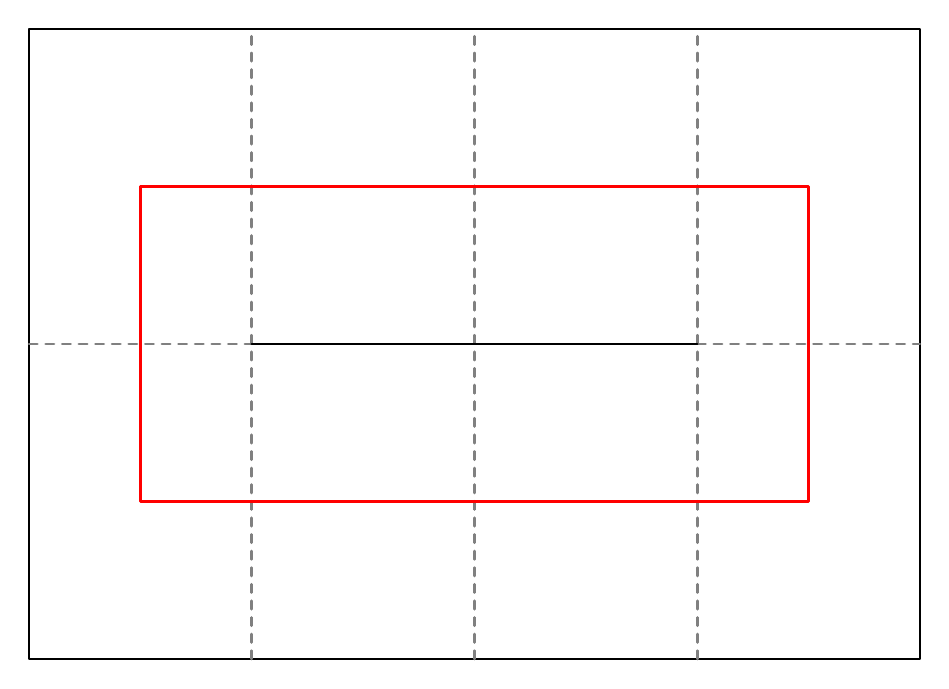
\begin{tikzpicture}[x=1.41421356cm,y=1cm,line width=1pt,line cap=round,line join=round]
\draw (0,0) rectangle (8,8);
\draw[dashed,gray]
(2,0) -- (2,8)
(4,0) -- (4,8)
(6,0) -- (6,8)
(0,4) -- (2,4) (6,4) -- (8,4);
\draw (2,4) -- (6,4);
\draw[red] (1,2) -- (1,6) -- (7,6) -- (7,2) -- cycle; 
\end{tikzpicture}
\hspace{5mm}
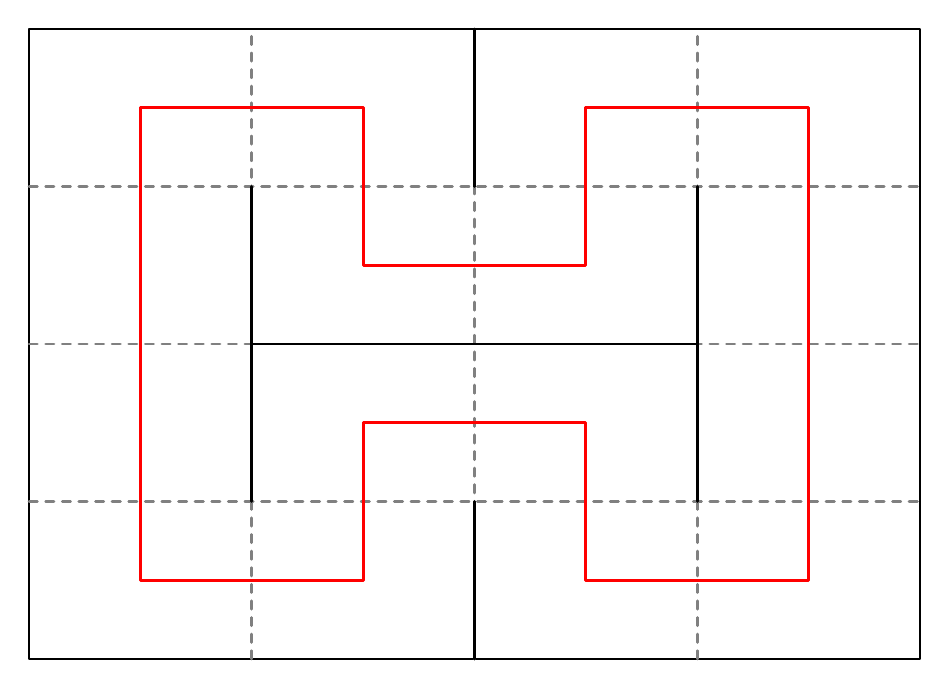
\begin{tikzpicture}[x=1.41421356cm,y=1cm,line width=1pt,line cap=round,line join=round]
\draw (0,0) rectangle (8,8);
\draw[dashed,gray]
(2,0) -- (2,8)
(4,0) -- (4,8)
(6,0) -- (6,8)
(0,2) -- (8,2)
(0,4) -- (8,4)
(0,6) -- (8,6);
\draw (2,4) -- (6,4) (2,2) -- (2,6) (4,0) -- (4,2) (4,6) -- (4,8) (6,2) -- (6,6);
\draw[red] (1,1) -- (1,7) -- (3,7) -- (3,5) -- (5,5) -- (5,7) -- (7,7) -- (7,1) -- (5,1) -- (5,3) -- (3,3) -- (3,1) -- cycle; 
\end{tikzpicture}

\vspace{5mm}

Choices:

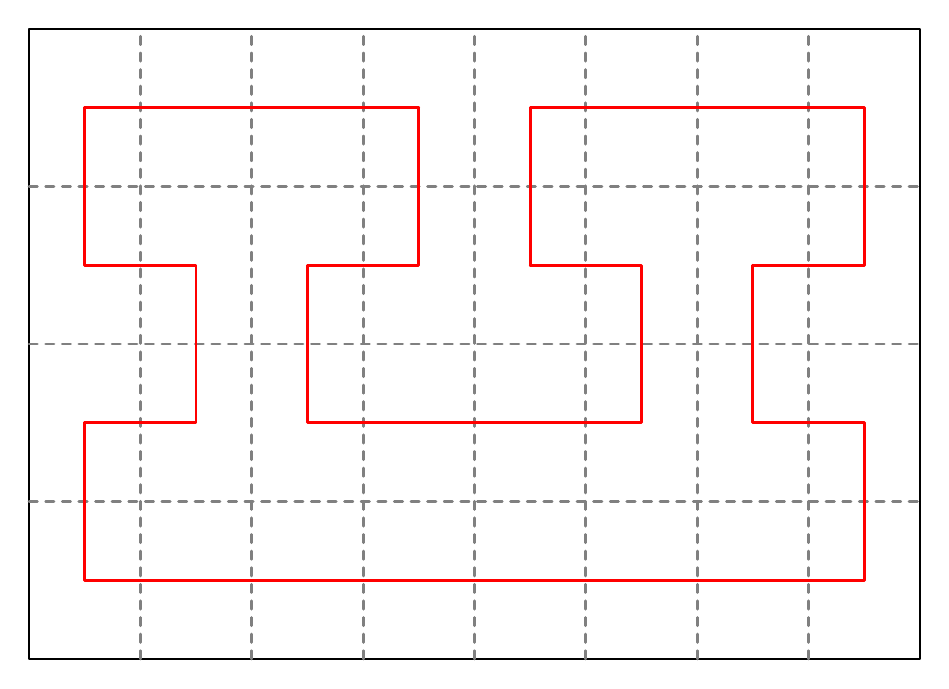
\begin{tikzpicture}[x=1.41421356cm,y=1cm,line width=1pt,line cap=round,line join=round]
\draw (0,0) rectangle (8,8);
\draw[dashed,gray]
(1,0) -- (1,8)
(2,0) -- (2,8)
(3,0) -- (3,8)
(4,0) -- (4,8)
(5,0) -- (5,8)
(6,0) -- (6,8)
(7,0) -- (7,8)
(0,2) -- (8,2)
(0,4) -- (8,4)
(0,6) -- (8,6);
%\draw (2,4) -- (6,4);
\draw[red]
    (5.5,1) -- (0.5,1) -- (0.5,3) -- (1.5,3) --
    (1.5,5) -- (0.5,5) -- (0.5,7) -- (3.5,7)
    (4.5,3) -- (2.5,3) -- (2.5,5) -- (3.5,5) -- (3.5,7)
    (5.5,1) -- (7.5,1) -- (7.5,3) -- (6.5,3) -- (6.5,5)
    (6.5,5) -- (7.5,5) -- (7.5,7) -- (4.5,7) -- (4.5,5)
    (4.5,5) -- (5.5,5) -- (5.5,3) -- (4.5,3);
\end{tikzpicture}
\hspace{5mm}
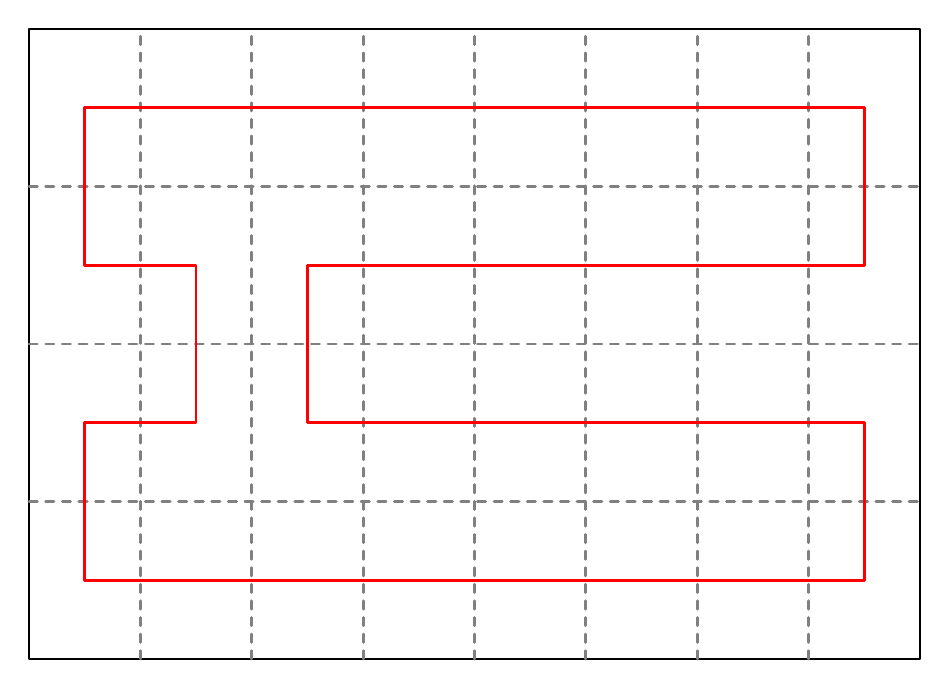
\begin{tikzpicture}[x=1.41421356cm,y=1cm,line width=1pt,line cap=round,line join=round]
\draw (0,0) rectangle (8,8);
\draw[dashed,gray]
(1,0) -- (1,8)
(2,0) -- (2,8)
(3,0) -- (3,8)
(4,0) -- (4,8)
(5,0) -- (5,8)
(6,0) -- (6,8)
(7,0) -- (7,8)
(0,2) -- (8,2)
(0,4) -- (8,4)
(0,6) -- (8,6);
%\draw (2,4) -- (6,4);
\draw[red]
    (3.5,1) -- (0.5,1) -- (0.5,3) -- (1.5,3) --
    (1.5,5) -- (0.5,5) -- (0.5,7) -- (5.5,7)
    (3.5,3) -- (2.5,3) -- (2.5,5) -- (3.5,5) -- (5.5,5)
    (3.5,1) -- (7.5,1) -- (7.5,3) -- (3.5,3)
    (5.5,5) -- (7.5,5) -- (7.5,7) -- (5.5,7);
\end{tikzpicture}

\vspace{5mm}

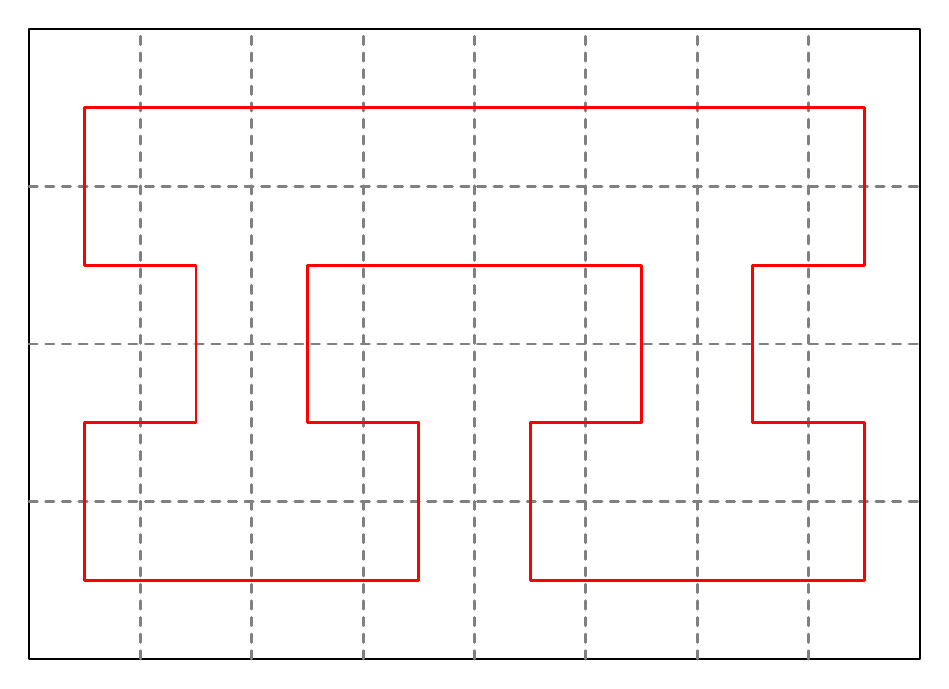
\begin{tikzpicture}[x=1.41421356cm,y=1cm,line width=1pt,line cap=round,line join=round]
\draw (0,0) rectangle (8,8);
\draw[dashed,gray]
(1,0) -- (1,8)
(2,0) -- (2,8)
(3,0) -- (3,8)
(4,0) -- (4,8)
(5,0) -- (5,8)
(6,0) -- (6,8)
(7,0) -- (7,8)
(0,2) -- (8,2)
(0,4) -- (8,4)
(0,6) -- (8,6);
%\draw (2,4) -- (6,4);
\draw[red]
    (3.5,3) -- (3.5,1) -- (0.5,1) -- (0.5,3) -- (1.5,3) --
    (1.5,5) -- (0.5,5) -- (0.5,7) -- (5.5,7)
    (3.5,3) -- (2.5,3) -- (2.5,5) -- (3.5,5) -- (5.5,5) -- (5.5,3)
    (5.5,1) -- (7.5,1) -- (7.5,3) -- (6.5,3)
    (6.5,3) -- (6.5,5) -- (7.5,5) -- (7.5,7) -- (5.5,7)
    (5.5,3) -- (4.5,3) -- (4.5,1) -- (5.5,1);
\end{tikzpicture}
\hspace{5mm}
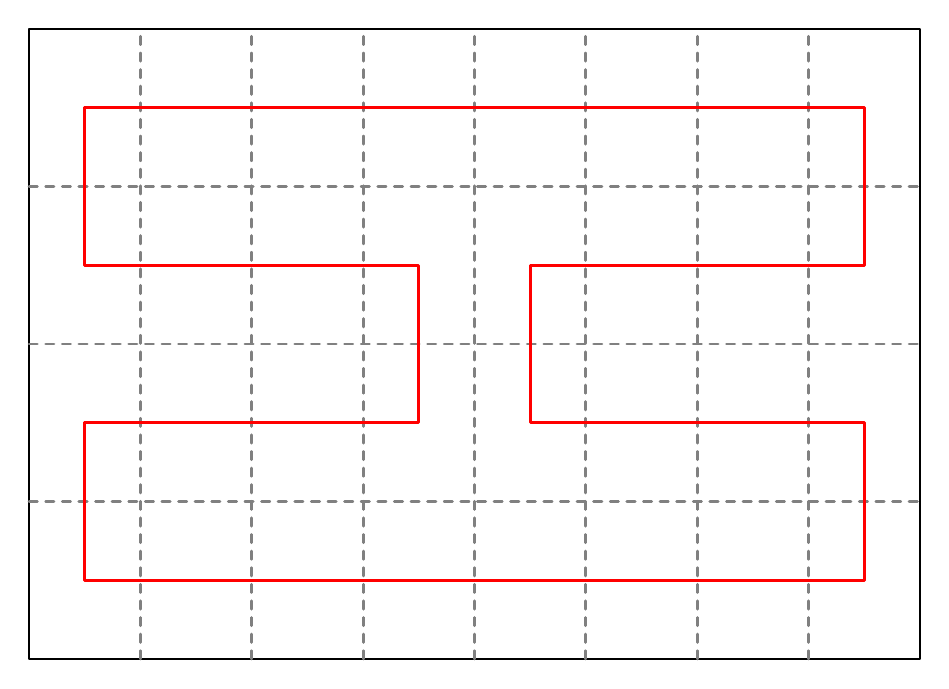
\begin{tikzpicture}[x=1.41421356cm,y=1cm,line width=1pt,line cap=round,line join=round]
\draw (0,0) rectangle (8,8);
\draw[dashed,gray]
(1,0) -- (1,8)
(2,0) -- (2,8)
(3,0) -- (3,8)
(4,0) -- (4,8)
(5,0) -- (5,8)
(6,0) -- (6,8)
(7,0) -- (7,8)
(0,2) -- (8,2)
(0,4) -- (8,4)
(0,6) -- (8,6);
%\draw (2,4) -- (6,4);
\draw[red]
    (5.5,1) -- (0.5,1) -- (0.5,3) -- (3.5,3) -- 
    (3.5,5) -- (0.5,5) -- (0.5,7) -- (5.5,7)
    (5.5,1) -- (7.5,1) -- (7.5,3) -- (6.5,3)
    (6.5,3) -- (4.5,3) -- (4.5,5) -- (7.5,5) -- (7.5,7) -- (5.5,7);
\end{tikzpicture}

\vspace{5mm}

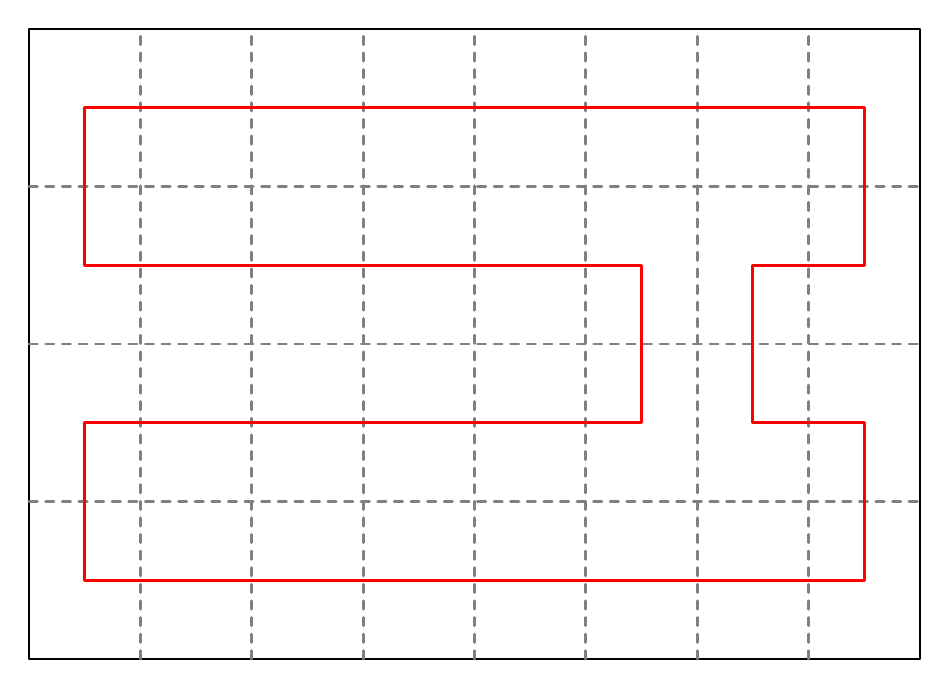
\begin{tikzpicture}[x=1.41421356cm,y=1cm,line width=1pt,line cap=round,line join=round]
\draw (0,0) rectangle (8,8);
\draw[dashed,gray]
(1,0) -- (1,8)
(2,0) -- (2,8)
(3,0) -- (3,8)
(4,0) -- (4,8)
(5,0) -- (5,8)
(6,0) -- (6,8)
(7,0) -- (7,8)
(0,2) -- (8,2)
(0,4) -- (8,4)
(0,6) -- (8,6);
%\draw (2,4) -- (6,4);
\draw[red]
    (5.5,1) -- (0.5,1) -- (0.5,3) -- (5.5,3) --
    (5.5,5) -- (0.5,5) -- (0.5,7) -- (5.5,7)
    (5.5,1) -- (7.5,1) -- (7.5,3) -- (6.5,3)
    (6.5,3) -- (6.5,5) -- (7.5,5) -- (7.5,7) -- (5.5,7);
\end{tikzpicture}

Should be invalid:
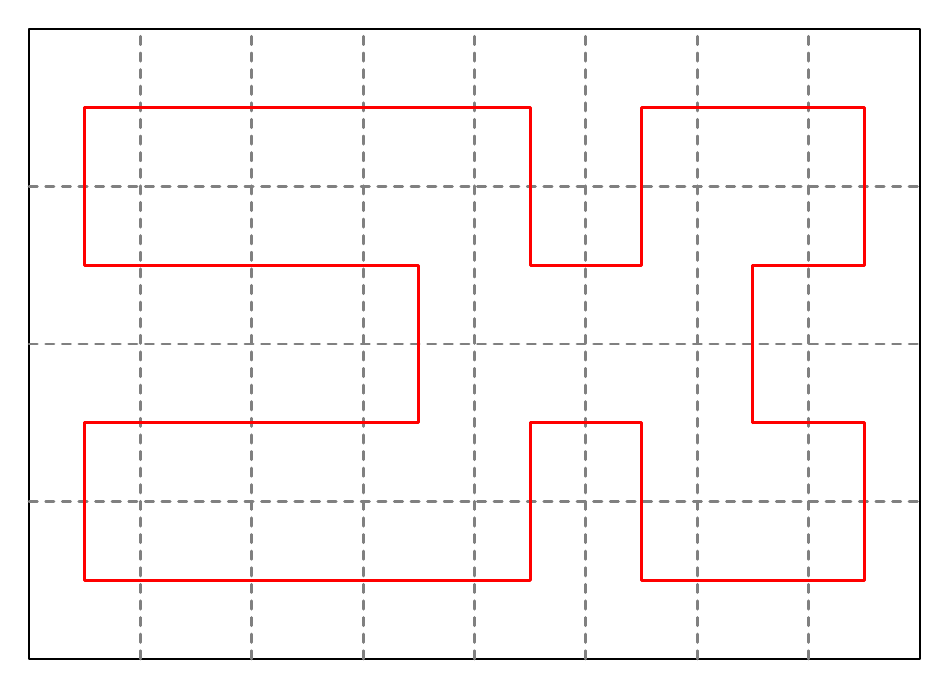
\begin{tikzpicture}[x=1.41421356cm,y=1cm,line width=1pt,line cap=round,line join=round]
\draw (0,0) rectangle (8,8);
\draw[dashed,gray]
(1,0) -- (1,8)
(2,0) -- (2,8)
(3,0) -- (3,8)
(4,0) -- (4,8)
(5,0) -- (5,8)
(6,0) -- (6,8)
(7,0) -- (7,8)
(0,2) -- (8,2)
(0,4) -- (8,4)
(0,6) -- (8,6);
%\draw (2,4) -- (6,4);
\draw[red]
    (4.5,1) -- (0.5,1) -- (0.5,3) -- (3.5,3) -- 
    (3.5,5) -- (0.5,5) -- (0.5,7) -- (4.5,7) -- (4.5,5) -- (5.5,5) -- (5.5,7)
    (4.5,1) -- (4.5,3) -- (5.5,3) -- (5.5,1) -- (7.5,1) -- (7.5,3) -- (6.5,3)
    (6.5,3) -- (6.5,5) -- (7.5,5) -- (7.5,7) -- (5.5,7);
\end{tikzpicture}

\newpage

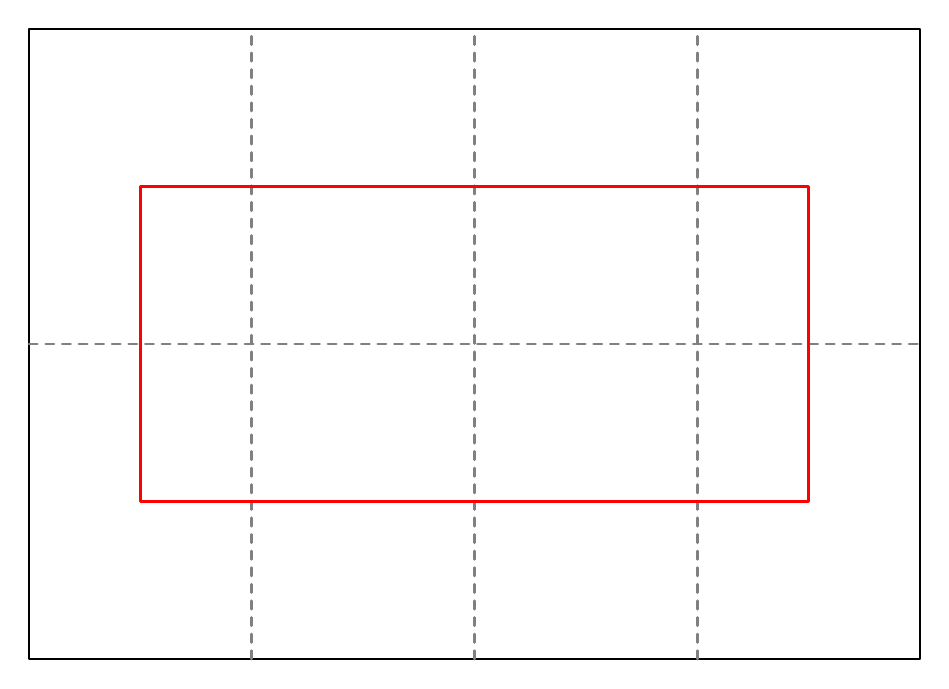
\begin{tikzpicture}[x=2.8284271247461903cm,y=4.0cm,line width=1pt,line cap=round,line join=round]
\draw (0,0) rectangle (4,2);
\draw[dashed,gray] (1,0) -- (1,2) (2,0) -- (2,2) (3,0) -- (3,2) (0,1) -- (4,1);
\draw[red] (0.5,0.5) -- (1.5,0.5) -- (2.5,0.5) -- (3.5,0.5) -- (3.5,1.5) -- (2.5,1.5) -- (1.5,1.5) -- (0.5,1.5) -- (0.5,0.5) -- cycle;\end{tikzpicture}
\hspace{5mm}
\newpage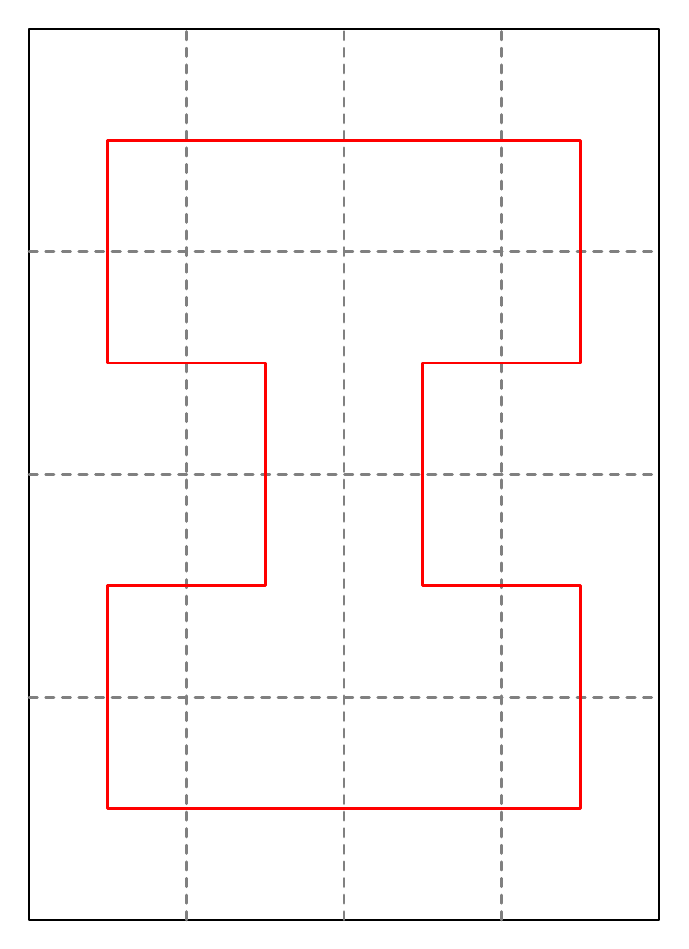
\begin{tikzpicture}[x=2.0cm,y=2.8284271247461903cm,line width=1pt,line cap=round,line join=round]
\draw (0,0) rectangle (4,4);
\draw[dashed,gray] (1,0) -- (1,4) (2,0) -- (2,4) (3,0) -- (3,4) (0,1) -- (4,1) (0,2) -- (4,2) (0,3) -- (4,3);
\draw[red] (0.5,0.5) -- (1.5,0.5) -- (2.5,0.5) -- (3.5,0.5) -- (3.5,1.5) -- (2.5,1.5) -- (2.5,2.5) -- (3.5,2.5) -- (3.5,3.5) -- (2.5,3.5) -- (1.5,3.5) -- (0.5,3.5) -- (0.5,2.5) -- (1.5,2.5) -- (1.5,1.5) -- (0.5,1.5) -- (0.5,0.5) -- cycle;\end{tikzpicture}
\hspace{5mm}
\newpage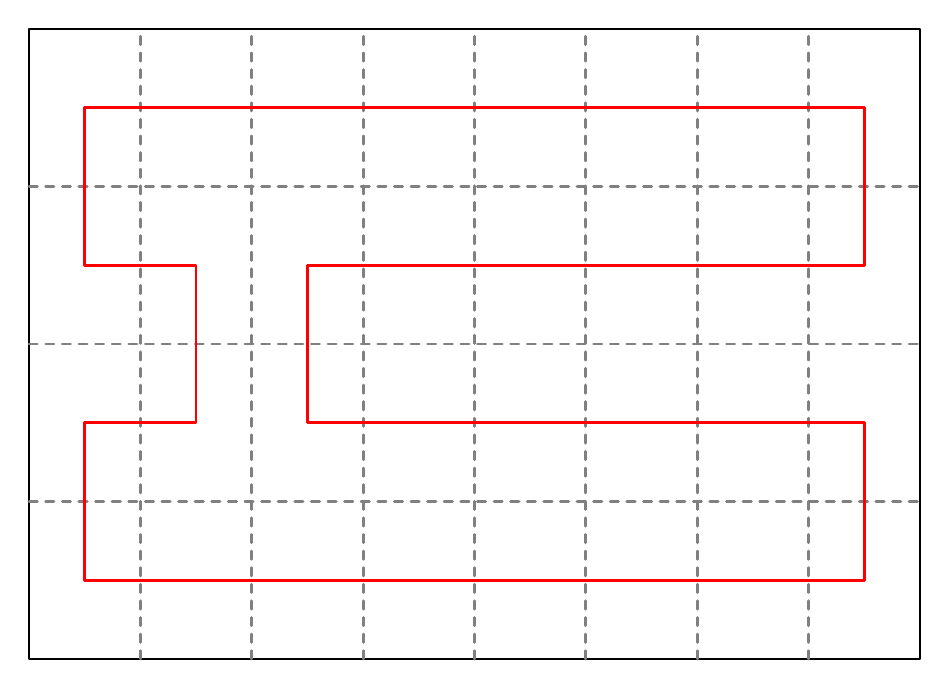
\begin{tikzpicture}[x=1.4142135623730951cm,y=2.0cm,line width=1pt,line cap=round,line join=round]
\draw (0,0) rectangle (8,4);
\draw[dashed,gray] (1,0) -- (1,4) (2,0) -- (2,4) (3,0) -- (3,4) (4,0) -- (4,4) (5,0) -- (5,4) (6,0) -- (6,4) (7,0) -- (7,4) (0,1) -- (8,1) (0,2) -- (8,2) (0,3) -- (8,3);
\draw[red] (0.5,0.5) -- (1.5,0.5) -- (2.5,0.5) -- (3.5,0.5) -- (4.5,0.5) -- (5.5,0.5) -- (6.5,0.5) -- (7.5,0.5) -- (7.5,1.5) -- (6.5,1.5) -- (5.5,1.5) -- (4.5,1.5) -- (3.5,1.5) -- (2.5,1.5) -- (2.5,2.5) -- (3.5,2.5) -- (4.5,2.5) -- (5.5,2.5) -- (6.5,2.5) -- (7.5,2.5) -- (7.5,3.5) -- (6.5,3.5) -- (5.5,3.5) -- (4.5,3.5) -- (3.5,3.5) -- (2.5,3.5) -- (1.5,3.5) -- (0.5,3.5) -- (0.5,2.5) -- (1.5,2.5) -- (1.5,1.5) -- (0.5,1.5) -- (0.5,0.5) -- cycle;\end{tikzpicture}
\hspace{5mm}
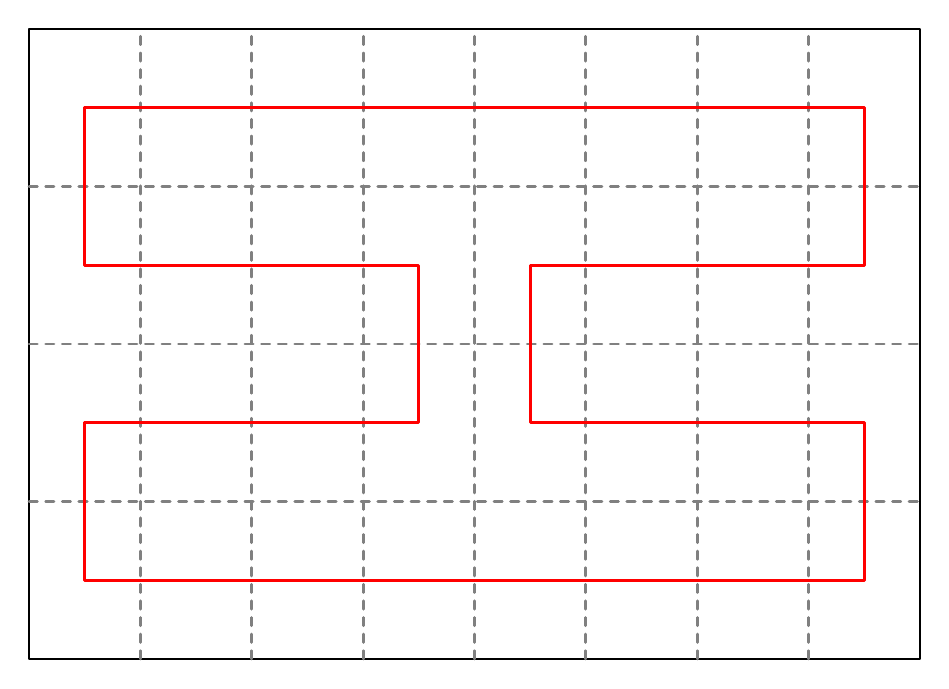
\begin{tikzpicture}[x=1.4142135623730951cm,y=2.0cm,line width=1pt,line cap=round,line join=round]
\draw (0,0) rectangle (8,4);
\draw[dashed,gray] (1,0) -- (1,4) (2,0) -- (2,4) (3,0) -- (3,4) (4,0) -- (4,4) (5,0) -- (5,4) (6,0) -- (6,4) (7,0) -- (7,4) (0,1) -- (8,1) (0,2) -- (8,2) (0,3) -- (8,3);
\draw[red] (0.5,0.5) -- (1.5,0.5) -- (2.5,0.5) -- (3.5,0.5) -- (4.5,0.5) -- (5.5,0.5) -- (6.5,0.5) -- (7.5,0.5) -- (7.5,1.5) -- (6.5,1.5) -- (5.5,1.5) -- (4.5,1.5) -- (4.5,2.5) -- (5.5,2.5) -- (6.5,2.5) -- (7.5,2.5) -- (7.5,3.5) -- (6.5,3.5) -- (5.5,3.5) -- (4.5,3.5) -- (3.5,3.5) -- (2.5,3.5) -- (1.5,3.5) -- (0.5,3.5) -- (0.5,2.5) -- (1.5,2.5) -- (2.5,2.5) -- (3.5,2.5) -- (3.5,1.5) -- (2.5,1.5) -- (1.5,1.5) -- (0.5,1.5) -- (0.5,0.5) -- cycle;\end{tikzpicture}

\vspace{5mm}

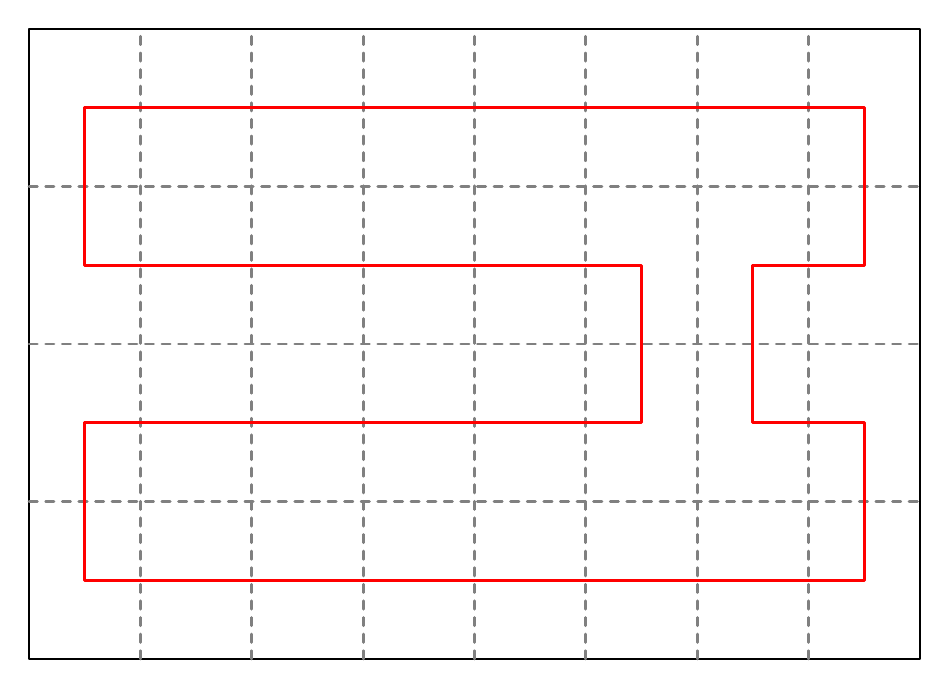
\begin{tikzpicture}[x=1.4142135623730951cm,y=2.0cm,line width=1pt,line cap=round,line join=round]
\draw (0,0) rectangle (8,4);
\draw[dashed,gray] (1,0) -- (1,4) (2,0) -- (2,4) (3,0) -- (3,4) (4,0) -- (4,4) (5,0) -- (5,4) (6,0) -- (6,4) (7,0) -- (7,4) (0,1) -- (8,1) (0,2) -- (8,2) (0,3) -- (8,3);
\draw[red] (0.5,0.5) -- (1.5,0.5) -- (2.5,0.5) -- (3.5,0.5) -- (4.5,0.5) -- (5.5,0.5) -- (6.5,0.5) -- (7.5,0.5) -- (7.5,1.5) -- (6.5,1.5) -- (6.5,2.5) -- (7.5,2.5) -- (7.5,3.5) -- (6.5,3.5) -- (5.5,3.5) -- (4.5,3.5) -- (3.5,3.5) -- (2.5,3.5) -- (1.5,3.5) -- (0.5,3.5) -- (0.5,2.5) -- (1.5,2.5) -- (2.5,2.5) -- (3.5,2.5) -- (4.5,2.5) -- (5.5,2.5) -- (5.5,1.5) -- (4.5,1.5) -- (3.5,1.5) -- (2.5,1.5) -- (1.5,1.5) -- (0.5,1.5) -- (0.5,0.5) -- cycle;\end{tikzpicture}
\hspace{5mm}
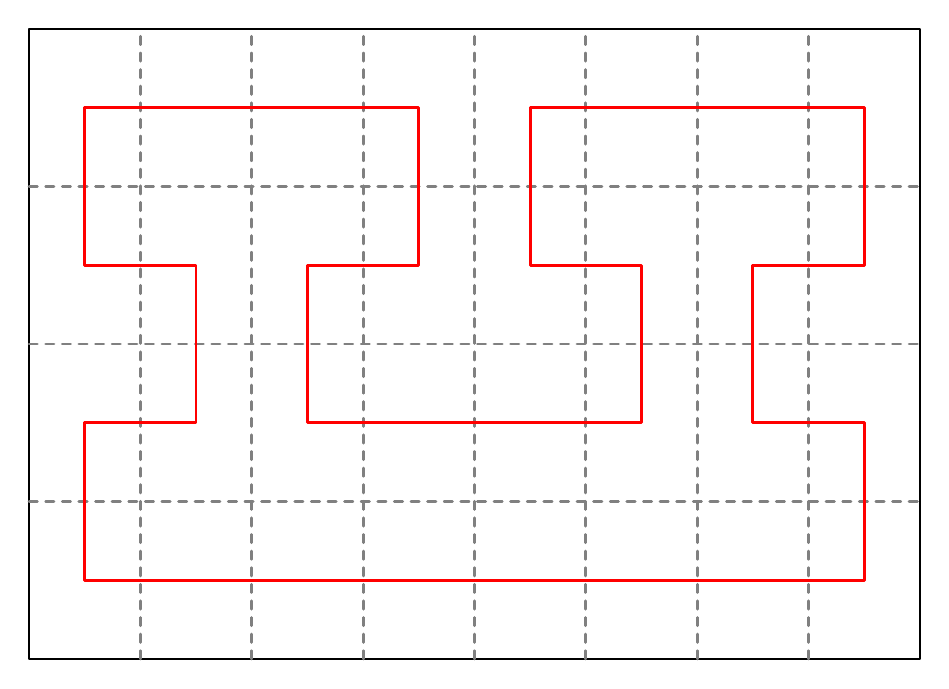
\begin{tikzpicture}[x=1.4142135623730951cm,y=2.0cm,line width=1pt,line cap=round,line join=round]
\draw (0,0) rectangle (8,4);
\draw[dashed,gray] (1,0) -- (1,4) (2,0) -- (2,4) (3,0) -- (3,4) (4,0) -- (4,4) (5,0) -- (5,4) (6,0) -- (6,4) (7,0) -- (7,4) (0,1) -- (8,1) (0,2) -- (8,2) (0,3) -- (8,3);
\draw[red] (0.5,0.5) -- (1.5,0.5) -- (2.5,0.5) -- (3.5,0.5) -- (4.5,0.5) -- (5.5,0.5) -- (6.5,0.5) -- (7.5,0.5) -- (7.5,1.5) -- (6.5,1.5) -- (6.5,2.5) -- (7.5,2.5) -- (7.5,3.5) -- (6.5,3.5) -- (5.5,3.5) -- (4.5,3.5) -- (4.5,2.5) -- (5.5,2.5) -- (5.5,1.5) -- (4.5,1.5) -- (3.5,1.5) -- (2.5,1.5) -- (2.5,2.5) -- (3.5,2.5) -- (3.5,3.5) -- (2.5,3.5) -- (1.5,3.5) -- (0.5,3.5) -- (0.5,2.5) -- (1.5,2.5) -- (1.5,1.5) -- (0.5,1.5) -- (0.5,0.5) -- cycle;\end{tikzpicture}

\vspace{5mm}

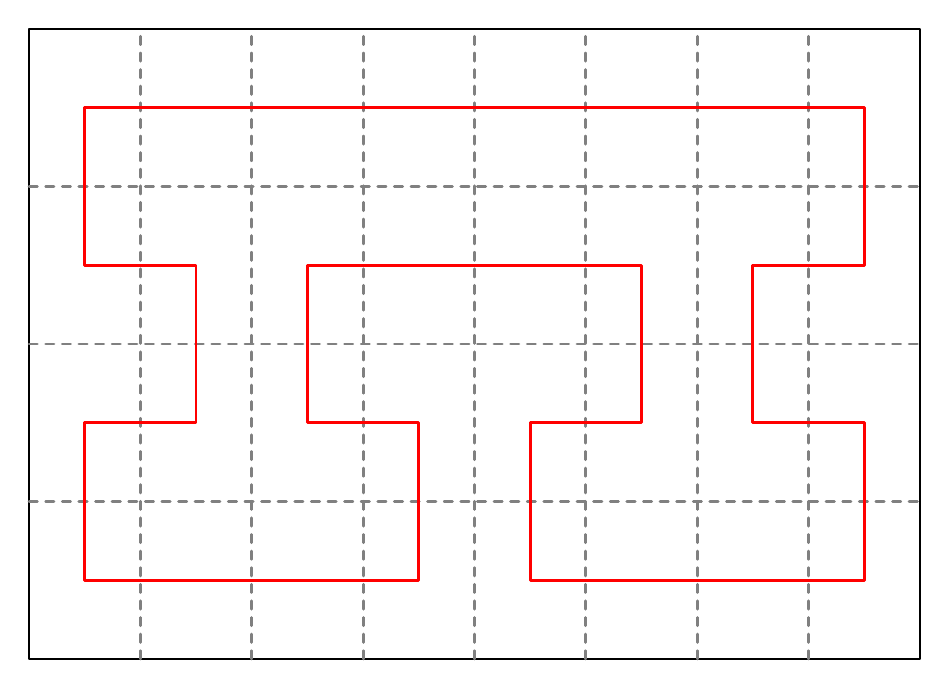
\begin{tikzpicture}[x=1.4142135623730951cm,y=2.0cm,line width=1pt,line cap=round,line join=round]
\draw (0,0) rectangle (8,4);
\draw[dashed,gray] (1,0) -- (1,4) (2,0) -- (2,4) (3,0) -- (3,4) (4,0) -- (4,4) (5,0) -- (5,4) (6,0) -- (6,4) (7,0) -- (7,4) (0,1) -- (8,1) (0,2) -- (8,2) (0,3) -- (8,3);
\draw[red] (0.5,0.5) -- (1.5,0.5) -- (2.5,0.5) -- (3.5,0.5) -- (3.5,1.5) -- (2.5,1.5) -- (2.5,2.5) -- (3.5,2.5) -- (4.5,2.5) -- (5.5,2.5) -- (5.5,1.5) -- (4.5,1.5) -- (4.5,0.5) -- (5.5,0.5) -- (6.5,0.5) -- (7.5,0.5) -- (7.5,1.5) -- (6.5,1.5) -- (6.5,2.5) -- (7.5,2.5) -- (7.5,3.5) -- (6.5,3.5) -- (5.5,3.5) -- (4.5,3.5) -- (3.5,3.5) -- (2.5,3.5) -- (1.5,3.5) -- (0.5,3.5) -- (0.5,2.5) -- (1.5,2.5) -- (1.5,1.5) -- (0.5,1.5) -- (0.5,0.5) -- cycle;\end{tikzpicture}
\hspace{5mm}
\newpage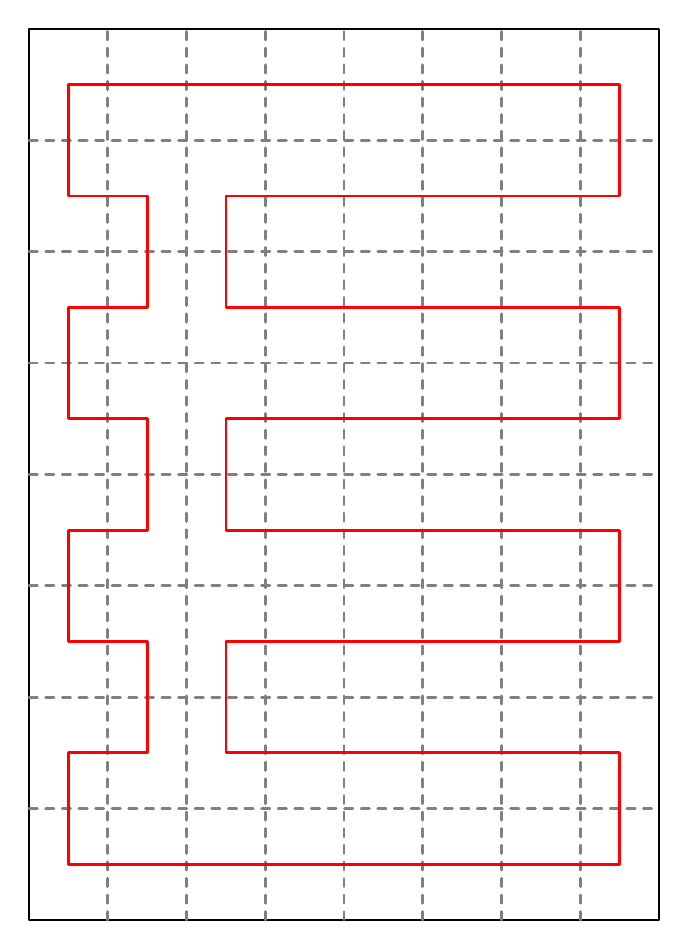
\begin{tikzpicture}[x=1.0cm,y=1.4142135623730951cm,line width=1pt,line cap=round,line join=round]
\draw (0,0) rectangle (8,8);
\draw[dashed,gray] (1,0) -- (1,8) (2,0) -- (2,8) (3,0) -- (3,8) (4,0) -- (4,8) (5,0) -- (5,8) (6,0) -- (6,8) (7,0) -- (7,8) (0,1) -- (8,1) (0,2) -- (8,2) (0,3) -- (8,3) (0,4) -- (8,4) (0,5) -- (8,5) (0,6) -- (8,6) (0,7) -- (8,7);
\draw[red] (0.5,0.5) -- (1.5,0.5) -- (2.5,0.5) -- (3.5,0.5) -- (4.5,0.5) -- (5.5,0.5) -- (6.5,0.5) -- (7.5,0.5) -- (7.5,1.5) -- (6.5,1.5) -- (5.5,1.5) -- (4.5,1.5) -- (3.5,1.5) -- (2.5,1.5) -- (2.5,2.5) -- (3.5,2.5) -- (4.5,2.5) -- (5.5,2.5) -- (6.5,2.5) -- (7.5,2.5) -- (7.5,3.5) -- (6.5,3.5) -- (5.5,3.5) -- (4.5,3.5) -- (3.5,3.5) -- (2.5,3.5) -- (2.5,4.5) -- (3.5,4.5) -- (4.5,4.5) -- (5.5,4.5) -- (6.5,4.5) -- (7.5,4.5) -- (7.5,5.5) -- (6.5,5.5) -- (5.5,5.5) -- (4.5,5.5) -- (3.5,5.5) -- (2.5,5.5) -- (2.5,6.5) -- (3.5,6.5) -- (4.5,6.5) -- (5.5,6.5) -- (6.5,6.5) -- (7.5,6.5) -- (7.5,7.5) -- (6.5,7.5) -- (5.5,7.5) -- (4.5,7.5) -- (3.5,7.5) -- (2.5,7.5) -- (1.5,7.5) -- (0.5,7.5) -- (0.5,6.5) -- (1.5,6.5) -- (1.5,5.5) -- (0.5,5.5) -- (0.5,4.5) -- (1.5,4.5) -- (1.5,3.5) -- (0.5,3.5) -- (0.5,2.5) -- (1.5,2.5) -- (1.5,1.5) -- (0.5,1.5) -- (0.5,0.5) -- cycle;\end{tikzpicture}
\hspace{5mm}
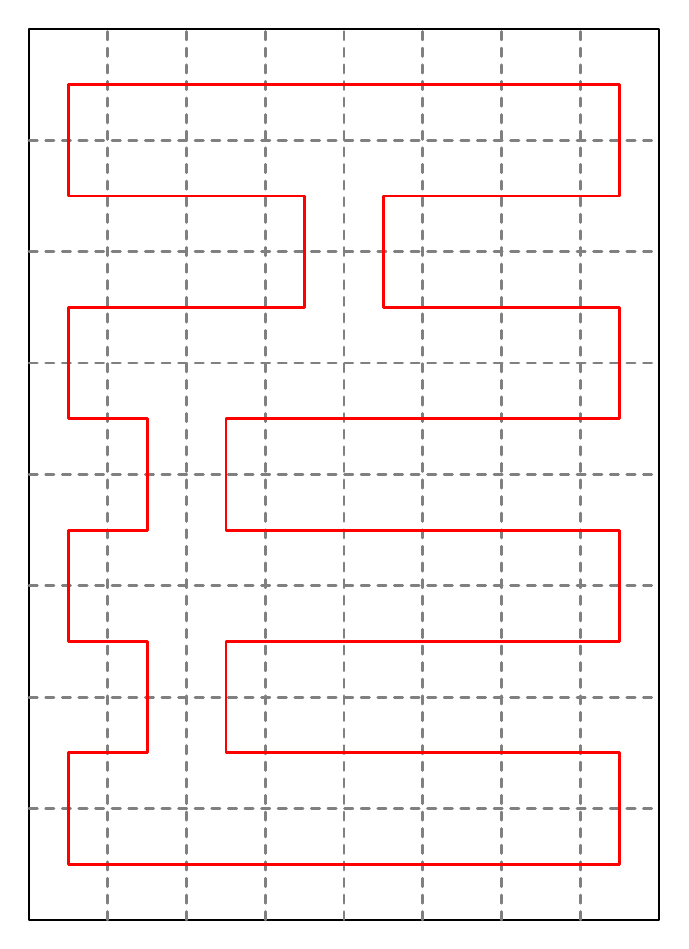
\begin{tikzpicture}[x=1.0cm,y=1.4142135623730951cm,line width=1pt,line cap=round,line join=round]
\draw (0,0) rectangle (8,8);
\draw[dashed,gray] (1,0) -- (1,8) (2,0) -- (2,8) (3,0) -- (3,8) (4,0) -- (4,8) (5,0) -- (5,8) (6,0) -- (6,8) (7,0) -- (7,8) (0,1) -- (8,1) (0,2) -- (8,2) (0,3) -- (8,3) (0,4) -- (8,4) (0,5) -- (8,5) (0,6) -- (8,6) (0,7) -- (8,7);
\draw[red] (0.5,0.5) -- (1.5,0.5) -- (2.5,0.5) -- (3.5,0.5) -- (4.5,0.5) -- (5.5,0.5) -- (6.5,0.5) -- (7.5,0.5) -- (7.5,1.5) -- (6.5,1.5) -- (5.5,1.5) -- (4.5,1.5) -- (3.5,1.5) -- (2.5,1.5) -- (2.5,2.5) -- (3.5,2.5) -- (4.5,2.5) -- (5.5,2.5) -- (6.5,2.5) -- (7.5,2.5) -- (7.5,3.5) -- (6.5,3.5) -- (5.5,3.5) -- (4.5,3.5) -- (3.5,3.5) -- (2.5,3.5) -- (2.5,4.5) -- (3.5,4.5) -- (4.5,4.5) -- (5.5,4.5) -- (6.5,4.5) -- (7.5,4.5) -- (7.5,5.5) -- (6.5,5.5) -- (5.5,5.5) -- (4.5,5.5) -- (4.5,6.5) -- (5.5,6.5) -- (6.5,6.5) -- (7.5,6.5) -- (7.5,7.5) -- (6.5,7.5) -- (5.5,7.5) -- (4.5,7.5) -- (3.5,7.5) -- (2.5,7.5) -- (1.5,7.5) -- (0.5,7.5) -- (0.5,6.5) -- (1.5,6.5) -- (2.5,6.5) -- (3.5,6.5) -- (3.5,5.5) -- (2.5,5.5) -- (1.5,5.5) -- (0.5,5.5) -- (0.5,4.5) -- (1.5,4.5) -- (1.5,3.5) -- (0.5,3.5) -- (0.5,2.5) -- (1.5,2.5) -- (1.5,1.5) -- (0.5,1.5) -- (0.5,0.5) -- cycle;\end{tikzpicture}

\vspace{5mm}

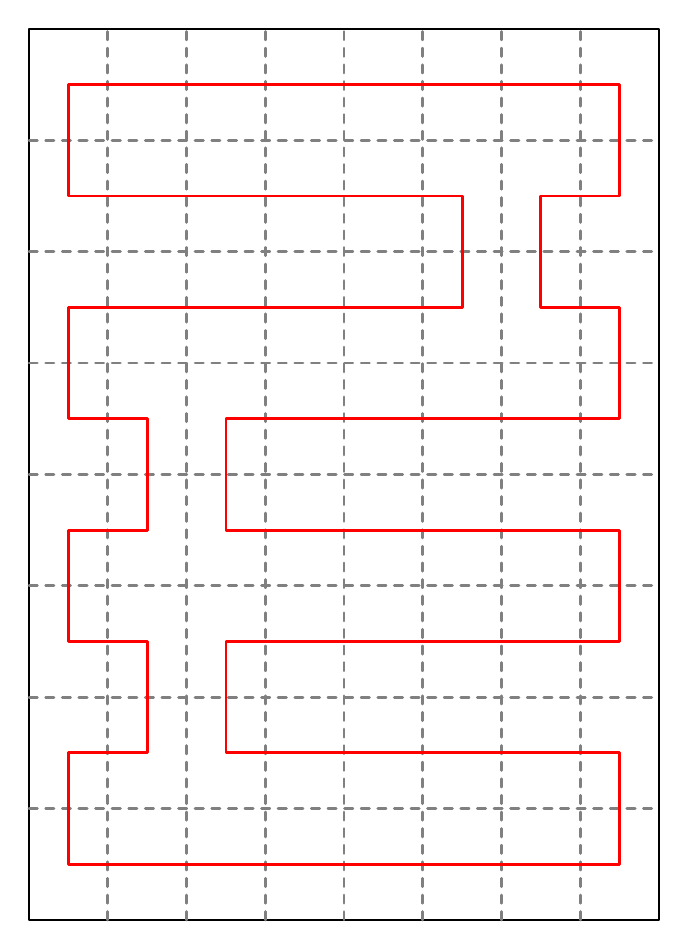
\begin{tikzpicture}[x=1.0cm,y=1.4142135623730951cm,line width=1pt,line cap=round,line join=round]
\draw (0,0) rectangle (8,8);
\draw[dashed,gray] (1,0) -- (1,8) (2,0) -- (2,8) (3,0) -- (3,8) (4,0) -- (4,8) (5,0) -- (5,8) (6,0) -- (6,8) (7,0) -- (7,8) (0,1) -- (8,1) (0,2) -- (8,2) (0,3) -- (8,3) (0,4) -- (8,4) (0,5) -- (8,5) (0,6) -- (8,6) (0,7) -- (8,7);
\draw[red] (0.5,0.5) -- (1.5,0.5) -- (2.5,0.5) -- (3.5,0.5) -- (4.5,0.5) -- (5.5,0.5) -- (6.5,0.5) -- (7.5,0.5) -- (7.5,1.5) -- (6.5,1.5) -- (5.5,1.5) -- (4.5,1.5) -- (3.5,1.5) -- (2.5,1.5) -- (2.5,2.5) -- (3.5,2.5) -- (4.5,2.5) -- (5.5,2.5) -- (6.5,2.5) -- (7.5,2.5) -- (7.5,3.5) -- (6.5,3.5) -- (5.5,3.5) -- (4.5,3.5) -- (3.5,3.5) -- (2.5,3.5) -- (2.5,4.5) -- (3.5,4.5) -- (4.5,4.5) -- (5.5,4.5) -- (6.5,4.5) -- (7.5,4.5) -- (7.5,5.5) -- (6.5,5.5) -- (6.5,6.5) -- (7.5,6.5) -- (7.5,7.5) -- (6.5,7.5) -- (5.5,7.5) -- (4.5,7.5) -- (3.5,7.5) -- (2.5,7.5) -- (1.5,7.5) -- (0.5,7.5) -- (0.5,6.5) -- (1.5,6.5) -- (2.5,6.5) -- (3.5,6.5) -- (4.5,6.5) -- (5.5,6.5) -- (5.5,5.5) -- (4.5,5.5) -- (3.5,5.5) -- (2.5,5.5) -- (1.5,5.5) -- (0.5,5.5) -- (0.5,4.5) -- (1.5,4.5) -- (1.5,3.5) -- (0.5,3.5) -- (0.5,2.5) -- (1.5,2.5) -- (1.5,1.5) -- (0.5,1.5) -- (0.5,0.5) -- cycle;\end{tikzpicture}
\hspace{5mm}
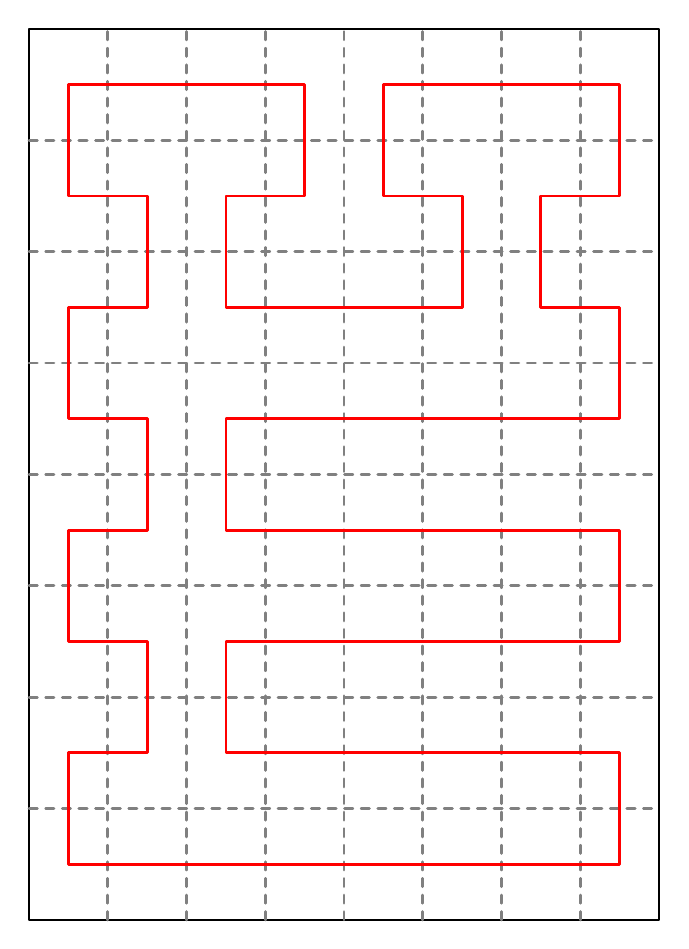
\begin{tikzpicture}[x=1.0cm,y=1.4142135623730951cm,line width=1pt,line cap=round,line join=round]
\draw (0,0) rectangle (8,8);
\draw[dashed,gray] (1,0) -- (1,8) (2,0) -- (2,8) (3,0) -- (3,8) (4,0) -- (4,8) (5,0) -- (5,8) (6,0) -- (6,8) (7,0) -- (7,8) (0,1) -- (8,1) (0,2) -- (8,2) (0,3) -- (8,3) (0,4) -- (8,4) (0,5) -- (8,5) (0,6) -- (8,6) (0,7) -- (8,7);
\draw[red] (0.5,0.5) -- (1.5,0.5) -- (2.5,0.5) -- (3.5,0.5) -- (4.5,0.5) -- (5.5,0.5) -- (6.5,0.5) -- (7.5,0.5) -- (7.5,1.5) -- (6.5,1.5) -- (5.5,1.5) -- (4.5,1.5) -- (3.5,1.5) -- (2.5,1.5) -- (2.5,2.5) -- (3.5,2.5) -- (4.5,2.5) -- (5.5,2.5) -- (6.5,2.5) -- (7.5,2.5) -- (7.5,3.5) -- (6.5,3.5) -- (5.5,3.5) -- (4.5,3.5) -- (3.5,3.5) -- (2.5,3.5) -- (2.5,4.5) -- (3.5,4.5) -- (4.5,4.5) -- (5.5,4.5) -- (6.5,4.5) -- (7.5,4.5) -- (7.5,5.5) -- (6.5,5.5) -- (6.5,6.5) -- (7.5,6.5) -- (7.5,7.5) -- (6.5,7.5) -- (5.5,7.5) -- (4.5,7.5) -- (4.5,6.5) -- (5.5,6.5) -- (5.5,5.5) -- (4.5,5.5) -- (3.5,5.5) -- (2.5,5.5) -- (2.5,6.5) -- (3.5,6.5) -- (3.5,7.5) -- (2.5,7.5) -- (1.5,7.5) -- (0.5,7.5) -- (0.5,6.5) -- (1.5,6.5) -- (1.5,5.5) -- (0.5,5.5) -- (0.5,4.5) -- (1.5,4.5) -- (1.5,3.5) -- (0.5,3.5) -- (0.5,2.5) -- (1.5,2.5) -- (1.5,1.5) -- (0.5,1.5) -- (0.5,0.5) -- cycle;\end{tikzpicture}

\vspace{5mm}

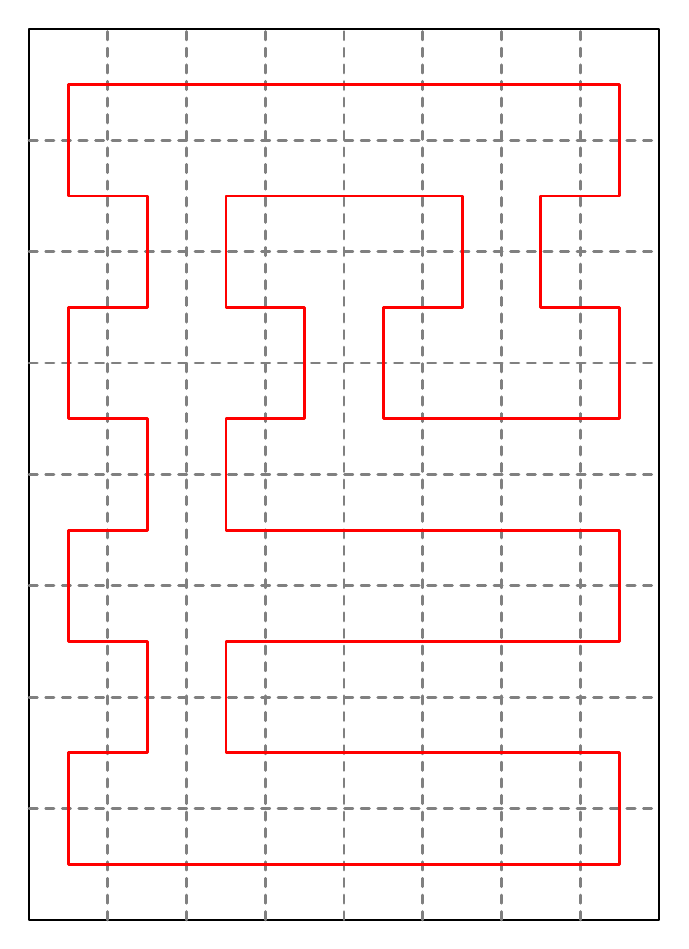
\begin{tikzpicture}[x=1.0cm,y=1.4142135623730951cm,line width=1pt,line cap=round,line join=round]
\draw (0,0) rectangle (8,8);
\draw[dashed,gray] (1,0) -- (1,8) (2,0) -- (2,8) (3,0) -- (3,8) (4,0) -- (4,8) (5,0) -- (5,8) (6,0) -- (6,8) (7,0) -- (7,8) (0,1) -- (8,1) (0,2) -- (8,2) (0,3) -- (8,3) (0,4) -- (8,4) (0,5) -- (8,5) (0,6) -- (8,6) (0,7) -- (8,7);
\draw[red] (0.5,0.5) -- (1.5,0.5) -- (2.5,0.5) -- (3.5,0.5) -- (4.5,0.5) -- (5.5,0.5) -- (6.5,0.5) -- (7.5,0.5) -- (7.5,1.5) -- (6.5,1.5) -- (5.5,1.5) -- (4.5,1.5) -- (3.5,1.5) -- (2.5,1.5) -- (2.5,2.5) -- (3.5,2.5) -- (4.5,2.5) -- (5.5,2.5) -- (6.5,2.5) -- (7.5,2.5) -- (7.5,3.5) -- (6.5,3.5) -- (5.5,3.5) -- (4.5,3.5) -- (3.5,3.5) -- (2.5,3.5) -- (2.5,4.5) -- (3.5,4.5) -- (3.5,5.5) -- (2.5,5.5) -- (2.5,6.5) -- (3.5,6.5) -- (4.5,6.5) -- (5.5,6.5) -- (5.5,5.5) -- (4.5,5.5) -- (4.5,4.5) -- (5.5,4.5) -- (6.5,4.5) -- (7.5,4.5) -- (7.5,5.5) -- (6.5,5.5) -- (6.5,6.5) -- (7.5,6.5) -- (7.5,7.5) -- (6.5,7.5) -- (5.5,7.5) -- (4.5,7.5) -- (3.5,7.5) -- (2.5,7.5) -- (1.5,7.5) -- (0.5,7.5) -- (0.5,6.5) -- (1.5,6.5) -- (1.5,5.5) -- (0.5,5.5) -- (0.5,4.5) -- (1.5,4.5) -- (1.5,3.5) -- (0.5,3.5) -- (0.5,2.5) -- (1.5,2.5) -- (1.5,1.5) -- (0.5,1.5) -- (0.5,0.5) -- cycle;\end{tikzpicture}
\hspace{5mm}
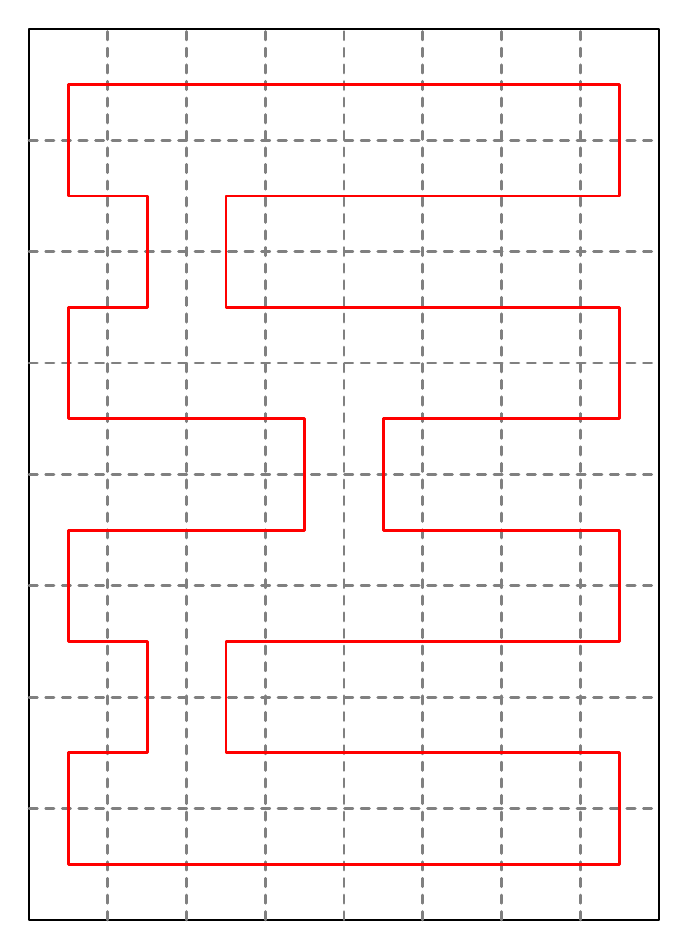
\begin{tikzpicture}[x=1.0cm,y=1.4142135623730951cm,line width=1pt,line cap=round,line join=round]
\draw (0,0) rectangle (8,8);
\draw[dashed,gray] (1,0) -- (1,8) (2,0) -- (2,8) (3,0) -- (3,8) (4,0) -- (4,8) (5,0) -- (5,8) (6,0) -- (6,8) (7,0) -- (7,8) (0,1) -- (8,1) (0,2) -- (8,2) (0,3) -- (8,3) (0,4) -- (8,4) (0,5) -- (8,5) (0,6) -- (8,6) (0,7) -- (8,7);
\draw[red] (0.5,0.5) -- (1.5,0.5) -- (2.5,0.5) -- (3.5,0.5) -- (4.5,0.5) -- (5.5,0.5) -- (6.5,0.5) -- (7.5,0.5) -- (7.5,1.5) -- (6.5,1.5) -- (5.5,1.5) -- (4.5,1.5) -- (3.5,1.5) -- (2.5,1.5) -- (2.5,2.5) -- (3.5,2.5) -- (4.5,2.5) -- (5.5,2.5) -- (6.5,2.5) -- (7.5,2.5) -- (7.5,3.5) -- (6.5,3.5) -- (5.5,3.5) -- (4.5,3.5) -- (4.5,4.5) -- (5.5,4.5) -- (6.5,4.5) -- (7.5,4.5) -- (7.5,5.5) -- (6.5,5.5) -- (5.5,5.5) -- (4.5,5.5) -- (3.5,5.5) -- (2.5,5.5) -- (2.5,6.5) -- (3.5,6.5) -- (4.5,6.5) -- (5.5,6.5) -- (6.5,6.5) -- (7.5,6.5) -- (7.5,7.5) -- (6.5,7.5) -- (5.5,7.5) -- (4.5,7.5) -- (3.5,7.5) -- (2.5,7.5) -- (1.5,7.5) -- (0.5,7.5) -- (0.5,6.5) -- (1.5,6.5) -- (1.5,5.5) -- (0.5,5.5) -- (0.5,4.5) -- (1.5,4.5) -- (2.5,4.5) -- (3.5,4.5) -- (3.5,3.5) -- (2.5,3.5) -- (1.5,3.5) -- (0.5,3.5) -- (0.5,2.5) -- (1.5,2.5) -- (1.5,1.5) -- (0.5,1.5) -- (0.5,0.5) -- cycle;\end{tikzpicture}

\vspace{5mm}

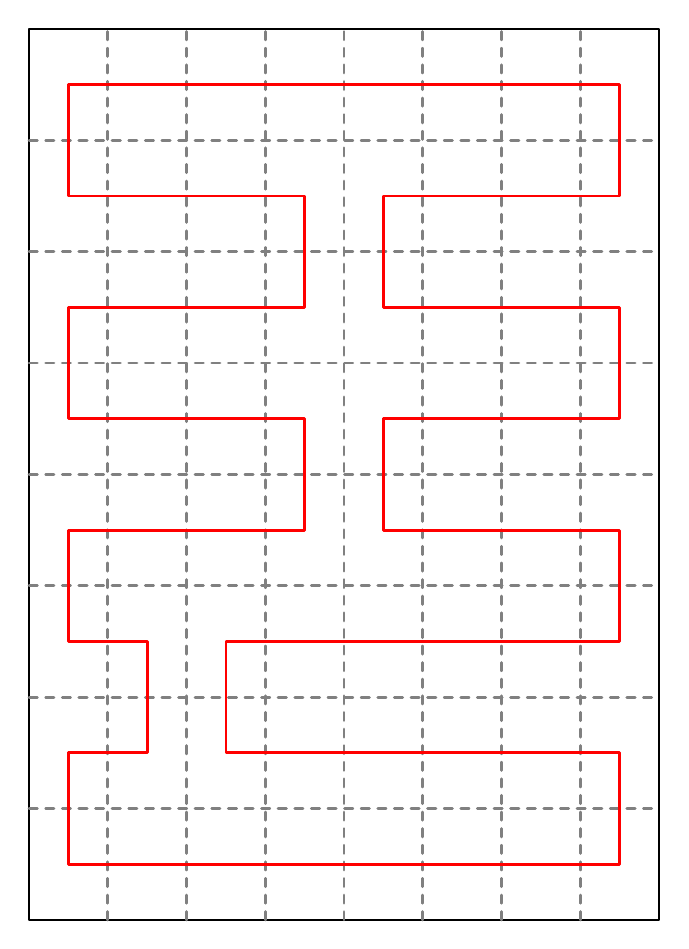
\begin{tikzpicture}[x=1.0cm,y=1.4142135623730951cm,line width=1pt,line cap=round,line join=round]
\draw (0,0) rectangle (8,8);
\draw[dashed,gray] (1,0) -- (1,8) (2,0) -- (2,8) (3,0) -- (3,8) (4,0) -- (4,8) (5,0) -- (5,8) (6,0) -- (6,8) (7,0) -- (7,8) (0,1) -- (8,1) (0,2) -- (8,2) (0,3) -- (8,3) (0,4) -- (8,4) (0,5) -- (8,5) (0,6) -- (8,6) (0,7) -- (8,7);
\draw[red] (0.5,0.5) -- (1.5,0.5) -- (2.5,0.5) -- (3.5,0.5) -- (4.5,0.5) -- (5.5,0.5) -- (6.5,0.5) -- (7.5,0.5) -- (7.5,1.5) -- (6.5,1.5) -- (5.5,1.5) -- (4.5,1.5) -- (3.5,1.5) -- (2.5,1.5) -- (2.5,2.5) -- (3.5,2.5) -- (4.5,2.5) -- (5.5,2.5) -- (6.5,2.5) -- (7.5,2.5) -- (7.5,3.5) -- (6.5,3.5) -- (5.5,3.5) -- (4.5,3.5) -- (4.5,4.5) -- (5.5,4.5) -- (6.5,4.5) -- (7.5,4.5) -- (7.5,5.5) -- (6.5,5.5) -- (5.5,5.5) -- (4.5,5.5) -- (4.5,6.5) -- (5.5,6.5) -- (6.5,6.5) -- (7.5,6.5) -- (7.5,7.5) -- (6.5,7.5) -- (5.5,7.5) -- (4.5,7.5) -- (3.5,7.5) -- (2.5,7.5) -- (1.5,7.5) -- (0.5,7.5) -- (0.5,6.5) -- (1.5,6.5) -- (2.5,6.5) -- (3.5,6.5) -- (3.5,5.5) -- (2.5,5.5) -- (1.5,5.5) -- (0.5,5.5) -- (0.5,4.5) -- (1.5,4.5) -- (2.5,4.5) -- (3.5,4.5) -- (3.5,3.5) -- (2.5,3.5) -- (1.5,3.5) -- (0.5,3.5) -- (0.5,2.5) -- (1.5,2.5) -- (1.5,1.5) -- (0.5,1.5) -- (0.5,0.5) -- cycle;\end{tikzpicture}
\hspace{5mm}
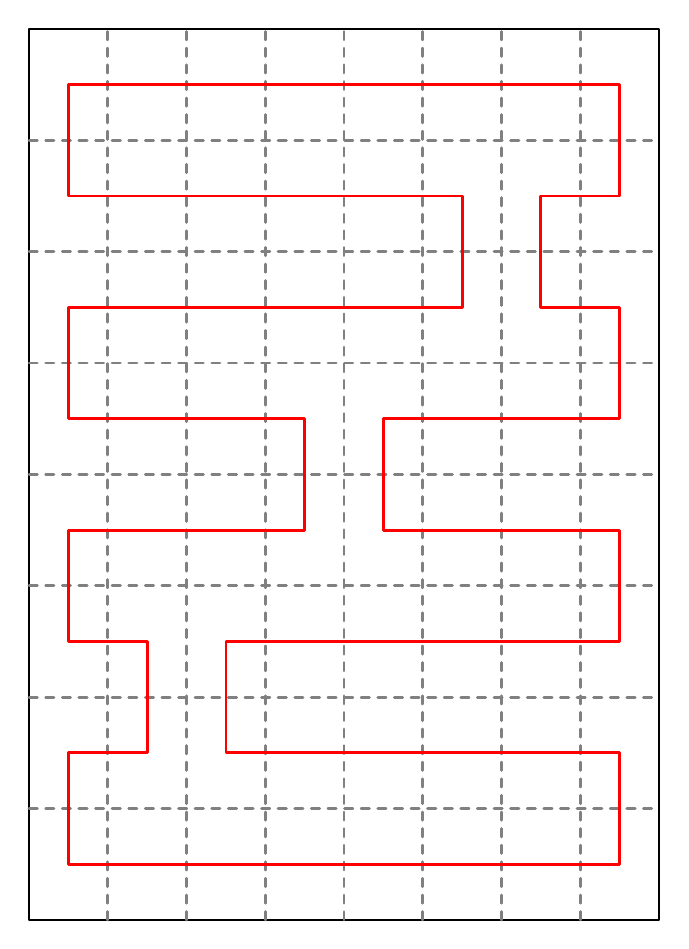
\begin{tikzpicture}[x=1.0cm,y=1.4142135623730951cm,line width=1pt,line cap=round,line join=round]
\draw (0,0) rectangle (8,8);
\draw[dashed,gray] (1,0) -- (1,8) (2,0) -- (2,8) (3,0) -- (3,8) (4,0) -- (4,8) (5,0) -- (5,8) (6,0) -- (6,8) (7,0) -- (7,8) (0,1) -- (8,1) (0,2) -- (8,2) (0,3) -- (8,3) (0,4) -- (8,4) (0,5) -- (8,5) (0,6) -- (8,6) (0,7) -- (8,7);
\draw[red] (0.5,0.5) -- (1.5,0.5) -- (2.5,0.5) -- (3.5,0.5) -- (4.5,0.5) -- (5.5,0.5) -- (6.5,0.5) -- (7.5,0.5) -- (7.5,1.5) -- (6.5,1.5) -- (5.5,1.5) -- (4.5,1.5) -- (3.5,1.5) -- (2.5,1.5) -- (2.5,2.5) -- (3.5,2.5) -- (4.5,2.5) -- (5.5,2.5) -- (6.5,2.5) -- (7.5,2.5) -- (7.5,3.5) -- (6.5,3.5) -- (5.5,3.5) -- (4.5,3.5) -- (4.5,4.5) -- (5.5,4.5) -- (6.5,4.5) -- (7.5,4.5) -- (7.5,5.5) -- (6.5,5.5) -- (6.5,6.5) -- (7.5,6.5) -- (7.5,7.5) -- (6.5,7.5) -- (5.5,7.5) -- (4.5,7.5) -- (3.5,7.5) -- (2.5,7.5) -- (1.5,7.5) -- (0.5,7.5) -- (0.5,6.5) -- (1.5,6.5) -- (2.5,6.5) -- (3.5,6.5) -- (4.5,6.5) -- (5.5,6.5) -- (5.5,5.5) -- (4.5,5.5) -- (3.5,5.5) -- (2.5,5.5) -- (1.5,5.5) -- (0.5,5.5) -- (0.5,4.5) -- (1.5,4.5) -- (2.5,4.5) -- (3.5,4.5) -- (3.5,3.5) -- (2.5,3.5) -- (1.5,3.5) -- (0.5,3.5) -- (0.5,2.5) -- (1.5,2.5) -- (1.5,1.5) -- (0.5,1.5) -- (0.5,0.5) -- cycle;\end{tikzpicture}

\vspace{5mm}

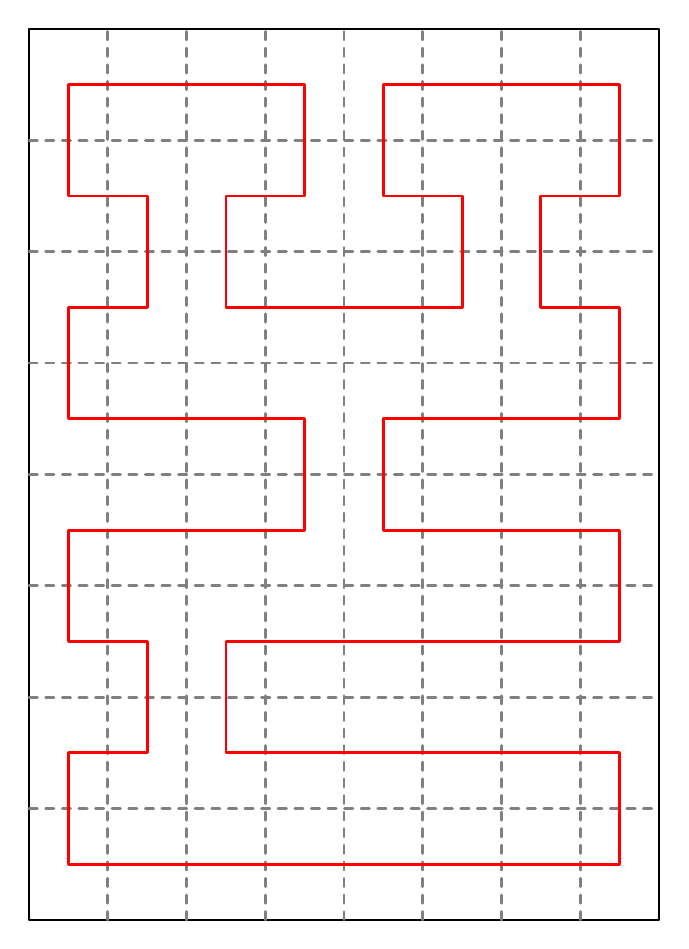
\begin{tikzpicture}[x=1.0cm,y=1.4142135623730951cm,line width=1pt,line cap=round,line join=round]
\draw (0,0) rectangle (8,8);
\draw[dashed,gray] (1,0) -- (1,8) (2,0) -- (2,8) (3,0) -- (3,8) (4,0) -- (4,8) (5,0) -- (5,8) (6,0) -- (6,8) (7,0) -- (7,8) (0,1) -- (8,1) (0,2) -- (8,2) (0,3) -- (8,3) (0,4) -- (8,4) (0,5) -- (8,5) (0,6) -- (8,6) (0,7) -- (8,7);
\draw[red] (0.5,0.5) -- (1.5,0.5) -- (2.5,0.5) -- (3.5,0.5) -- (4.5,0.5) -- (5.5,0.5) -- (6.5,0.5) -- (7.5,0.5) -- (7.5,1.5) -- (6.5,1.5) -- (5.5,1.5) -- (4.5,1.5) -- (3.5,1.5) -- (2.5,1.5) -- (2.5,2.5) -- (3.5,2.5) -- (4.5,2.5) -- (5.5,2.5) -- (6.5,2.5) -- (7.5,2.5) -- (7.5,3.5) -- (6.5,3.5) -- (5.5,3.5) -- (4.5,3.5) -- (4.5,4.5) -- (5.5,4.5) -- (6.5,4.5) -- (7.5,4.5) -- (7.5,5.5) -- (6.5,5.5) -- (6.5,6.5) -- (7.5,6.5) -- (7.5,7.5) -- (6.5,7.5) -- (5.5,7.5) -- (4.5,7.5) -- (4.5,6.5) -- (5.5,6.5) -- (5.5,5.5) -- (4.5,5.5) -- (3.5,5.5) -- (2.5,5.5) -- (2.5,6.5) -- (3.5,6.5) -- (3.5,7.5) -- (2.5,7.5) -- (1.5,7.5) -- (0.5,7.5) -- (0.5,6.5) -- (1.5,6.5) -- (1.5,5.5) -- (0.5,5.5) -- (0.5,4.5) -- (1.5,4.5) -- (2.5,4.5) -- (3.5,4.5) -- (3.5,3.5) -- (2.5,3.5) -- (1.5,3.5) -- (0.5,3.5) -- (0.5,2.5) -- (1.5,2.5) -- (1.5,1.5) -- (0.5,1.5) -- (0.5,0.5) -- cycle;\end{tikzpicture}
\hspace{5mm}
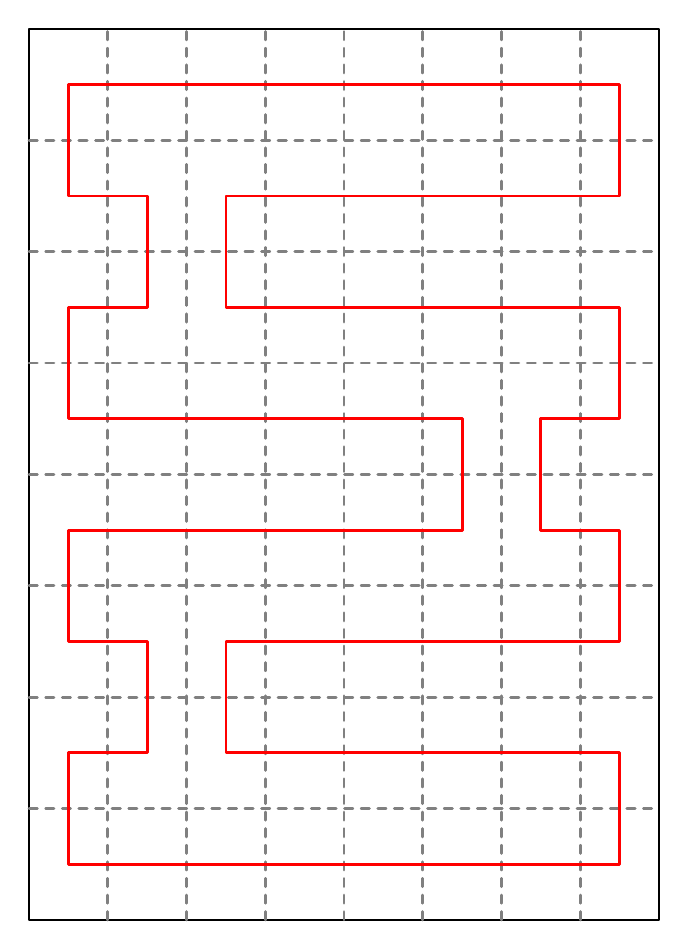
\begin{tikzpicture}[x=1.0cm,y=1.4142135623730951cm,line width=1pt,line cap=round,line join=round]
\draw (0,0) rectangle (8,8);
\draw[dashed,gray] (1,0) -- (1,8) (2,0) -- (2,8) (3,0) -- (3,8) (4,0) -- (4,8) (5,0) -- (5,8) (6,0) -- (6,8) (7,0) -- (7,8) (0,1) -- (8,1) (0,2) -- (8,2) (0,3) -- (8,3) (0,4) -- (8,4) (0,5) -- (8,5) (0,6) -- (8,6) (0,7) -- (8,7);
\draw[red] (0.5,0.5) -- (1.5,0.5) -- (2.5,0.5) -- (3.5,0.5) -- (4.5,0.5) -- (5.5,0.5) -- (6.5,0.5) -- (7.5,0.5) -- (7.5,1.5) -- (6.5,1.5) -- (5.5,1.5) -- (4.5,1.5) -- (3.5,1.5) -- (2.5,1.5) -- (2.5,2.5) -- (3.5,2.5) -- (4.5,2.5) -- (5.5,2.5) -- (6.5,2.5) -- (7.5,2.5) -- (7.5,3.5) -- (6.5,3.5) -- (6.5,4.5) -- (7.5,4.5) -- (7.5,5.5) -- (6.5,5.5) -- (5.5,5.5) -- (4.5,5.5) -- (3.5,5.5) -- (2.5,5.5) -- (2.5,6.5) -- (3.5,6.5) -- (4.5,6.5) -- (5.5,6.5) -- (6.5,6.5) -- (7.5,6.5) -- (7.5,7.5) -- (6.5,7.5) -- (5.5,7.5) -- (4.5,7.5) -- (3.5,7.5) -- (2.5,7.5) -- (1.5,7.5) -- (0.5,7.5) -- (0.5,6.5) -- (1.5,6.5) -- (1.5,5.5) -- (0.5,5.5) -- (0.5,4.5) -- (1.5,4.5) -- (2.5,4.5) -- (3.5,4.5) -- (4.5,4.5) -- (5.5,4.5) -- (5.5,3.5) -- (4.5,3.5) -- (3.5,3.5) -- (2.5,3.5) -- (1.5,3.5) -- (0.5,3.5) -- (0.5,2.5) -- (1.5,2.5) -- (1.5,1.5) -- (0.5,1.5) -- (0.5,0.5) -- cycle;\end{tikzpicture}

\vspace{5mm}

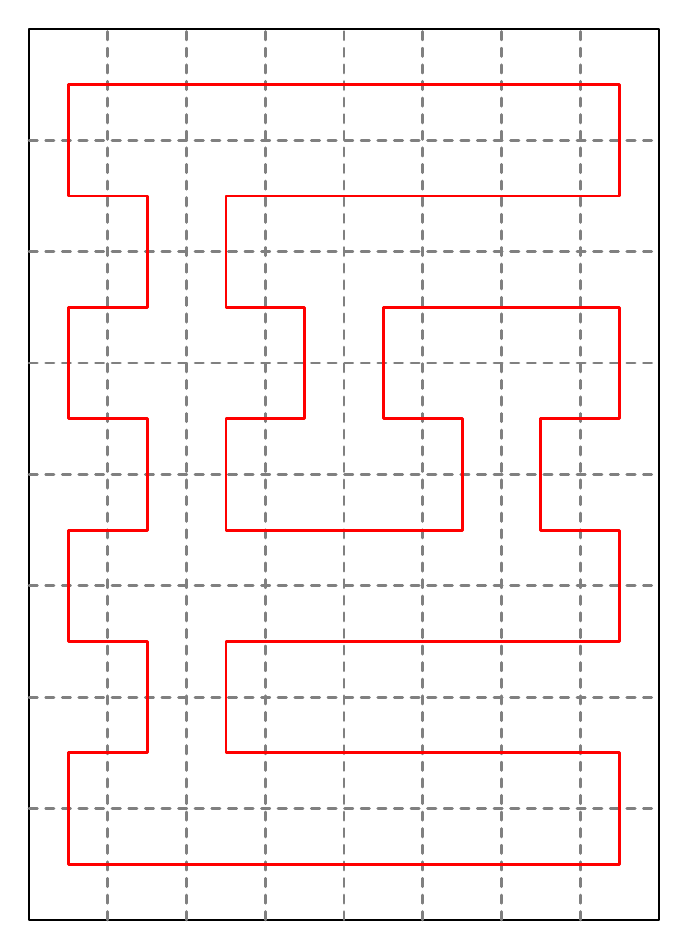
\begin{tikzpicture}[x=1.0cm,y=1.4142135623730951cm,line width=1pt,line cap=round,line join=round]
\draw (0,0) rectangle (8,8);
\draw[dashed,gray] (1,0) -- (1,8) (2,0) -- (2,8) (3,0) -- (3,8) (4,0) -- (4,8) (5,0) -- (5,8) (6,0) -- (6,8) (7,0) -- (7,8) (0,1) -- (8,1) (0,2) -- (8,2) (0,3) -- (8,3) (0,4) -- (8,4) (0,5) -- (8,5) (0,6) -- (8,6) (0,7) -- (8,7);
\draw[red] (0.5,0.5) -- (1.5,0.5) -- (2.5,0.5) -- (3.5,0.5) -- (4.5,0.5) -- (5.5,0.5) -- (6.5,0.5) -- (7.5,0.5) -- (7.5,1.5) -- (6.5,1.5) -- (5.5,1.5) -- (4.5,1.5) -- (3.5,1.5) -- (2.5,1.5) -- (2.5,2.5) -- (3.5,2.5) -- (4.5,2.5) -- (5.5,2.5) -- (6.5,2.5) -- (7.5,2.5) -- (7.5,3.5) -- (6.5,3.5) -- (6.5,4.5) -- (7.5,4.5) -- (7.5,5.5) -- (6.5,5.5) -- (5.5,5.5) -- (4.5,5.5) -- (4.5,4.5) -- (5.5,4.5) -- (5.5,3.5) -- (4.5,3.5) -- (3.5,3.5) -- (2.5,3.5) -- (2.5,4.5) -- (3.5,4.5) -- (3.5,5.5) -- (2.5,5.5) -- (2.5,6.5) -- (3.5,6.5) -- (4.5,6.5) -- (5.5,6.5) -- (6.5,6.5) -- (7.5,6.5) -- (7.5,7.5) -- (6.5,7.5) -- (5.5,7.5) -- (4.5,7.5) -- (3.5,7.5) -- (2.5,7.5) -- (1.5,7.5) -- (0.5,7.5) -- (0.5,6.5) -- (1.5,6.5) -- (1.5,5.5) -- (0.5,5.5) -- (0.5,4.5) -- (1.5,4.5) -- (1.5,3.5) -- (0.5,3.5) -- (0.5,2.5) -- (1.5,2.5) -- (1.5,1.5) -- (0.5,1.5) -- (0.5,0.5) -- cycle;\end{tikzpicture}
\hspace{5mm}
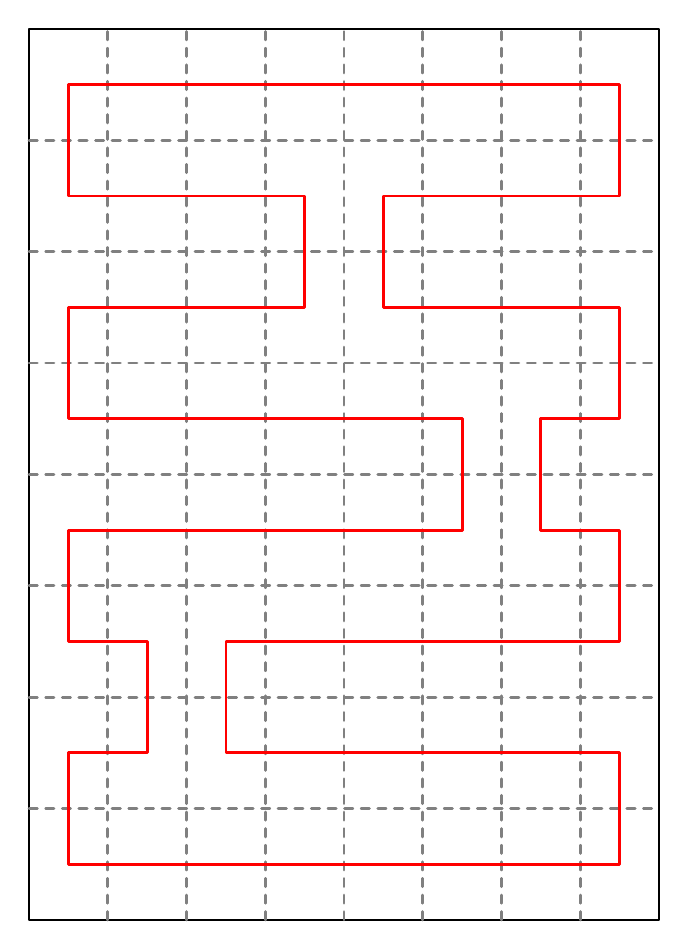
\begin{tikzpicture}[x=1.0cm,y=1.4142135623730951cm,line width=1pt,line cap=round,line join=round]
\draw (0,0) rectangle (8,8);
\draw[dashed,gray] (1,0) -- (1,8) (2,0) -- (2,8) (3,0) -- (3,8) (4,0) -- (4,8) (5,0) -- (5,8) (6,0) -- (6,8) (7,0) -- (7,8) (0,1) -- (8,1) (0,2) -- (8,2) (0,3) -- (8,3) (0,4) -- (8,4) (0,5) -- (8,5) (0,6) -- (8,6) (0,7) -- (8,7);
\draw[red] (0.5,0.5) -- (1.5,0.5) -- (2.5,0.5) -- (3.5,0.5) -- (4.5,0.5) -- (5.5,0.5) -- (6.5,0.5) -- (7.5,0.5) -- (7.5,1.5) -- (6.5,1.5) -- (5.5,1.5) -- (4.5,1.5) -- (3.5,1.5) -- (2.5,1.5) -- (2.5,2.5) -- (3.5,2.5) -- (4.5,2.5) -- (5.5,2.5) -- (6.5,2.5) -- (7.5,2.5) -- (7.5,3.5) -- (6.5,3.5) -- (6.5,4.5) -- (7.5,4.5) -- (7.5,5.5) -- (6.5,5.5) -- (5.5,5.5) -- (4.5,5.5) -- (4.5,6.5) -- (5.5,6.5) -- (6.5,6.5) -- (7.5,6.5) -- (7.5,7.5) -- (6.5,7.5) -- (5.5,7.5) -- (4.5,7.5) -- (3.5,7.5) -- (2.5,7.5) -- (1.5,7.5) -- (0.5,7.5) -- (0.5,6.5) -- (1.5,6.5) -- (2.5,6.5) -- (3.5,6.5) -- (3.5,5.5) -- (2.5,5.5) -- (1.5,5.5) -- (0.5,5.5) -- (0.5,4.5) -- (1.5,4.5) -- (2.5,4.5) -- (3.5,4.5) -- (4.5,4.5) -- (5.5,4.5) -- (5.5,3.5) -- (4.5,3.5) -- (3.5,3.5) -- (2.5,3.5) -- (1.5,3.5) -- (0.5,3.5) -- (0.5,2.5) -- (1.5,2.5) -- (1.5,1.5) -- (0.5,1.5) -- (0.5,0.5) -- cycle;\end{tikzpicture}

\vspace{5mm}

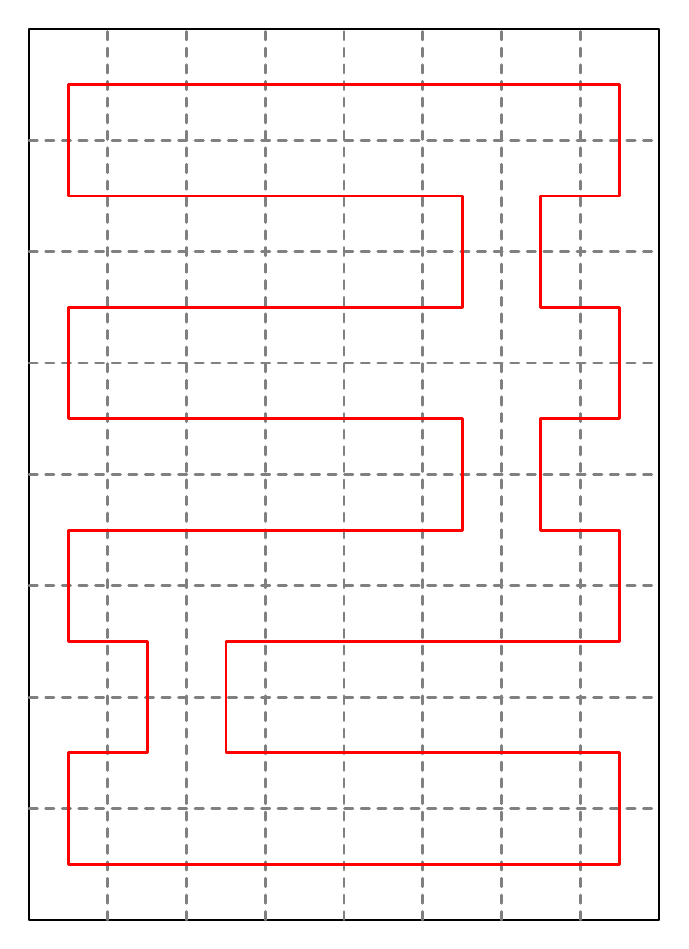
\begin{tikzpicture}[x=1.0cm,y=1.4142135623730951cm,line width=1pt,line cap=round,line join=round]
\draw (0,0) rectangle (8,8);
\draw[dashed,gray] (1,0) -- (1,8) (2,0) -- (2,8) (3,0) -- (3,8) (4,0) -- (4,8) (5,0) -- (5,8) (6,0) -- (6,8) (7,0) -- (7,8) (0,1) -- (8,1) (0,2) -- (8,2) (0,3) -- (8,3) (0,4) -- (8,4) (0,5) -- (8,5) (0,6) -- (8,6) (0,7) -- (8,7);
\draw[red] (0.5,0.5) -- (1.5,0.5) -- (2.5,0.5) -- (3.5,0.5) -- (4.5,0.5) -- (5.5,0.5) -- (6.5,0.5) -- (7.5,0.5) -- (7.5,1.5) -- (6.5,1.5) -- (5.5,1.5) -- (4.5,1.5) -- (3.5,1.5) -- (2.5,1.5) -- (2.5,2.5) -- (3.5,2.5) -- (4.5,2.5) -- (5.5,2.5) -- (6.5,2.5) -- (7.5,2.5) -- (7.5,3.5) -- (6.5,3.5) -- (6.5,4.5) -- (7.5,4.5) -- (7.5,5.5) -- (6.5,5.5) -- (6.5,6.5) -- (7.5,6.5) -- (7.5,7.5) -- (6.5,7.5) -- (5.5,7.5) -- (4.5,7.5) -- (3.5,7.5) -- (2.5,7.5) -- (1.5,7.5) -- (0.5,7.5) -- (0.5,6.5) -- (1.5,6.5) -- (2.5,6.5) -- (3.5,6.5) -- (4.5,6.5) -- (5.5,6.5) -- (5.5,5.5) -- (4.5,5.5) -- (3.5,5.5) -- (2.5,5.5) -- (1.5,5.5) -- (0.5,5.5) -- (0.5,4.5) -- (1.5,4.5) -- (2.5,4.5) -- (3.5,4.5) -- (4.5,4.5) -- (5.5,4.5) -- (5.5,3.5) -- (4.5,3.5) -- (3.5,3.5) -- (2.5,3.5) -- (1.5,3.5) -- (0.5,3.5) -- (0.5,2.5) -- (1.5,2.5) -- (1.5,1.5) -- (0.5,1.5) -- (0.5,0.5) -- cycle;\end{tikzpicture}
\hspace{5mm}
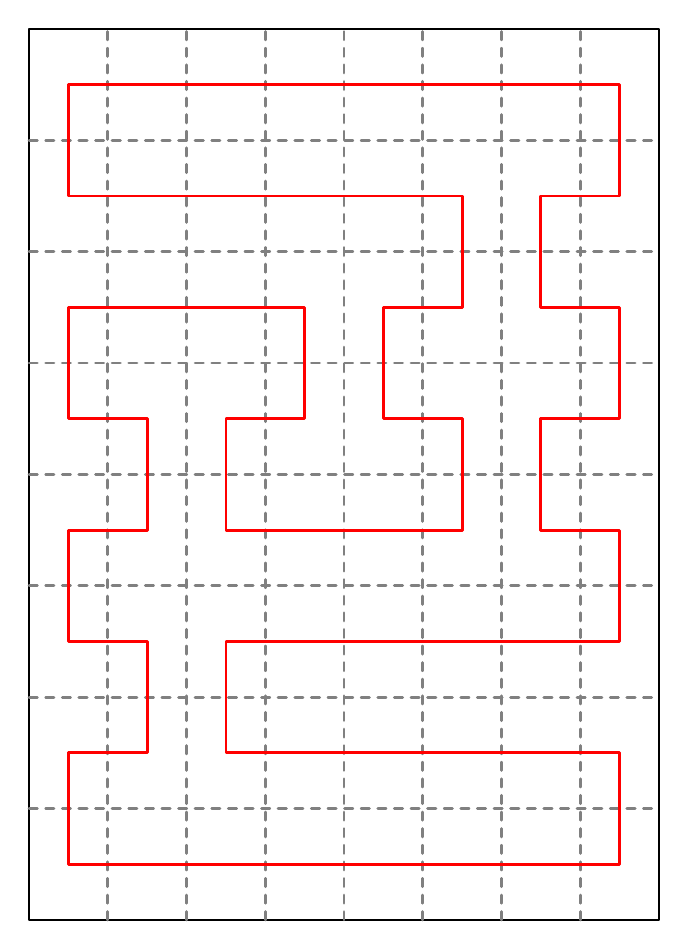
\begin{tikzpicture}[x=1.0cm,y=1.4142135623730951cm,line width=1pt,line cap=round,line join=round]
\draw (0,0) rectangle (8,8);
\draw[dashed,gray] (1,0) -- (1,8) (2,0) -- (2,8) (3,0) -- (3,8) (4,0) -- (4,8) (5,0) -- (5,8) (6,0) -- (6,8) (7,0) -- (7,8) (0,1) -- (8,1) (0,2) -- (8,2) (0,3) -- (8,3) (0,4) -- (8,4) (0,5) -- (8,5) (0,6) -- (8,6) (0,7) -- (8,7);
\draw[red] (0.5,0.5) -- (1.5,0.5) -- (2.5,0.5) -- (3.5,0.5) -- (4.5,0.5) -- (5.5,0.5) -- (6.5,0.5) -- (7.5,0.5) -- (7.5,1.5) -- (6.5,1.5) -- (5.5,1.5) -- (4.5,1.5) -- (3.5,1.5) -- (2.5,1.5) -- (2.5,2.5) -- (3.5,2.5) -- (4.5,2.5) -- (5.5,2.5) -- (6.5,2.5) -- (7.5,2.5) -- (7.5,3.5) -- (6.5,3.5) -- (6.5,4.5) -- (7.5,4.5) -- (7.5,5.5) -- (6.5,5.5) -- (6.5,6.5) -- (7.5,6.5) -- (7.5,7.5) -- (6.5,7.5) -- (5.5,7.5) -- (4.5,7.5) -- (3.5,7.5) -- (2.5,7.5) -- (1.5,7.5) -- (0.5,7.5) -- (0.5,6.5) -- (1.5,6.5) -- (2.5,6.5) -- (3.5,6.5) -- (4.5,6.5) -- (5.5,6.5) -- (5.5,5.5) -- (4.5,5.5) -- (4.5,4.5) -- (5.5,4.5) -- (5.5,3.5) -- (4.5,3.5) -- (3.5,3.5) -- (2.5,3.5) -- (2.5,4.5) -- (3.5,4.5) -- (3.5,5.5) -- (2.5,5.5) -- (1.5,5.5) -- (0.5,5.5) -- (0.5,4.5) -- (1.5,4.5) -- (1.5,3.5) -- (0.5,3.5) -- (0.5,2.5) -- (1.5,2.5) -- (1.5,1.5) -- (0.5,1.5) -- (0.5,0.5) -- cycle;\end{tikzpicture}

\vspace{5mm}

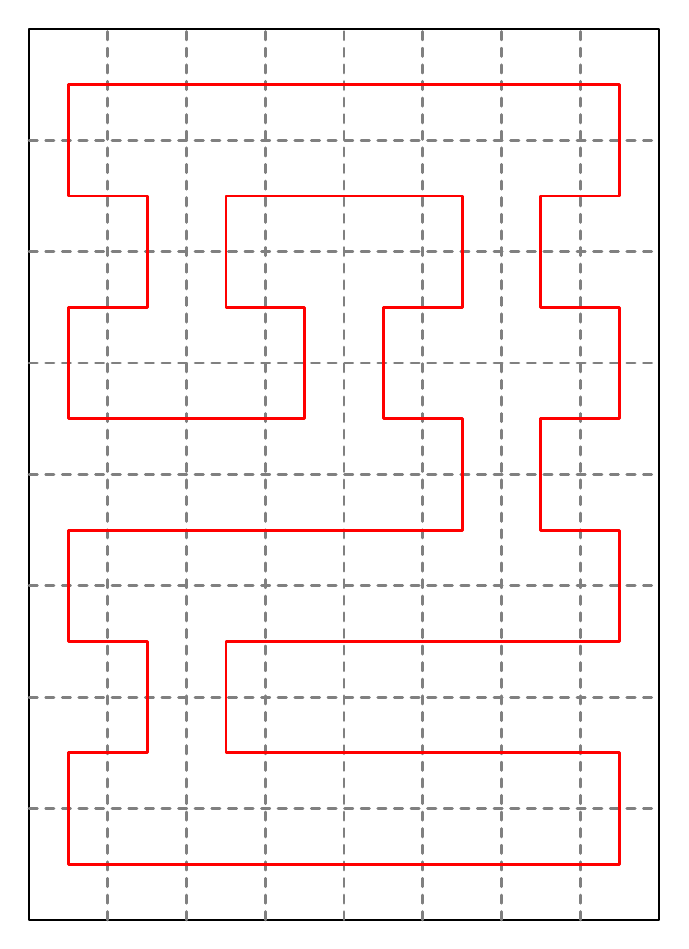
\begin{tikzpicture}[x=1.0cm,y=1.4142135623730951cm,line width=1pt,line cap=round,line join=round]
\draw (0,0) rectangle (8,8);
\draw[dashed,gray] (1,0) -- (1,8) (2,0) -- (2,8) (3,0) -- (3,8) (4,0) -- (4,8) (5,0) -- (5,8) (6,0) -- (6,8) (7,0) -- (7,8) (0,1) -- (8,1) (0,2) -- (8,2) (0,3) -- (8,3) (0,4) -- (8,4) (0,5) -- (8,5) (0,6) -- (8,6) (0,7) -- (8,7);
\draw[red] (0.5,0.5) -- (1.5,0.5) -- (2.5,0.5) -- (3.5,0.5) -- (4.5,0.5) -- (5.5,0.5) -- (6.5,0.5) -- (7.5,0.5) -- (7.5,1.5) -- (6.5,1.5) -- (5.5,1.5) -- (4.5,1.5) -- (3.5,1.5) -- (2.5,1.5) -- (2.5,2.5) -- (3.5,2.5) -- (4.5,2.5) -- (5.5,2.5) -- (6.5,2.5) -- (7.5,2.5) -- (7.5,3.5) -- (6.5,3.5) -- (6.5,4.5) -- (7.5,4.5) -- (7.5,5.5) -- (6.5,5.5) -- (6.5,6.5) -- (7.5,6.5) -- (7.5,7.5) -- (6.5,7.5) -- (5.5,7.5) -- (4.5,7.5) -- (3.5,7.5) -- (2.5,7.5) -- (1.5,7.5) -- (0.5,7.5) -- (0.5,6.5) -- (1.5,6.5) -- (1.5,5.5) -- (0.5,5.5) -- (0.5,4.5) -- (1.5,4.5) -- (2.5,4.5) -- (3.5,4.5) -- (3.5,5.5) -- (2.5,5.5) -- (2.5,6.5) -- (3.5,6.5) -- (4.5,6.5) -- (5.5,6.5) -- (5.5,5.5) -- (4.5,5.5) -- (4.5,4.5) -- (5.5,4.5) -- (5.5,3.5) -- (4.5,3.5) -- (3.5,3.5) -- (2.5,3.5) -- (1.5,3.5) -- (0.5,3.5) -- (0.5,2.5) -- (1.5,2.5) -- (1.5,1.5) -- (0.5,1.5) -- (0.5,0.5) -- cycle;\end{tikzpicture}
\hspace{5mm}
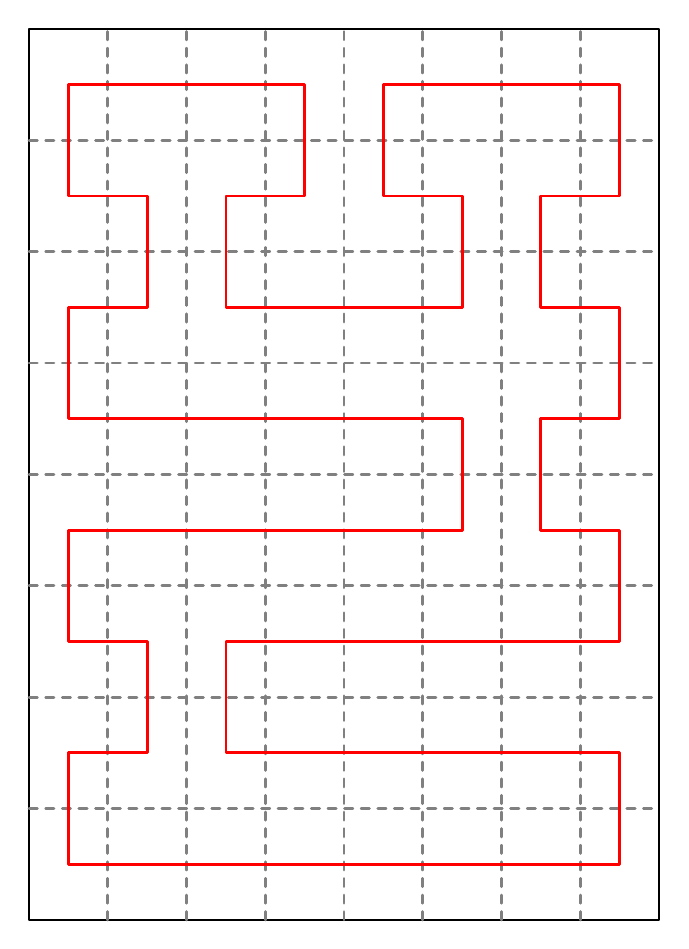
\begin{tikzpicture}[x=1.0cm,y=1.4142135623730951cm,line width=1pt,line cap=round,line join=round]
\draw (0,0) rectangle (8,8);
\draw[dashed,gray] (1,0) -- (1,8) (2,0) -- (2,8) (3,0) -- (3,8) (4,0) -- (4,8) (5,0) -- (5,8) (6,0) -- (6,8) (7,0) -- (7,8) (0,1) -- (8,1) (0,2) -- (8,2) (0,3) -- (8,3) (0,4) -- (8,4) (0,5) -- (8,5) (0,6) -- (8,6) (0,7) -- (8,7);
\draw[red] (0.5,0.5) -- (1.5,0.5) -- (2.5,0.5) -- (3.5,0.5) -- (4.5,0.5) -- (5.5,0.5) -- (6.5,0.5) -- (7.5,0.5) -- (7.5,1.5) -- (6.5,1.5) -- (5.5,1.5) -- (4.5,1.5) -- (3.5,1.5) -- (2.5,1.5) -- (2.5,2.5) -- (3.5,2.5) -- (4.5,2.5) -- (5.5,2.5) -- (6.5,2.5) -- (7.5,2.5) -- (7.5,3.5) -- (6.5,3.5) -- (6.5,4.5) -- (7.5,4.5) -- (7.5,5.5) -- (6.5,5.5) -- (6.5,6.5) -- (7.5,6.5) -- (7.5,7.5) -- (6.5,7.5) -- (5.5,7.5) -- (4.5,7.5) -- (4.5,6.5) -- (5.5,6.5) -- (5.5,5.5) -- (4.5,5.5) -- (3.5,5.5) -- (2.5,5.5) -- (2.5,6.5) -- (3.5,6.5) -- (3.5,7.5) -- (2.5,7.5) -- (1.5,7.5) -- (0.5,7.5) -- (0.5,6.5) -- (1.5,6.5) -- (1.5,5.5) -- (0.5,5.5) -- (0.5,4.5) -- (1.5,4.5) -- (2.5,4.5) -- (3.5,4.5) -- (4.5,4.5) -- (5.5,4.5) -- (5.5,3.5) -- (4.5,3.5) -- (3.5,3.5) -- (2.5,3.5) -- (1.5,3.5) -- (0.5,3.5) -- (0.5,2.5) -- (1.5,2.5) -- (1.5,1.5) -- (0.5,1.5) -- (0.5,0.5) -- cycle;\end{tikzpicture}

\vspace{5mm}

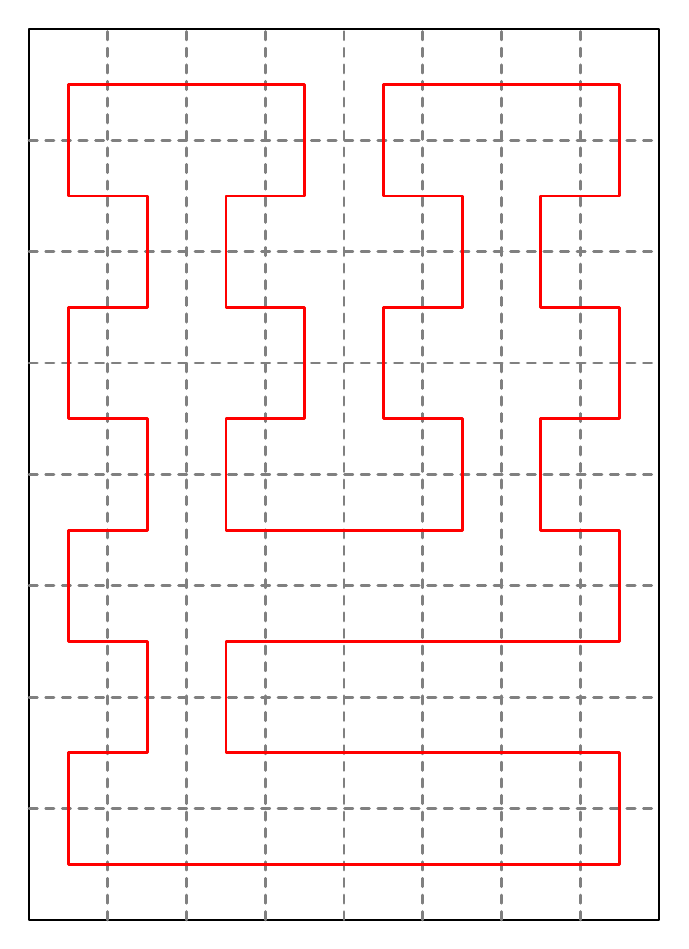
\begin{tikzpicture}[x=1.0cm,y=1.4142135623730951cm,line width=1pt,line cap=round,line join=round]
\draw (0,0) rectangle (8,8);
\draw[dashed,gray] (1,0) -- (1,8) (2,0) -- (2,8) (3,0) -- (3,8) (4,0) -- (4,8) (5,0) -- (5,8) (6,0) -- (6,8) (7,0) -- (7,8) (0,1) -- (8,1) (0,2) -- (8,2) (0,3) -- (8,3) (0,4) -- (8,4) (0,5) -- (8,5) (0,6) -- (8,6) (0,7) -- (8,7);
\draw[red] (0.5,0.5) -- (1.5,0.5) -- (2.5,0.5) -- (3.5,0.5) -- (4.5,0.5) -- (5.5,0.5) -- (6.5,0.5) -- (7.5,0.5) -- (7.5,1.5) -- (6.5,1.5) -- (5.5,1.5) -- (4.5,1.5) -- (3.5,1.5) -- (2.5,1.5) -- (2.5,2.5) -- (3.5,2.5) -- (4.5,2.5) -- (5.5,2.5) -- (6.5,2.5) -- (7.5,2.5) -- (7.5,3.5) -- (6.5,3.5) -- (6.5,4.5) -- (7.5,4.5) -- (7.5,5.5) -- (6.5,5.5) -- (6.5,6.5) -- (7.5,6.5) -- (7.5,7.5) -- (6.5,7.5) -- (5.5,7.5) -- (4.5,7.5) -- (4.5,6.5) -- (5.5,6.5) -- (5.5,5.5) -- (4.5,5.5) -- (4.5,4.5) -- (5.5,4.5) -- (5.5,3.5) -- (4.5,3.5) -- (3.5,3.5) -- (2.5,3.5) -- (2.5,4.5) -- (3.5,4.5) -- (3.5,5.5) -- (2.5,5.5) -- (2.5,6.5) -- (3.5,6.5) -- (3.5,7.5) -- (2.5,7.5) -- (1.5,7.5) -- (0.5,7.5) -- (0.5,6.5) -- (1.5,6.5) -- (1.5,5.5) -- (0.5,5.5) -- (0.5,4.5) -- (1.5,4.5) -- (1.5,3.5) -- (0.5,3.5) -- (0.5,2.5) -- (1.5,2.5) -- (1.5,1.5) -- (0.5,1.5) -- (0.5,0.5) -- cycle;\end{tikzpicture}
\hspace{5mm}
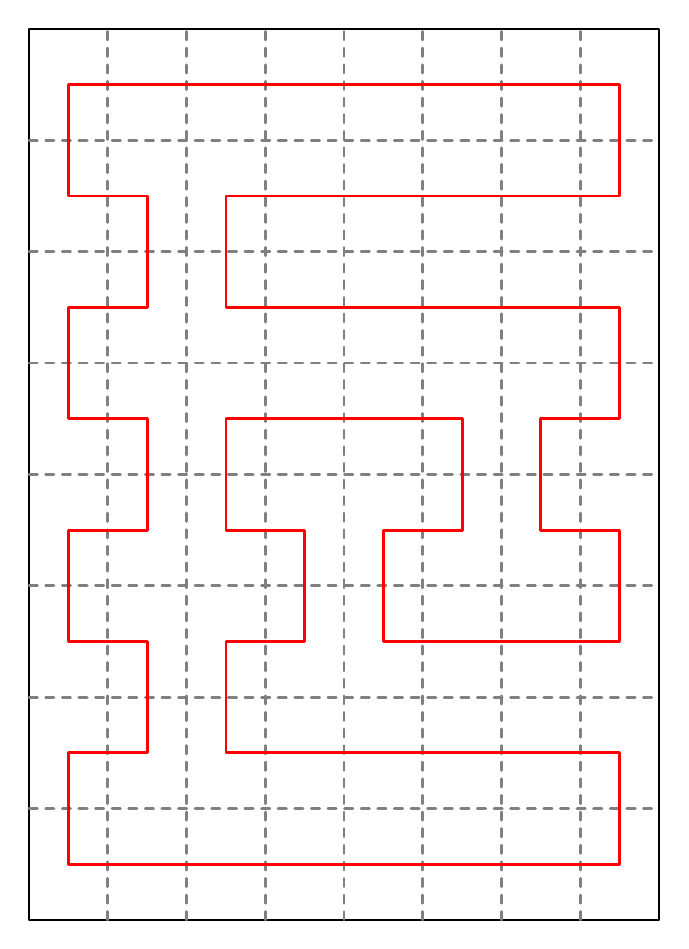
\begin{tikzpicture}[x=1.0cm,y=1.4142135623730951cm,line width=1pt,line cap=round,line join=round]
\draw (0,0) rectangle (8,8);
\draw[dashed,gray] (1,0) -- (1,8) (2,0) -- (2,8) (3,0) -- (3,8) (4,0) -- (4,8) (5,0) -- (5,8) (6,0) -- (6,8) (7,0) -- (7,8) (0,1) -- (8,1) (0,2) -- (8,2) (0,3) -- (8,3) (0,4) -- (8,4) (0,5) -- (8,5) (0,6) -- (8,6) (0,7) -- (8,7);
\draw[red] (0.5,0.5) -- (1.5,0.5) -- (2.5,0.5) -- (3.5,0.5) -- (4.5,0.5) -- (5.5,0.5) -- (6.5,0.5) -- (7.5,0.5) -- (7.5,1.5) -- (6.5,1.5) -- (5.5,1.5) -- (4.5,1.5) -- (3.5,1.5) -- (2.5,1.5) -- (2.5,2.5) -- (3.5,2.5) -- (3.5,3.5) -- (2.5,3.5) -- (2.5,4.5) -- (3.5,4.5) -- (4.5,4.5) -- (5.5,4.5) -- (5.5,3.5) -- (4.5,3.5) -- (4.5,2.5) -- (5.5,2.5) -- (6.5,2.5) -- (7.5,2.5) -- (7.5,3.5) -- (6.5,3.5) -- (6.5,4.5) -- (7.5,4.5) -- (7.5,5.5) -- (6.5,5.5) -- (5.5,5.5) -- (4.5,5.5) -- (3.5,5.5) -- (2.5,5.5) -- (2.5,6.5) -- (3.5,6.5) -- (4.5,6.5) -- (5.5,6.5) -- (6.5,6.5) -- (7.5,6.5) -- (7.5,7.5) -- (6.5,7.5) -- (5.5,7.5) -- (4.5,7.5) -- (3.5,7.5) -- (2.5,7.5) -- (1.5,7.5) -- (0.5,7.5) -- (0.5,6.5) -- (1.5,6.5) -- (1.5,5.5) -- (0.5,5.5) -- (0.5,4.5) -- (1.5,4.5) -- (1.5,3.5) -- (0.5,3.5) -- (0.5,2.5) -- (1.5,2.5) -- (1.5,1.5) -- (0.5,1.5) -- (0.5,0.5) -- cycle;\end{tikzpicture}

\vspace{5mm}

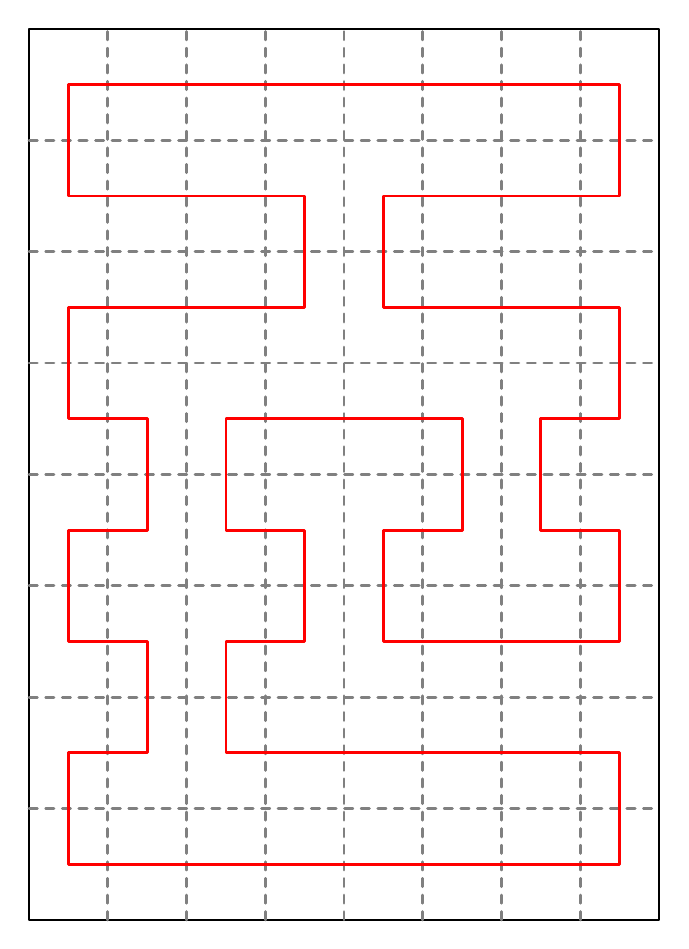
\begin{tikzpicture}[x=1.0cm,y=1.4142135623730951cm,line width=1pt,line cap=round,line join=round]
\draw (0,0) rectangle (8,8);
\draw[dashed,gray] (1,0) -- (1,8) (2,0) -- (2,8) (3,0) -- (3,8) (4,0) -- (4,8) (5,0) -- (5,8) (6,0) -- (6,8) (7,0) -- (7,8) (0,1) -- (8,1) (0,2) -- (8,2) (0,3) -- (8,3) (0,4) -- (8,4) (0,5) -- (8,5) (0,6) -- (8,6) (0,7) -- (8,7);
\draw[red] (0.5,0.5) -- (1.5,0.5) -- (2.5,0.5) -- (3.5,0.5) -- (4.5,0.5) -- (5.5,0.5) -- (6.5,0.5) -- (7.5,0.5) -- (7.5,1.5) -- (6.5,1.5) -- (5.5,1.5) -- (4.5,1.5) -- (3.5,1.5) -- (2.5,1.5) -- (2.5,2.5) -- (3.5,2.5) -- (3.5,3.5) -- (2.5,3.5) -- (2.5,4.5) -- (3.5,4.5) -- (4.5,4.5) -- (5.5,4.5) -- (5.5,3.5) -- (4.5,3.5) -- (4.5,2.5) -- (5.5,2.5) -- (6.5,2.5) -- (7.5,2.5) -- (7.5,3.5) -- (6.5,3.5) -- (6.5,4.5) -- (7.5,4.5) -- (7.5,5.5) -- (6.5,5.5) -- (5.5,5.5) -- (4.5,5.5) -- (4.5,6.5) -- (5.5,6.5) -- (6.5,6.5) -- (7.5,6.5) -- (7.5,7.5) -- (6.5,7.5) -- (5.5,7.5) -- (4.5,7.5) -- (3.5,7.5) -- (2.5,7.5) -- (1.5,7.5) -- (0.5,7.5) -- (0.5,6.5) -- (1.5,6.5) -- (2.5,6.5) -- (3.5,6.5) -- (3.5,5.5) -- (2.5,5.5) -- (1.5,5.5) -- (0.5,5.5) -- (0.5,4.5) -- (1.5,4.5) -- (1.5,3.5) -- (0.5,3.5) -- (0.5,2.5) -- (1.5,2.5) -- (1.5,1.5) -- (0.5,1.5) -- (0.5,0.5) -- cycle;\end{tikzpicture}
\hspace{5mm}
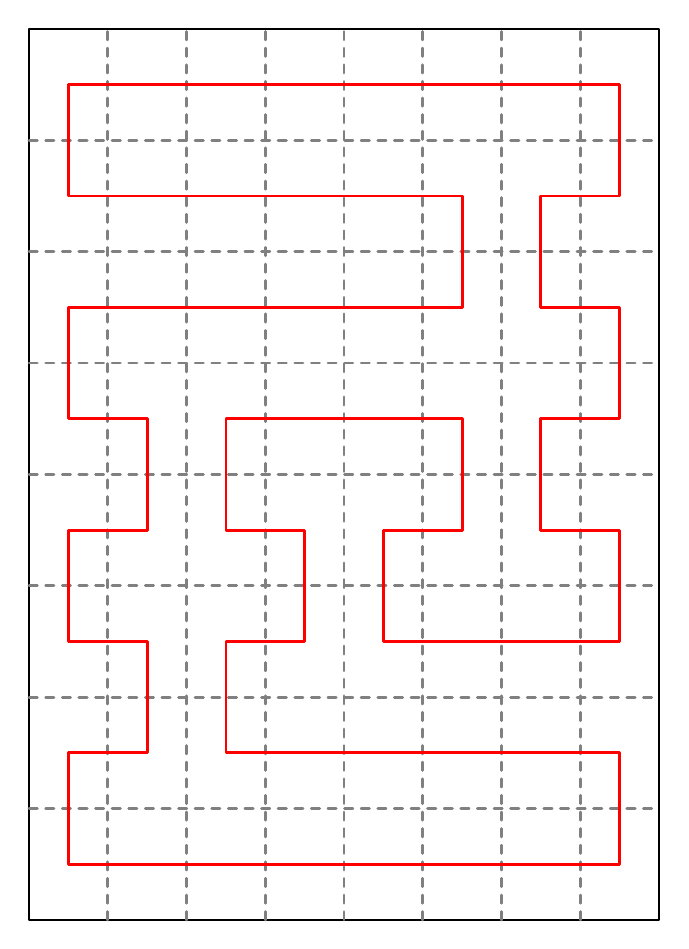
\begin{tikzpicture}[x=1.0cm,y=1.4142135623730951cm,line width=1pt,line cap=round,line join=round]
\draw (0,0) rectangle (8,8);
\draw[dashed,gray] (1,0) -- (1,8) (2,0) -- (2,8) (3,0) -- (3,8) (4,0) -- (4,8) (5,0) -- (5,8) (6,0) -- (6,8) (7,0) -- (7,8) (0,1) -- (8,1) (0,2) -- (8,2) (0,3) -- (8,3) (0,4) -- (8,4) (0,5) -- (8,5) (0,6) -- (8,6) (0,7) -- (8,7);
\draw[red] (0.5,0.5) -- (1.5,0.5) -- (2.5,0.5) -- (3.5,0.5) -- (4.5,0.5) -- (5.5,0.5) -- (6.5,0.5) -- (7.5,0.5) -- (7.5,1.5) -- (6.5,1.5) -- (5.5,1.5) -- (4.5,1.5) -- (3.5,1.5) -- (2.5,1.5) -- (2.5,2.5) -- (3.5,2.5) -- (3.5,3.5) -- (2.5,3.5) -- (2.5,4.5) -- (3.5,4.5) -- (4.5,4.5) -- (5.5,4.5) -- (5.5,3.5) -- (4.5,3.5) -- (4.5,2.5) -- (5.5,2.5) -- (6.5,2.5) -- (7.5,2.5) -- (7.5,3.5) -- (6.5,3.5) -- (6.5,4.5) -- (7.5,4.5) -- (7.5,5.5) -- (6.5,5.5) -- (6.5,6.5) -- (7.5,6.5) -- (7.5,7.5) -- (6.5,7.5) -- (5.5,7.5) -- (4.5,7.5) -- (3.5,7.5) -- (2.5,7.5) -- (1.5,7.5) -- (0.5,7.5) -- (0.5,6.5) -- (1.5,6.5) -- (2.5,6.5) -- (3.5,6.5) -- (4.5,6.5) -- (5.5,6.5) -- (5.5,5.5) -- (4.5,5.5) -- (3.5,5.5) -- (2.5,5.5) -- (1.5,5.5) -- (0.5,5.5) -- (0.5,4.5) -- (1.5,4.5) -- (1.5,3.5) -- (0.5,3.5) -- (0.5,2.5) -- (1.5,2.5) -- (1.5,1.5) -- (0.5,1.5) -- (0.5,0.5) -- cycle;\end{tikzpicture}

\vspace{5mm}

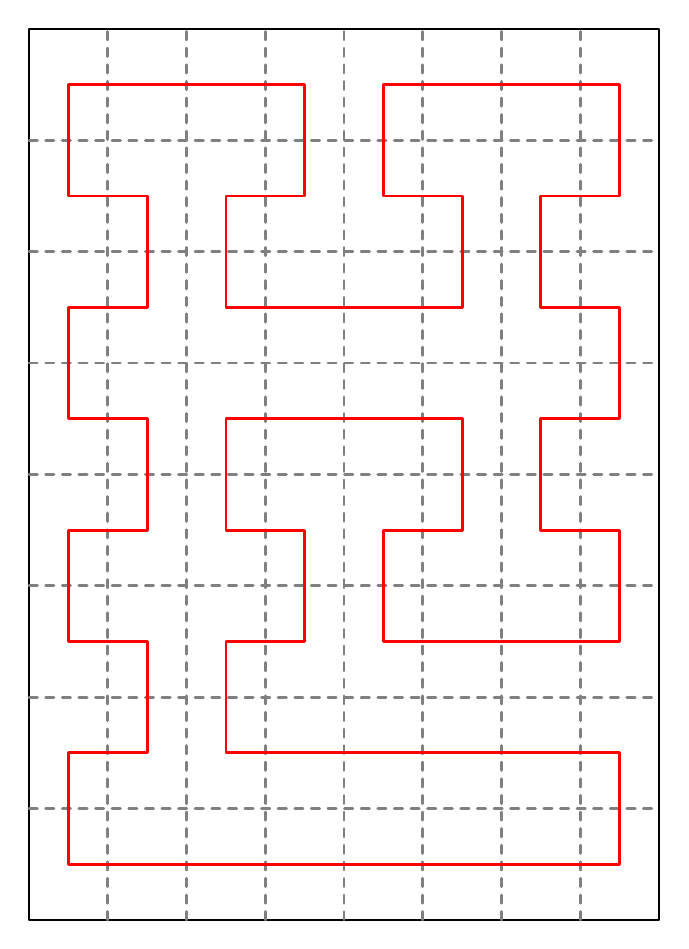
\begin{tikzpicture}[x=1.0cm,y=1.4142135623730951cm,line width=1pt,line cap=round,line join=round]
\draw (0,0) rectangle (8,8);
\draw[dashed,gray] (1,0) -- (1,8) (2,0) -- (2,8) (3,0) -- (3,8) (4,0) -- (4,8) (5,0) -- (5,8) (6,0) -- (6,8) (7,0) -- (7,8) (0,1) -- (8,1) (0,2) -- (8,2) (0,3) -- (8,3) (0,4) -- (8,4) (0,5) -- (8,5) (0,6) -- (8,6) (0,7) -- (8,7);
\draw[red] (0.5,0.5) -- (1.5,0.5) -- (2.5,0.5) -- (3.5,0.5) -- (4.5,0.5) -- (5.5,0.5) -- (6.5,0.5) -- (7.5,0.5) -- (7.5,1.5) -- (6.5,1.5) -- (5.5,1.5) -- (4.5,1.5) -- (3.5,1.5) -- (2.5,1.5) -- (2.5,2.5) -- (3.5,2.5) -- (3.5,3.5) -- (2.5,3.5) -- (2.5,4.5) -- (3.5,4.5) -- (4.5,4.5) -- (5.5,4.5) -- (5.5,3.5) -- (4.5,3.5) -- (4.5,2.5) -- (5.5,2.5) -- (6.5,2.5) -- (7.5,2.5) -- (7.5,3.5) -- (6.5,3.5) -- (6.5,4.5) -- (7.5,4.5) -- (7.5,5.5) -- (6.5,5.5) -- (6.5,6.5) -- (7.5,6.5) -- (7.5,7.5) -- (6.5,7.5) -- (5.5,7.5) -- (4.5,7.5) -- (4.5,6.5) -- (5.5,6.5) -- (5.5,5.5) -- (4.5,5.5) -- (3.5,5.5) -- (2.5,5.5) -- (2.5,6.5) -- (3.5,6.5) -- (3.5,7.5) -- (2.5,7.5) -- (1.5,7.5) -- (0.5,7.5) -- (0.5,6.5) -- (1.5,6.5) -- (1.5,5.5) -- (0.5,5.5) -- (0.5,4.5) -- (1.5,4.5) -- (1.5,3.5) -- (0.5,3.5) -- (0.5,2.5) -- (1.5,2.5) -- (1.5,1.5) -- (0.5,1.5) -- (0.5,0.5) -- cycle;\end{tikzpicture}
\hspace{5mm}
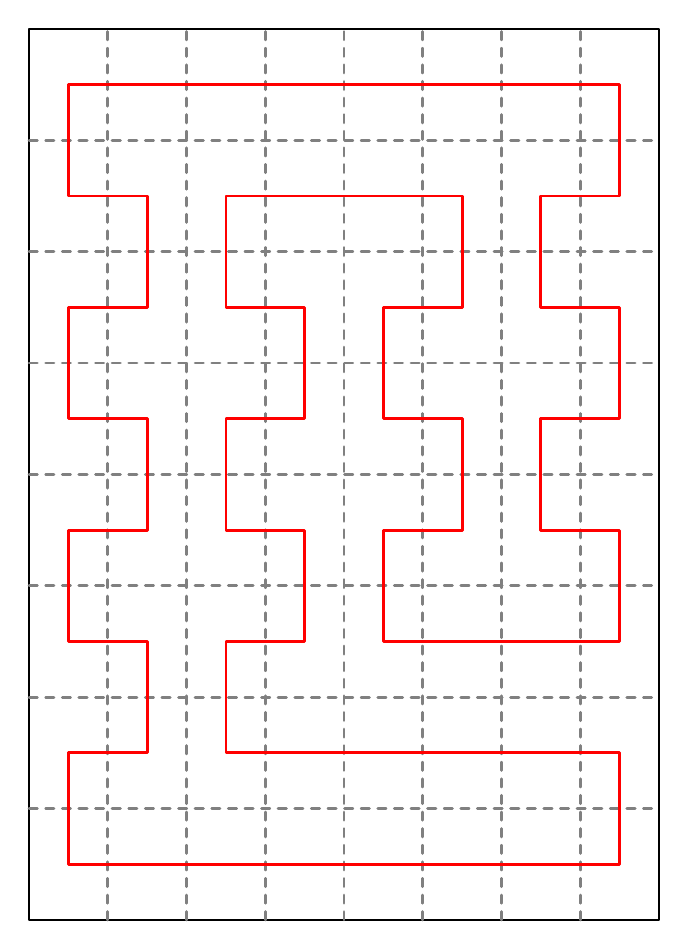
\begin{tikzpicture}[x=1.0cm,y=1.4142135623730951cm,line width=1pt,line cap=round,line join=round]
\draw (0,0) rectangle (8,8);
\draw[dashed,gray] (1,0) -- (1,8) (2,0) -- (2,8) (3,0) -- (3,8) (4,0) -- (4,8) (5,0) -- (5,8) (6,0) -- (6,8) (7,0) -- (7,8) (0,1) -- (8,1) (0,2) -- (8,2) (0,3) -- (8,3) (0,4) -- (8,4) (0,5) -- (8,5) (0,6) -- (8,6) (0,7) -- (8,7);
\draw[red] (0.5,0.5) -- (1.5,0.5) -- (2.5,0.5) -- (3.5,0.5) -- (4.5,0.5) -- (5.5,0.5) -- (6.5,0.5) -- (7.5,0.5) -- (7.5,1.5) -- (6.5,1.5) -- (5.5,1.5) -- (4.5,1.5) -- (3.5,1.5) -- (2.5,1.5) -- (2.5,2.5) -- (3.5,2.5) -- (3.5,3.5) -- (2.5,3.5) -- (2.5,4.5) -- (3.5,4.5) -- (3.5,5.5) -- (2.5,5.5) -- (2.5,6.5) -- (3.5,6.5) -- (4.5,6.5) -- (5.5,6.5) -- (5.5,5.5) -- (4.5,5.5) -- (4.5,4.5) -- (5.5,4.5) -- (5.5,3.5) -- (4.5,3.5) -- (4.5,2.5) -- (5.5,2.5) -- (6.5,2.5) -- (7.5,2.5) -- (7.5,3.5) -- (6.5,3.5) -- (6.5,4.5) -- (7.5,4.5) -- (7.5,5.5) -- (6.5,5.5) -- (6.5,6.5) -- (7.5,6.5) -- (7.5,7.5) -- (6.5,7.5) -- (5.5,7.5) -- (4.5,7.5) -- (3.5,7.5) -- (2.5,7.5) -- (1.5,7.5) -- (0.5,7.5) -- (0.5,6.5) -- (1.5,6.5) -- (1.5,5.5) -- (0.5,5.5) -- (0.5,4.5) -- (1.5,4.5) -- (1.5,3.5) -- (0.5,3.5) -- (0.5,2.5) -- (1.5,2.5) -- (1.5,1.5) -- (0.5,1.5) -- (0.5,0.5) -- cycle;\end{tikzpicture}

\vspace{5mm}

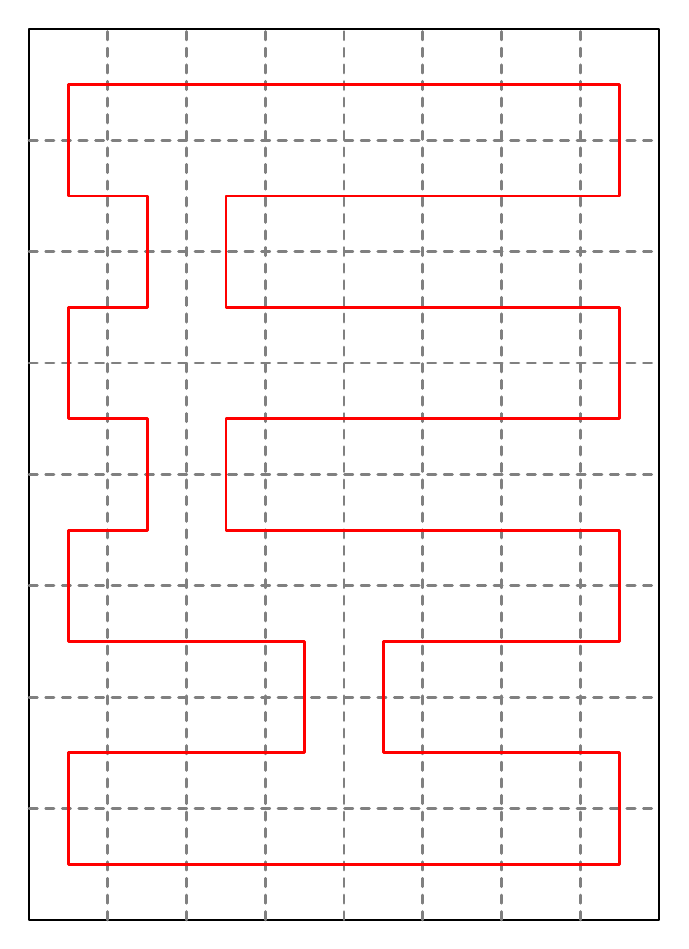
\begin{tikzpicture}[x=1.0cm,y=1.4142135623730951cm,line width=1pt,line cap=round,line join=round]
\draw (0,0) rectangle (8,8);
\draw[dashed,gray] (1,0) -- (1,8) (2,0) -- (2,8) (3,0) -- (3,8) (4,0) -- (4,8) (5,0) -- (5,8) (6,0) -- (6,8) (7,0) -- (7,8) (0,1) -- (8,1) (0,2) -- (8,2) (0,3) -- (8,3) (0,4) -- (8,4) (0,5) -- (8,5) (0,6) -- (8,6) (0,7) -- (8,7);
\draw[red] (0.5,0.5) -- (1.5,0.5) -- (2.5,0.5) -- (3.5,0.5) -- (4.5,0.5) -- (5.5,0.5) -- (6.5,0.5) -- (7.5,0.5) -- (7.5,1.5) -- (6.5,1.5) -- (5.5,1.5) -- (4.5,1.5) -- (4.5,2.5) -- (5.5,2.5) -- (6.5,2.5) -- (7.5,2.5) -- (7.5,3.5) -- (6.5,3.5) -- (5.5,3.5) -- (4.5,3.5) -- (3.5,3.5) -- (2.5,3.5) -- (2.5,4.5) -- (3.5,4.5) -- (4.5,4.5) -- (5.5,4.5) -- (6.5,4.5) -- (7.5,4.5) -- (7.5,5.5) -- (6.5,5.5) -- (5.5,5.5) -- (4.5,5.5) -- (3.5,5.5) -- (2.5,5.5) -- (2.5,6.5) -- (3.5,6.5) -- (4.5,6.5) -- (5.5,6.5) -- (6.5,6.5) -- (7.5,6.5) -- (7.5,7.5) -- (6.5,7.5) -- (5.5,7.5) -- (4.5,7.5) -- (3.5,7.5) -- (2.5,7.5) -- (1.5,7.5) -- (0.5,7.5) -- (0.5,6.5) -- (1.5,6.5) -- (1.5,5.5) -- (0.5,5.5) -- (0.5,4.5) -- (1.5,4.5) -- (1.5,3.5) -- (0.5,3.5) -- (0.5,2.5) -- (1.5,2.5) -- (2.5,2.5) -- (3.5,2.5) -- (3.5,1.5) -- (2.5,1.5) -- (1.5,1.5) -- (0.5,1.5) -- (0.5,0.5) -- cycle;\end{tikzpicture}
\hspace{5mm}
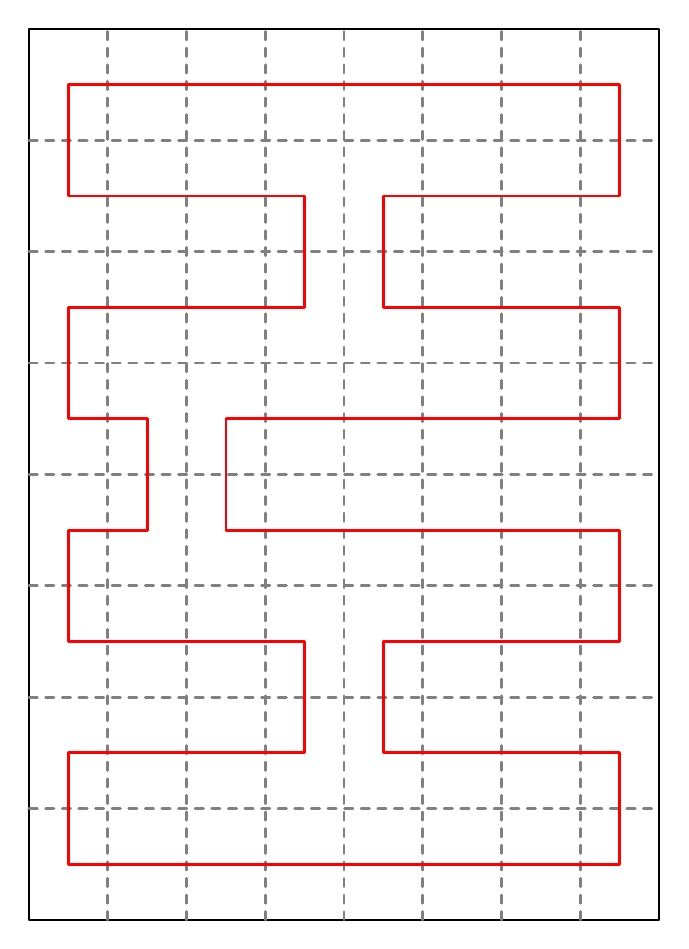
\begin{tikzpicture}[x=1.0cm,y=1.4142135623730951cm,line width=1pt,line cap=round,line join=round]
\draw (0,0) rectangle (8,8);
\draw[dashed,gray] (1,0) -- (1,8) (2,0) -- (2,8) (3,0) -- (3,8) (4,0) -- (4,8) (5,0) -- (5,8) (6,0) -- (6,8) (7,0) -- (7,8) (0,1) -- (8,1) (0,2) -- (8,2) (0,3) -- (8,3) (0,4) -- (8,4) (0,5) -- (8,5) (0,6) -- (8,6) (0,7) -- (8,7);
\draw[red] (0.5,0.5) -- (1.5,0.5) -- (2.5,0.5) -- (3.5,0.5) -- (4.5,0.5) -- (5.5,0.5) -- (6.5,0.5) -- (7.5,0.5) -- (7.5,1.5) -- (6.5,1.5) -- (5.5,1.5) -- (4.5,1.5) -- (4.5,2.5) -- (5.5,2.5) -- (6.5,2.5) -- (7.5,2.5) -- (7.5,3.5) -- (6.5,3.5) -- (5.5,3.5) -- (4.5,3.5) -- (3.5,3.5) -- (2.5,3.5) -- (2.5,4.5) -- (3.5,4.5) -- (4.5,4.5) -- (5.5,4.5) -- (6.5,4.5) -- (7.5,4.5) -- (7.5,5.5) -- (6.5,5.5) -- (5.5,5.5) -- (4.5,5.5) -- (4.5,6.5) -- (5.5,6.5) -- (6.5,6.5) -- (7.5,6.5) -- (7.5,7.5) -- (6.5,7.5) -- (5.5,7.5) -- (4.5,7.5) -- (3.5,7.5) -- (2.5,7.5) -- (1.5,7.5) -- (0.5,7.5) -- (0.5,6.5) -- (1.5,6.5) -- (2.5,6.5) -- (3.5,6.5) -- (3.5,5.5) -- (2.5,5.5) -- (1.5,5.5) -- (0.5,5.5) -- (0.5,4.5) -- (1.5,4.5) -- (1.5,3.5) -- (0.5,3.5) -- (0.5,2.5) -- (1.5,2.5) -- (2.5,2.5) -- (3.5,2.5) -- (3.5,1.5) -- (2.5,1.5) -- (1.5,1.5) -- (0.5,1.5) -- (0.5,0.5) -- cycle;\end{tikzpicture}

\vspace{5mm}

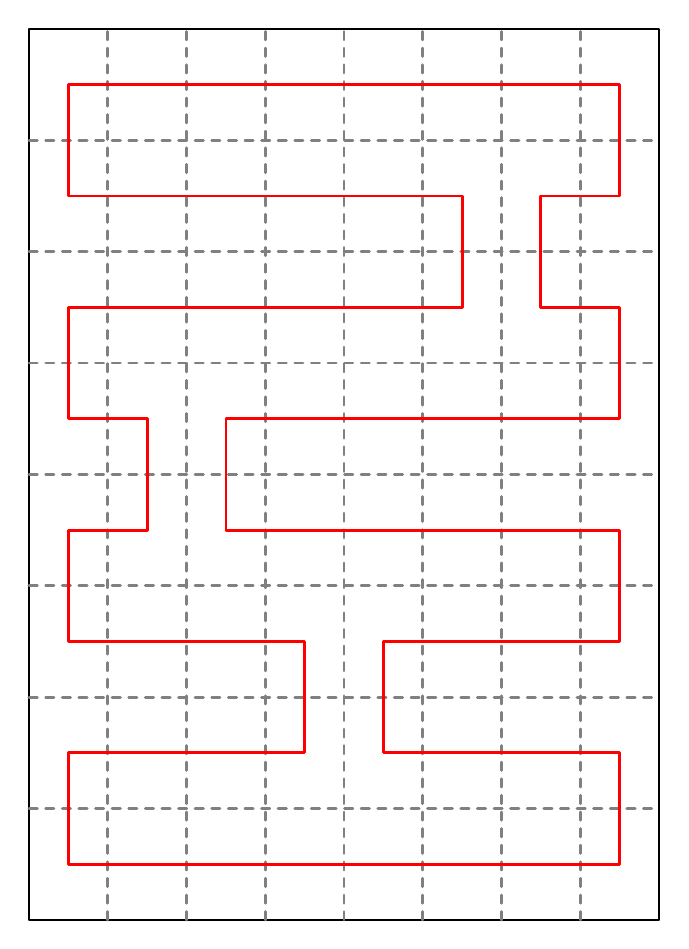
\begin{tikzpicture}[x=1.0cm,y=1.4142135623730951cm,line width=1pt,line cap=round,line join=round]
\draw (0,0) rectangle (8,8);
\draw[dashed,gray] (1,0) -- (1,8) (2,0) -- (2,8) (3,0) -- (3,8) (4,0) -- (4,8) (5,0) -- (5,8) (6,0) -- (6,8) (7,0) -- (7,8) (0,1) -- (8,1) (0,2) -- (8,2) (0,3) -- (8,3) (0,4) -- (8,4) (0,5) -- (8,5) (0,6) -- (8,6) (0,7) -- (8,7);
\draw[red] (0.5,0.5) -- (1.5,0.5) -- (2.5,0.5) -- (3.5,0.5) -- (4.5,0.5) -- (5.5,0.5) -- (6.5,0.5) -- (7.5,0.5) -- (7.5,1.5) -- (6.5,1.5) -- (5.5,1.5) -- (4.5,1.5) -- (4.5,2.5) -- (5.5,2.5) -- (6.5,2.5) -- (7.5,2.5) -- (7.5,3.5) -- (6.5,3.5) -- (5.5,3.5) -- (4.5,3.5) -- (3.5,3.5) -- (2.5,3.5) -- (2.5,4.5) -- (3.5,4.5) -- (4.5,4.5) -- (5.5,4.5) -- (6.5,4.5) -- (7.5,4.5) -- (7.5,5.5) -- (6.5,5.5) -- (6.5,6.5) -- (7.5,6.5) -- (7.5,7.5) -- (6.5,7.5) -- (5.5,7.5) -- (4.5,7.5) -- (3.5,7.5) -- (2.5,7.5) -- (1.5,7.5) -- (0.5,7.5) -- (0.5,6.5) -- (1.5,6.5) -- (2.5,6.5) -- (3.5,6.5) -- (4.5,6.5) -- (5.5,6.5) -- (5.5,5.5) -- (4.5,5.5) -- (3.5,5.5) -- (2.5,5.5) -- (1.5,5.5) -- (0.5,5.5) -- (0.5,4.5) -- (1.5,4.5) -- (1.5,3.5) -- (0.5,3.5) -- (0.5,2.5) -- (1.5,2.5) -- (2.5,2.5) -- (3.5,2.5) -- (3.5,1.5) -- (2.5,1.5) -- (1.5,1.5) -- (0.5,1.5) -- (0.5,0.5) -- cycle;\end{tikzpicture}
\hspace{5mm}
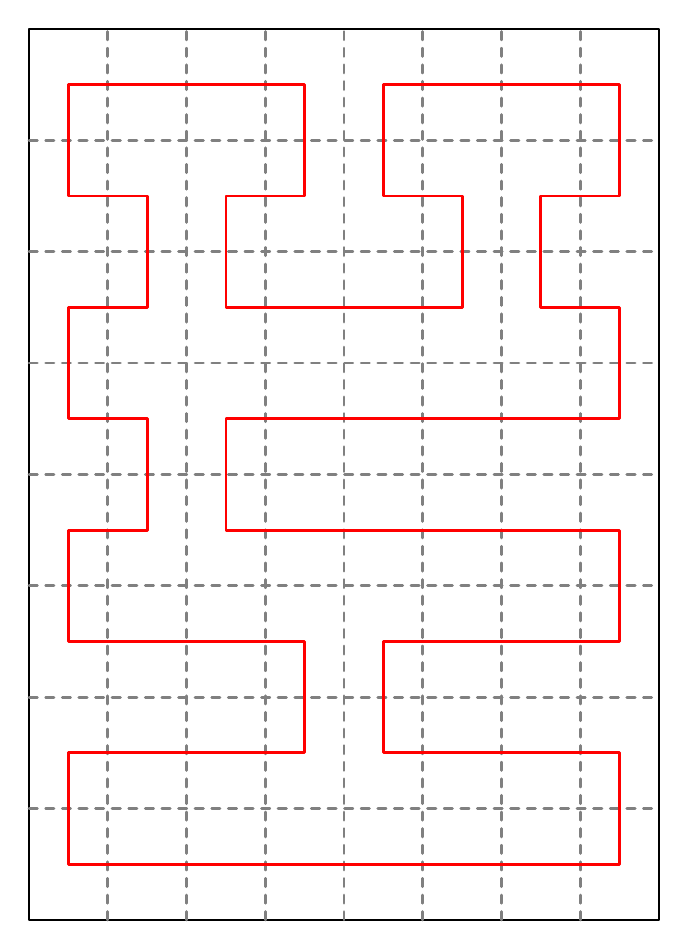
\begin{tikzpicture}[x=1.0cm,y=1.4142135623730951cm,line width=1pt,line cap=round,line join=round]
\draw (0,0) rectangle (8,8);
\draw[dashed,gray] (1,0) -- (1,8) (2,0) -- (2,8) (3,0) -- (3,8) (4,0) -- (4,8) (5,0) -- (5,8) (6,0) -- (6,8) (7,0) -- (7,8) (0,1) -- (8,1) (0,2) -- (8,2) (0,3) -- (8,3) (0,4) -- (8,4) (0,5) -- (8,5) (0,6) -- (8,6) (0,7) -- (8,7);
\draw[red] (0.5,0.5) -- (1.5,0.5) -- (2.5,0.5) -- (3.5,0.5) -- (4.5,0.5) -- (5.5,0.5) -- (6.5,0.5) -- (7.5,0.5) -- (7.5,1.5) -- (6.5,1.5) -- (5.5,1.5) -- (4.5,1.5) -- (4.5,2.5) -- (5.5,2.5) -- (6.5,2.5) -- (7.5,2.5) -- (7.5,3.5) -- (6.5,3.5) -- (5.5,3.5) -- (4.5,3.5) -- (3.5,3.5) -- (2.5,3.5) -- (2.5,4.5) -- (3.5,4.5) -- (4.5,4.5) -- (5.5,4.5) -- (6.5,4.5) -- (7.5,4.5) -- (7.5,5.5) -- (6.5,5.5) -- (6.5,6.5) -- (7.5,6.5) -- (7.5,7.5) -- (6.5,7.5) -- (5.5,7.5) -- (4.5,7.5) -- (4.5,6.5) -- (5.5,6.5) -- (5.5,5.5) -- (4.5,5.5) -- (3.5,5.5) -- (2.5,5.5) -- (2.5,6.5) -- (3.5,6.5) -- (3.5,7.5) -- (2.5,7.5) -- (1.5,7.5) -- (0.5,7.5) -- (0.5,6.5) -- (1.5,6.5) -- (1.5,5.5) -- (0.5,5.5) -- (0.5,4.5) -- (1.5,4.5) -- (1.5,3.5) -- (0.5,3.5) -- (0.5,2.5) -- (1.5,2.5) -- (2.5,2.5) -- (3.5,2.5) -- (3.5,1.5) -- (2.5,1.5) -- (1.5,1.5) -- (0.5,1.5) -- (0.5,0.5) -- cycle;\end{tikzpicture}

\vspace{5mm}

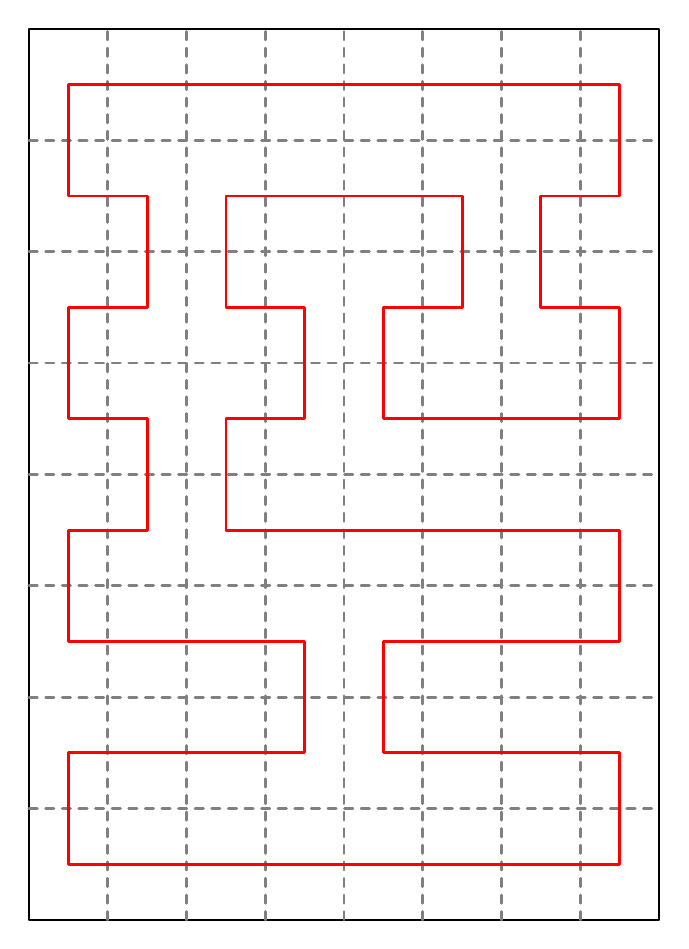
\begin{tikzpicture}[x=1.0cm,y=1.4142135623730951cm,line width=1pt,line cap=round,line join=round]
\draw (0,0) rectangle (8,8);
\draw[dashed,gray] (1,0) -- (1,8) (2,0) -- (2,8) (3,0) -- (3,8) (4,0) -- (4,8) (5,0) -- (5,8) (6,0) -- (6,8) (7,0) -- (7,8) (0,1) -- (8,1) (0,2) -- (8,2) (0,3) -- (8,3) (0,4) -- (8,4) (0,5) -- (8,5) (0,6) -- (8,6) (0,7) -- (8,7);
\draw[red] (0.5,0.5) -- (1.5,0.5) -- (2.5,0.5) -- (3.5,0.5) -- (4.5,0.5) -- (5.5,0.5) -- (6.5,0.5) -- (7.5,0.5) -- (7.5,1.5) -- (6.5,1.5) -- (5.5,1.5) -- (4.5,1.5) -- (4.5,2.5) -- (5.5,2.5) -- (6.5,2.5) -- (7.5,2.5) -- (7.5,3.5) -- (6.5,3.5) -- (5.5,3.5) -- (4.5,3.5) -- (3.5,3.5) -- (2.5,3.5) -- (2.5,4.5) -- (3.5,4.5) -- (3.5,5.5) -- (2.5,5.5) -- (2.5,6.5) -- (3.5,6.5) -- (4.5,6.5) -- (5.5,6.5) -- (5.5,5.5) -- (4.5,5.5) -- (4.5,4.5) -- (5.5,4.5) -- (6.5,4.5) -- (7.5,4.5) -- (7.5,5.5) -- (6.5,5.5) -- (6.5,6.5) -- (7.5,6.5) -- (7.5,7.5) -- (6.5,7.5) -- (5.5,7.5) -- (4.5,7.5) -- (3.5,7.5) -- (2.5,7.5) -- (1.5,7.5) -- (0.5,7.5) -- (0.5,6.5) -- (1.5,6.5) -- (1.5,5.5) -- (0.5,5.5) -- (0.5,4.5) -- (1.5,4.5) -- (1.5,3.5) -- (0.5,3.5) -- (0.5,2.5) -- (1.5,2.5) -- (2.5,2.5) -- (3.5,2.5) -- (3.5,1.5) -- (2.5,1.5) -- (1.5,1.5) -- (0.5,1.5) -- (0.5,0.5) -- cycle;\end{tikzpicture}
\hspace{5mm}
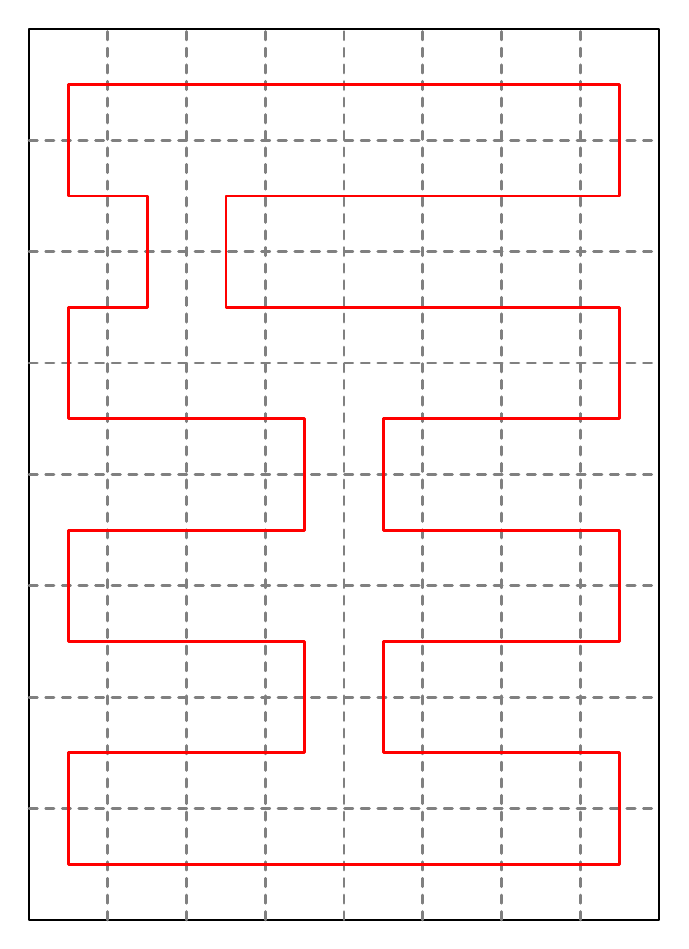
\begin{tikzpicture}[x=1.0cm,y=1.4142135623730951cm,line width=1pt,line cap=round,line join=round]
\draw (0,0) rectangle (8,8);
\draw[dashed,gray] (1,0) -- (1,8) (2,0) -- (2,8) (3,0) -- (3,8) (4,0) -- (4,8) (5,0) -- (5,8) (6,0) -- (6,8) (7,0) -- (7,8) (0,1) -- (8,1) (0,2) -- (8,2) (0,3) -- (8,3) (0,4) -- (8,4) (0,5) -- (8,5) (0,6) -- (8,6) (0,7) -- (8,7);
\draw[red] (0.5,0.5) -- (1.5,0.5) -- (2.5,0.5) -- (3.5,0.5) -- (4.5,0.5) -- (5.5,0.5) -- (6.5,0.5) -- (7.5,0.5) -- (7.5,1.5) -- (6.5,1.5) -- (5.5,1.5) -- (4.5,1.5) -- (4.5,2.5) -- (5.5,2.5) -- (6.5,2.5) -- (7.5,2.5) -- (7.5,3.5) -- (6.5,3.5) -- (5.5,3.5) -- (4.5,3.5) -- (4.5,4.5) -- (5.5,4.5) -- (6.5,4.5) -- (7.5,4.5) -- (7.5,5.5) -- (6.5,5.5) -- (5.5,5.5) -- (4.5,5.5) -- (3.5,5.5) -- (2.5,5.5) -- (2.5,6.5) -- (3.5,6.5) -- (4.5,6.5) -- (5.5,6.5) -- (6.5,6.5) -- (7.5,6.5) -- (7.5,7.5) -- (6.5,7.5) -- (5.5,7.5) -- (4.5,7.5) -- (3.5,7.5) -- (2.5,7.5) -- (1.5,7.5) -- (0.5,7.5) -- (0.5,6.5) -- (1.5,6.5) -- (1.5,5.5) -- (0.5,5.5) -- (0.5,4.5) -- (1.5,4.5) -- (2.5,4.5) -- (3.5,4.5) -- (3.5,3.5) -- (2.5,3.5) -- (1.5,3.5) -- (0.5,3.5) -- (0.5,2.5) -- (1.5,2.5) -- (2.5,2.5) -- (3.5,2.5) -- (3.5,1.5) -- (2.5,1.5) -- (1.5,1.5) -- (0.5,1.5) -- (0.5,0.5) -- cycle;\end{tikzpicture}

\vspace{5mm}

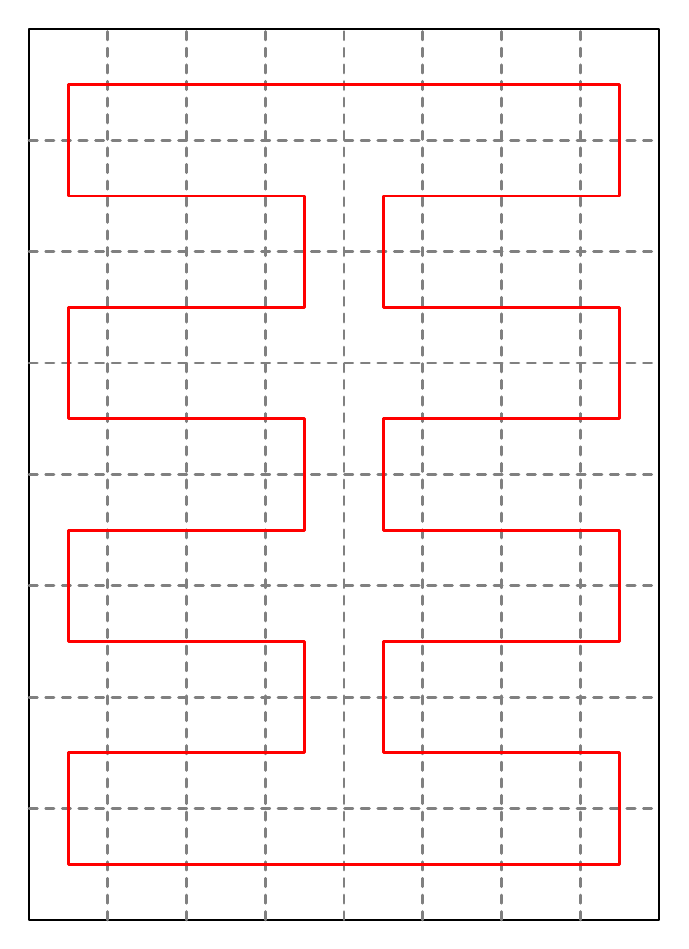
\begin{tikzpicture}[x=1.0cm,y=1.4142135623730951cm,line width=1pt,line cap=round,line join=round]
\draw (0,0) rectangle (8,8);
\draw[dashed,gray] (1,0) -- (1,8) (2,0) -- (2,8) (3,0) -- (3,8) (4,0) -- (4,8) (5,0) -- (5,8) (6,0) -- (6,8) (7,0) -- (7,8) (0,1) -- (8,1) (0,2) -- (8,2) (0,3) -- (8,3) (0,4) -- (8,4) (0,5) -- (8,5) (0,6) -- (8,6) (0,7) -- (8,7);
\draw[red] (0.5,0.5) -- (1.5,0.5) -- (2.5,0.5) -- (3.5,0.5) -- (4.5,0.5) -- (5.5,0.5) -- (6.5,0.5) -- (7.5,0.5) -- (7.5,1.5) -- (6.5,1.5) -- (5.5,1.5) -- (4.5,1.5) -- (4.5,2.5) -- (5.5,2.5) -- (6.5,2.5) -- (7.5,2.5) -- (7.5,3.5) -- (6.5,3.5) -- (5.5,3.5) -- (4.5,3.5) -- (4.5,4.5) -- (5.5,4.5) -- (6.5,4.5) -- (7.5,4.5) -- (7.5,5.5) -- (6.5,5.5) -- (5.5,5.5) -- (4.5,5.5) -- (4.5,6.5) -- (5.5,6.5) -- (6.5,6.5) -- (7.5,6.5) -- (7.5,7.5) -- (6.5,7.5) -- (5.5,7.5) -- (4.5,7.5) -- (3.5,7.5) -- (2.5,7.5) -- (1.5,7.5) -- (0.5,7.5) -- (0.5,6.5) -- (1.5,6.5) -- (2.5,6.5) -- (3.5,6.5) -- (3.5,5.5) -- (2.5,5.5) -- (1.5,5.5) -- (0.5,5.5) -- (0.5,4.5) -- (1.5,4.5) -- (2.5,4.5) -- (3.5,4.5) -- (3.5,3.5) -- (2.5,3.5) -- (1.5,3.5) -- (0.5,3.5) -- (0.5,2.5) -- (1.5,2.5) -- (2.5,2.5) -- (3.5,2.5) -- (3.5,1.5) -- (2.5,1.5) -- (1.5,1.5) -- (0.5,1.5) -- (0.5,0.5) -- cycle;\end{tikzpicture}
\hspace{5mm}
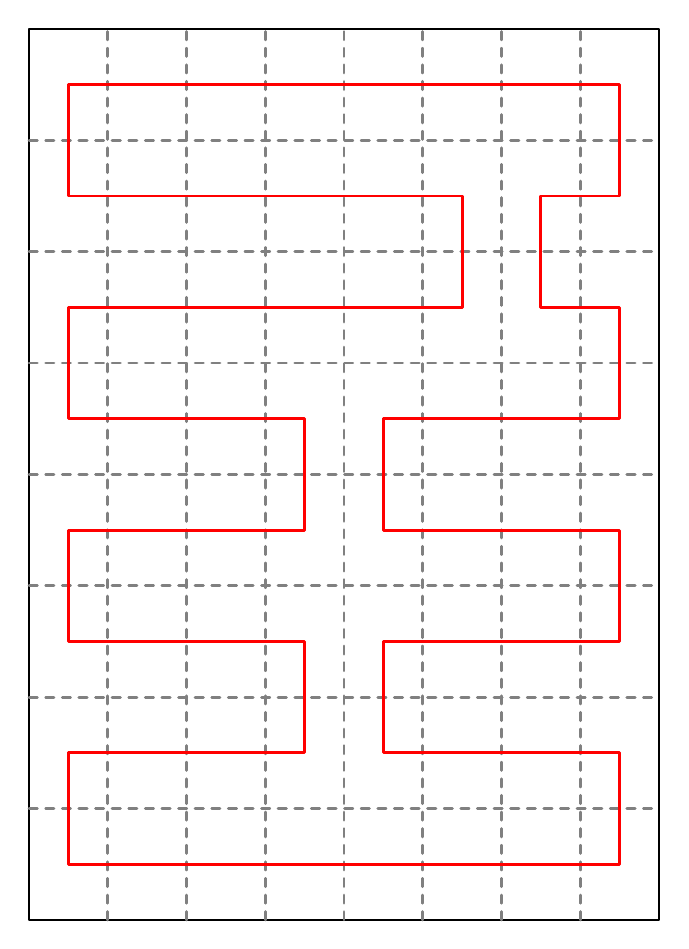
\begin{tikzpicture}[x=1.0cm,y=1.4142135623730951cm,line width=1pt,line cap=round,line join=round]
\draw (0,0) rectangle (8,8);
\draw[dashed,gray] (1,0) -- (1,8) (2,0) -- (2,8) (3,0) -- (3,8) (4,0) -- (4,8) (5,0) -- (5,8) (6,0) -- (6,8) (7,0) -- (7,8) (0,1) -- (8,1) (0,2) -- (8,2) (0,3) -- (8,3) (0,4) -- (8,4) (0,5) -- (8,5) (0,6) -- (8,6) (0,7) -- (8,7);
\draw[red] (0.5,0.5) -- (1.5,0.5) -- (2.5,0.5) -- (3.5,0.5) -- (4.5,0.5) -- (5.5,0.5) -- (6.5,0.5) -- (7.5,0.5) -- (7.5,1.5) -- (6.5,1.5) -- (5.5,1.5) -- (4.5,1.5) -- (4.5,2.5) -- (5.5,2.5) -- (6.5,2.5) -- (7.5,2.5) -- (7.5,3.5) -- (6.5,3.5) -- (5.5,3.5) -- (4.5,3.5) -- (4.5,4.5) -- (5.5,4.5) -- (6.5,4.5) -- (7.5,4.5) -- (7.5,5.5) -- (6.5,5.5) -- (6.5,6.5) -- (7.5,6.5) -- (7.5,7.5) -- (6.5,7.5) -- (5.5,7.5) -- (4.5,7.5) -- (3.5,7.5) -- (2.5,7.5) -- (1.5,7.5) -- (0.5,7.5) -- (0.5,6.5) -- (1.5,6.5) -- (2.5,6.5) -- (3.5,6.5) -- (4.5,6.5) -- (5.5,6.5) -- (5.5,5.5) -- (4.5,5.5) -- (3.5,5.5) -- (2.5,5.5) -- (1.5,5.5) -- (0.5,5.5) -- (0.5,4.5) -- (1.5,4.5) -- (2.5,4.5) -- (3.5,4.5) -- (3.5,3.5) -- (2.5,3.5) -- (1.5,3.5) -- (0.5,3.5) -- (0.5,2.5) -- (1.5,2.5) -- (2.5,2.5) -- (3.5,2.5) -- (3.5,1.5) -- (2.5,1.5) -- (1.5,1.5) -- (0.5,1.5) -- (0.5,0.5) -- cycle;\end{tikzpicture}

\vspace{5mm}

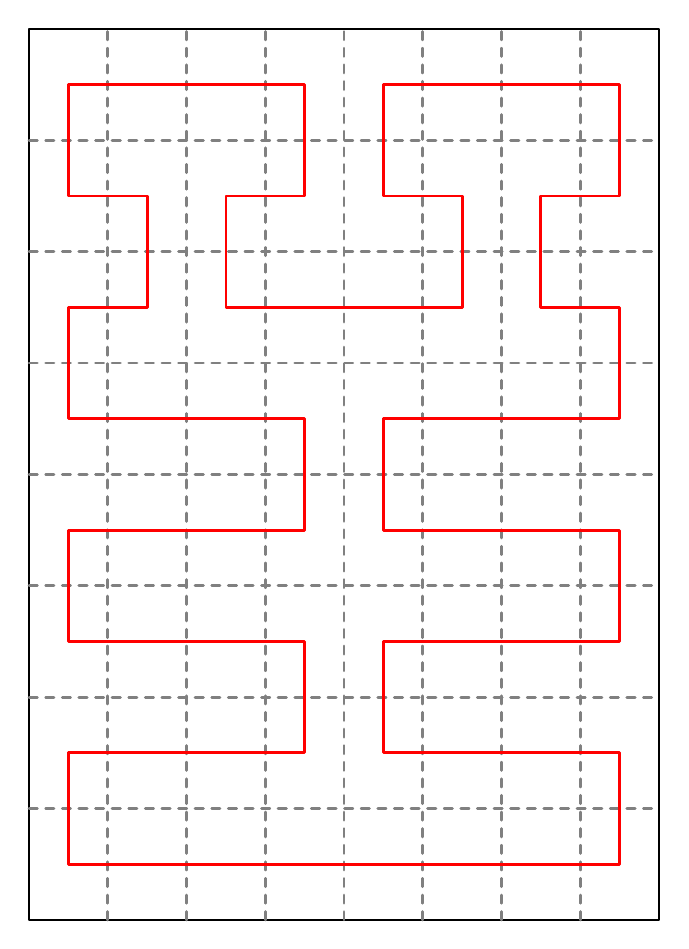
\begin{tikzpicture}[x=1.0cm,y=1.4142135623730951cm,line width=1pt,line cap=round,line join=round]
\draw (0,0) rectangle (8,8);
\draw[dashed,gray] (1,0) -- (1,8) (2,0) -- (2,8) (3,0) -- (3,8) (4,0) -- (4,8) (5,0) -- (5,8) (6,0) -- (6,8) (7,0) -- (7,8) (0,1) -- (8,1) (0,2) -- (8,2) (0,3) -- (8,3) (0,4) -- (8,4) (0,5) -- (8,5) (0,6) -- (8,6) (0,7) -- (8,7);
\draw[red] (0.5,0.5) -- (1.5,0.5) -- (2.5,0.5) -- (3.5,0.5) -- (4.5,0.5) -- (5.5,0.5) -- (6.5,0.5) -- (7.5,0.5) -- (7.5,1.5) -- (6.5,1.5) -- (5.5,1.5) -- (4.5,1.5) -- (4.5,2.5) -- (5.5,2.5) -- (6.5,2.5) -- (7.5,2.5) -- (7.5,3.5) -- (6.5,3.5) -- (5.5,3.5) -- (4.5,3.5) -- (4.5,4.5) -- (5.5,4.5) -- (6.5,4.5) -- (7.5,4.5) -- (7.5,5.5) -- (6.5,5.5) -- (6.5,6.5) -- (7.5,6.5) -- (7.5,7.5) -- (6.5,7.5) -- (5.5,7.5) -- (4.5,7.5) -- (4.5,6.5) -- (5.5,6.5) -- (5.5,5.5) -- (4.5,5.5) -- (3.5,5.5) -- (2.5,5.5) -- (2.5,6.5) -- (3.5,6.5) -- (3.5,7.5) -- (2.5,7.5) -- (1.5,7.5) -- (0.5,7.5) -- (0.5,6.5) -- (1.5,6.5) -- (1.5,5.5) -- (0.5,5.5) -- (0.5,4.5) -- (1.5,4.5) -- (2.5,4.5) -- (3.5,4.5) -- (3.5,3.5) -- (2.5,3.5) -- (1.5,3.5) -- (0.5,3.5) -- (0.5,2.5) -- (1.5,2.5) -- (2.5,2.5) -- (3.5,2.5) -- (3.5,1.5) -- (2.5,1.5) -- (1.5,1.5) -- (0.5,1.5) -- (0.5,0.5) -- cycle;\end{tikzpicture}
\hspace{5mm}
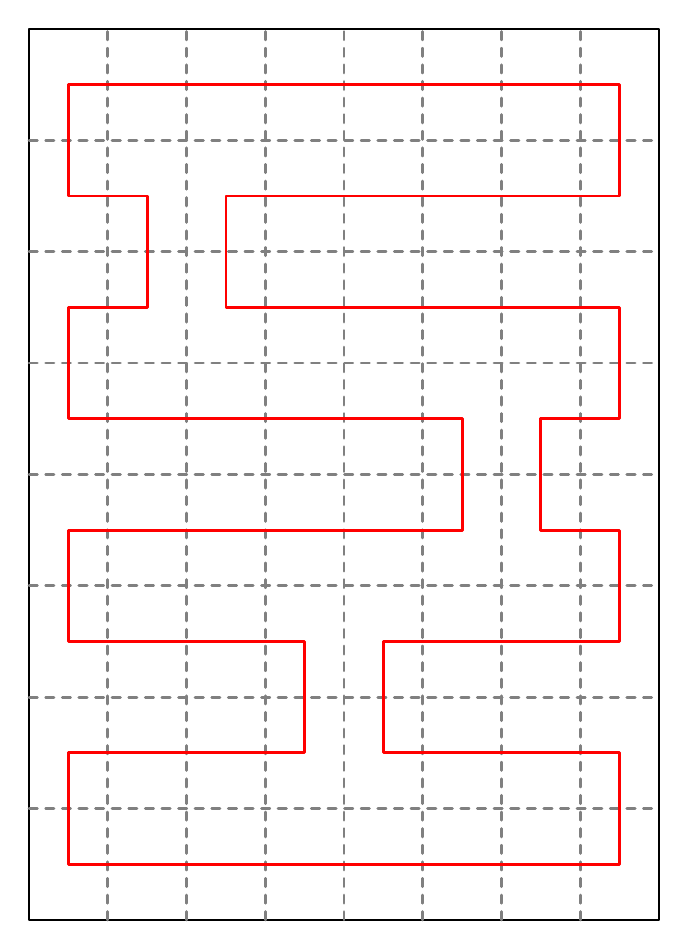
\begin{tikzpicture}[x=1.0cm,y=1.4142135623730951cm,line width=1pt,line cap=round,line join=round]
\draw (0,0) rectangle (8,8);
\draw[dashed,gray] (1,0) -- (1,8) (2,0) -- (2,8) (3,0) -- (3,8) (4,0) -- (4,8) (5,0) -- (5,8) (6,0) -- (6,8) (7,0) -- (7,8) (0,1) -- (8,1) (0,2) -- (8,2) (0,3) -- (8,3) (0,4) -- (8,4) (0,5) -- (8,5) (0,6) -- (8,6) (0,7) -- (8,7);
\draw[red] (0.5,0.5) -- (1.5,0.5) -- (2.5,0.5) -- (3.5,0.5) -- (4.5,0.5) -- (5.5,0.5) -- (6.5,0.5) -- (7.5,0.5) -- (7.5,1.5) -- (6.5,1.5) -- (5.5,1.5) -- (4.5,1.5) -- (4.5,2.5) -- (5.5,2.5) -- (6.5,2.5) -- (7.5,2.5) -- (7.5,3.5) -- (6.5,3.5) -- (6.5,4.5) -- (7.5,4.5) -- (7.5,5.5) -- (6.5,5.5) -- (5.5,5.5) -- (4.5,5.5) -- (3.5,5.5) -- (2.5,5.5) -- (2.5,6.5) -- (3.5,6.5) -- (4.5,6.5) -- (5.5,6.5) -- (6.5,6.5) -- (7.5,6.5) -- (7.5,7.5) -- (6.5,7.5) -- (5.5,7.5) -- (4.5,7.5) -- (3.5,7.5) -- (2.5,7.5) -- (1.5,7.5) -- (0.5,7.5) -- (0.5,6.5) -- (1.5,6.5) -- (1.5,5.5) -- (0.5,5.5) -- (0.5,4.5) -- (1.5,4.5) -- (2.5,4.5) -- (3.5,4.5) -- (4.5,4.5) -- (5.5,4.5) -- (5.5,3.5) -- (4.5,3.5) -- (3.5,3.5) -- (2.5,3.5) -- (1.5,3.5) -- (0.5,3.5) -- (0.5,2.5) -- (1.5,2.5) -- (2.5,2.5) -- (3.5,2.5) -- (3.5,1.5) -- (2.5,1.5) -- (1.5,1.5) -- (0.5,1.5) -- (0.5,0.5) -- cycle;\end{tikzpicture}

\vspace{5mm}

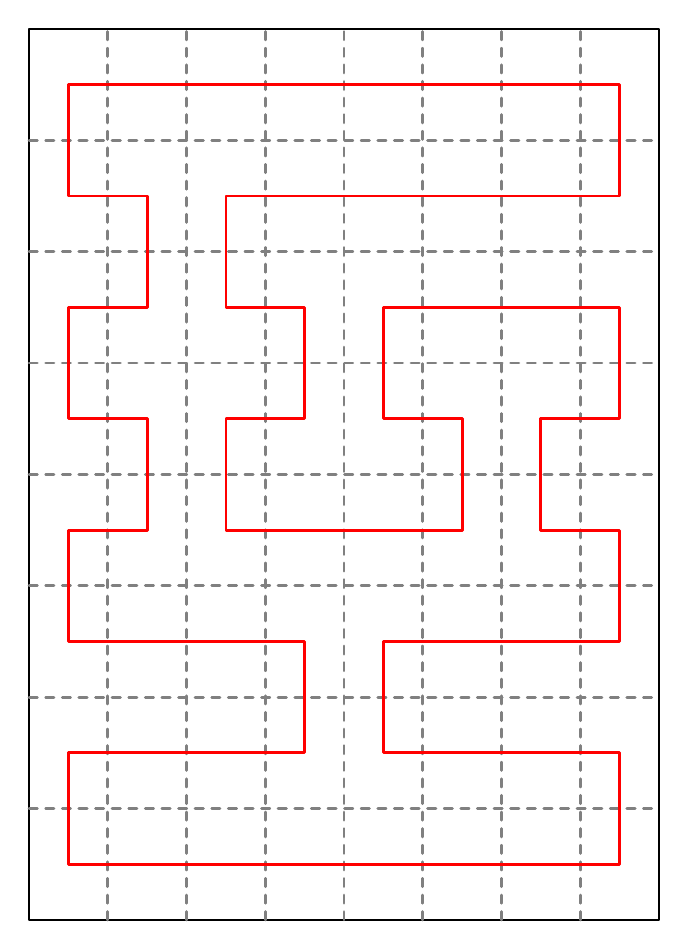
\begin{tikzpicture}[x=1.0cm,y=1.4142135623730951cm,line width=1pt,line cap=round,line join=round]
\draw (0,0) rectangle (8,8);
\draw[dashed,gray] (1,0) -- (1,8) (2,0) -- (2,8) (3,0) -- (3,8) (4,0) -- (4,8) (5,0) -- (5,8) (6,0) -- (6,8) (7,0) -- (7,8) (0,1) -- (8,1) (0,2) -- (8,2) (0,3) -- (8,3) (0,4) -- (8,4) (0,5) -- (8,5) (0,6) -- (8,6) (0,7) -- (8,7);
\draw[red] (0.5,0.5) -- (1.5,0.5) -- (2.5,0.5) -- (3.5,0.5) -- (4.5,0.5) -- (5.5,0.5) -- (6.5,0.5) -- (7.5,0.5) -- (7.5,1.5) -- (6.5,1.5) -- (5.5,1.5) -- (4.5,1.5) -- (4.5,2.5) -- (5.5,2.5) -- (6.5,2.5) -- (7.5,2.5) -- (7.5,3.5) -- (6.5,3.5) -- (6.5,4.5) -- (7.5,4.5) -- (7.5,5.5) -- (6.5,5.5) -- (5.5,5.5) -- (4.5,5.5) -- (4.5,4.5) -- (5.5,4.5) -- (5.5,3.5) -- (4.5,3.5) -- (3.5,3.5) -- (2.5,3.5) -- (2.5,4.5) -- (3.5,4.5) -- (3.5,5.5) -- (2.5,5.5) -- (2.5,6.5) -- (3.5,6.5) -- (4.5,6.5) -- (5.5,6.5) -- (6.5,6.5) -- (7.5,6.5) -- (7.5,7.5) -- (6.5,7.5) -- (5.5,7.5) -- (4.5,7.5) -- (3.5,7.5) -- (2.5,7.5) -- (1.5,7.5) -- (0.5,7.5) -- (0.5,6.5) -- (1.5,6.5) -- (1.5,5.5) -- (0.5,5.5) -- (0.5,4.5) -- (1.5,4.5) -- (1.5,3.5) -- (0.5,3.5) -- (0.5,2.5) -- (1.5,2.5) -- (2.5,2.5) -- (3.5,2.5) -- (3.5,1.5) -- (2.5,1.5) -- (1.5,1.5) -- (0.5,1.5) -- (0.5,0.5) -- cycle;\end{tikzpicture}
\hspace{5mm}
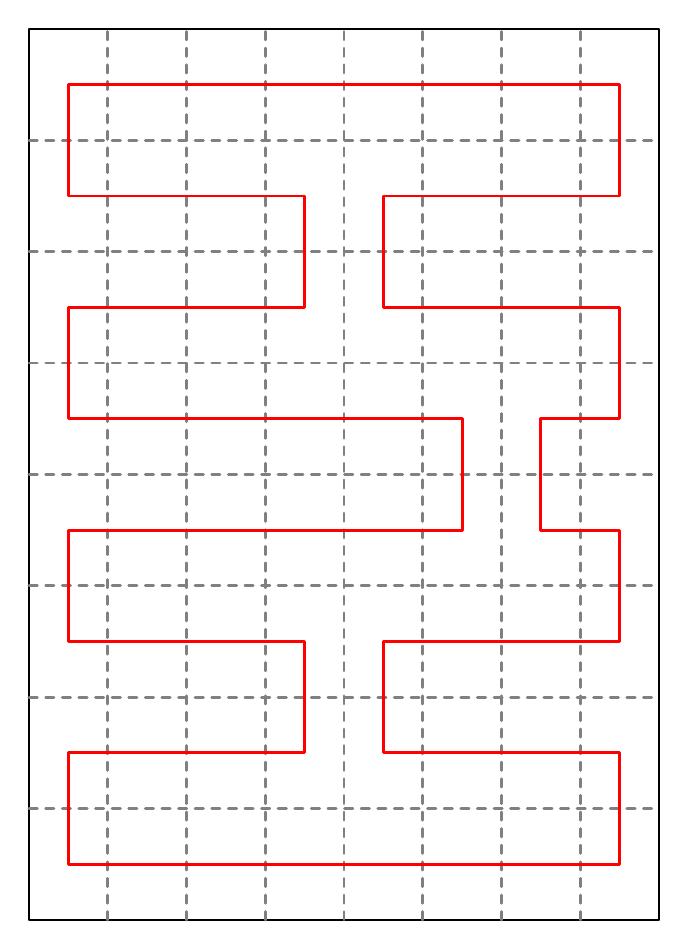
\begin{tikzpicture}[x=1.0cm,y=1.4142135623730951cm,line width=1pt,line cap=round,line join=round]
\draw (0,0) rectangle (8,8);
\draw[dashed,gray] (1,0) -- (1,8) (2,0) -- (2,8) (3,0) -- (3,8) (4,0) -- (4,8) (5,0) -- (5,8) (6,0) -- (6,8) (7,0) -- (7,8) (0,1) -- (8,1) (0,2) -- (8,2) (0,3) -- (8,3) (0,4) -- (8,4) (0,5) -- (8,5) (0,6) -- (8,6) (0,7) -- (8,7);
\draw[red] (0.5,0.5) -- (1.5,0.5) -- (2.5,0.5) -- (3.5,0.5) -- (4.5,0.5) -- (5.5,0.5) -- (6.5,0.5) -- (7.5,0.5) -- (7.5,1.5) -- (6.5,1.5) -- (5.5,1.5) -- (4.5,1.5) -- (4.5,2.5) -- (5.5,2.5) -- (6.5,2.5) -- (7.5,2.5) -- (7.5,3.5) -- (6.5,3.5) -- (6.5,4.5) -- (7.5,4.5) -- (7.5,5.5) -- (6.5,5.5) -- (5.5,5.5) -- (4.5,5.5) -- (4.5,6.5) -- (5.5,6.5) -- (6.5,6.5) -- (7.5,6.5) -- (7.5,7.5) -- (6.5,7.5) -- (5.5,7.5) -- (4.5,7.5) -- (3.5,7.5) -- (2.5,7.5) -- (1.5,7.5) -- (0.5,7.5) -- (0.5,6.5) -- (1.5,6.5) -- (2.5,6.5) -- (3.5,6.5) -- (3.5,5.5) -- (2.5,5.5) -- (1.5,5.5) -- (0.5,5.5) -- (0.5,4.5) -- (1.5,4.5) -- (2.5,4.5) -- (3.5,4.5) -- (4.5,4.5) -- (5.5,4.5) -- (5.5,3.5) -- (4.5,3.5) -- (3.5,3.5) -- (2.5,3.5) -- (1.5,3.5) -- (0.5,3.5) -- (0.5,2.5) -- (1.5,2.5) -- (2.5,2.5) -- (3.5,2.5) -- (3.5,1.5) -- (2.5,1.5) -- (1.5,1.5) -- (0.5,1.5) -- (0.5,0.5) -- cycle;\end{tikzpicture}

\vspace{5mm}

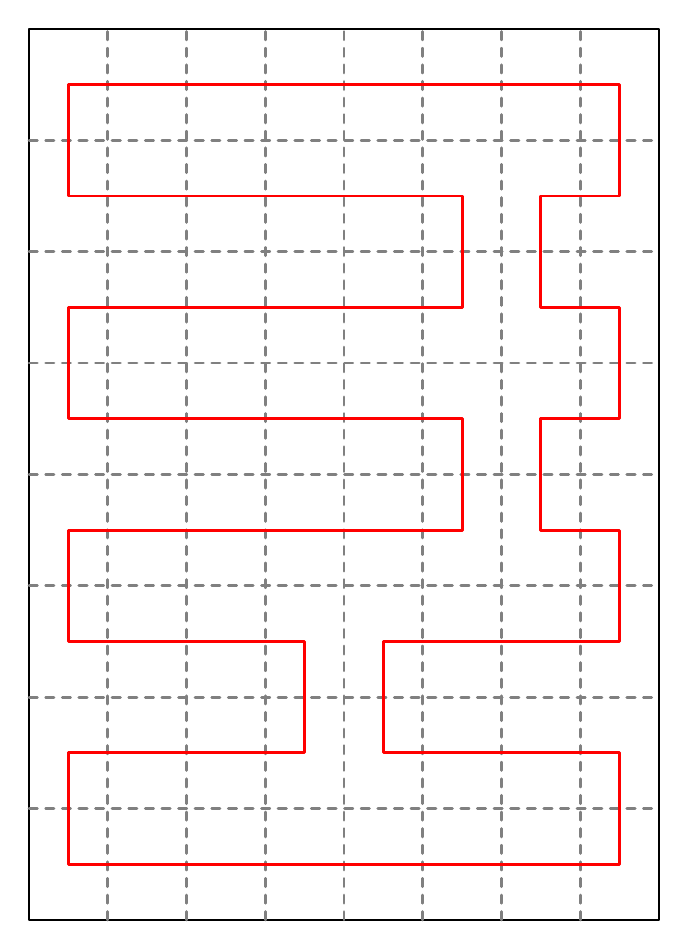
\begin{tikzpicture}[x=1.0cm,y=1.4142135623730951cm,line width=1pt,line cap=round,line join=round]
\draw (0,0) rectangle (8,8);
\draw[dashed,gray] (1,0) -- (1,8) (2,0) -- (2,8) (3,0) -- (3,8) (4,0) -- (4,8) (5,0) -- (5,8) (6,0) -- (6,8) (7,0) -- (7,8) (0,1) -- (8,1) (0,2) -- (8,2) (0,3) -- (8,3) (0,4) -- (8,4) (0,5) -- (8,5) (0,6) -- (8,6) (0,7) -- (8,7);
\draw[red] (0.5,0.5) -- (1.5,0.5) -- (2.5,0.5) -- (3.5,0.5) -- (4.5,0.5) -- (5.5,0.5) -- (6.5,0.5) -- (7.5,0.5) -- (7.5,1.5) -- (6.5,1.5) -- (5.5,1.5) -- (4.5,1.5) -- (4.5,2.5) -- (5.5,2.5) -- (6.5,2.5) -- (7.5,2.5) -- (7.5,3.5) -- (6.5,3.5) -- (6.5,4.5) -- (7.5,4.5) -- (7.5,5.5) -- (6.5,5.5) -- (6.5,6.5) -- (7.5,6.5) -- (7.5,7.5) -- (6.5,7.5) -- (5.5,7.5) -- (4.5,7.5) -- (3.5,7.5) -- (2.5,7.5) -- (1.5,7.5) -- (0.5,7.5) -- (0.5,6.5) -- (1.5,6.5) -- (2.5,6.5) -- (3.5,6.5) -- (4.5,6.5) -- (5.5,6.5) -- (5.5,5.5) -- (4.5,5.5) -- (3.5,5.5) -- (2.5,5.5) -- (1.5,5.5) -- (0.5,5.5) -- (0.5,4.5) -- (1.5,4.5) -- (2.5,4.5) -- (3.5,4.5) -- (4.5,4.5) -- (5.5,4.5) -- (5.5,3.5) -- (4.5,3.5) -- (3.5,3.5) -- (2.5,3.5) -- (1.5,3.5) -- (0.5,3.5) -- (0.5,2.5) -- (1.5,2.5) -- (2.5,2.5) -- (3.5,2.5) -- (3.5,1.5) -- (2.5,1.5) -- (1.5,1.5) -- (0.5,1.5) -- (0.5,0.5) -- cycle;\end{tikzpicture}
\hspace{5mm}
\begin{tikzpicture}[x=1.0cm,y=1.4142135623730951cm,line width=1pt,line cap=round,line join=round]
\draw (0,0) rectangle (8,8);
\draw[dashed,gray] (1,0) -- (1,8) (2,0) -- (2,8) (3,0) -- (3,8) (4,0) -- (4,8) (5,0) -- (5,8) (6,0) -- (6,8) (7,0) -- (7,8) (0,1) -- (8,1) (0,2) -- (8,2) (0,3) -- (8,3) (0,4) -- (8,4) (0,5) -- (8,5) (0,6) -- (8,6) (0,7) -- (8,7);
\draw[red] (0.5,0.5) -- (1.5,0.5) -- (2.5,0.5) -- (3.5,0.5) -- (4.5,0.5) -- (5.5,0.5) -- (6.5,0.5) -- (7.5,0.5) -- (7.5,1.5) -- (6.5,1.5) -- (5.5,1.5) -- (4.5,1.5) -- (4.5,2.5) -- (5.5,2.5) -- (6.5,2.5) -- (7.5,2.5) -- (7.5,3.5) -- (6.5,3.5) -- (6.5,4.5) -- (7.5,4.5) -- (7.5,5.5) -- (6.5,5.5) -- (6.5,6.5) -- (7.5,6.5) -- (7.5,7.5) -- (6.5,7.5) -- (5.5,7.5) -- (4.5,7.5) -- (3.5,7.5) -- (2.5,7.5) -- (1.5,7.5) -- (0.5,7.5) -- (0.5,6.5) -- (1.5,6.5) -- (2.5,6.5) -- (3.5,6.5) -- (4.5,6.5) -- (5.5,6.5) -- (5.5,5.5) -- (4.5,5.5) -- (4.5,4.5) -- (5.5,4.5) -- (5.5,3.5) -- (4.5,3.5) -- (3.5,3.5) -- (2.5,3.5) -- (2.5,4.5) -- (3.5,4.5) -- (3.5,5.5) -- (2.5,5.5) -- (1.5,5.5) -- (0.5,5.5) -- (0.5,4.5) -- (1.5,4.5) -- (1.5,3.5) -- (0.5,3.5) -- (0.5,2.5) -- (1.5,2.5) -- (2.5,2.5) -- (3.5,2.5) -- (3.5,1.5) -- (2.5,1.5) -- (1.5,1.5) -- (0.5,1.5) -- (0.5,0.5) -- cycle;\end{tikzpicture}

\vspace{5mm}

\begin{tikzpicture}[x=1.0cm,y=1.4142135623730951cm,line width=1pt,line cap=round,line join=round]
\draw (0,0) rectangle (8,8);
\draw[dashed,gray] (1,0) -- (1,8) (2,0) -- (2,8) (3,0) -- (3,8) (4,0) -- (4,8) (5,0) -- (5,8) (6,0) -- (6,8) (7,0) -- (7,8) (0,1) -- (8,1) (0,2) -- (8,2) (0,3) -- (8,3) (0,4) -- (8,4) (0,5) -- (8,5) (0,6) -- (8,6) (0,7) -- (8,7);
\draw[red] (0.5,0.5) -- (1.5,0.5) -- (2.5,0.5) -- (3.5,0.5) -- (4.5,0.5) -- (5.5,0.5) -- (6.5,0.5) -- (7.5,0.5) -- (7.5,1.5) -- (6.5,1.5) -- (5.5,1.5) -- (4.5,1.5) -- (4.5,2.5) -- (5.5,2.5) -- (6.5,2.5) -- (7.5,2.5) -- (7.5,3.5) -- (6.5,3.5) -- (6.5,4.5) -- (7.5,4.5) -- (7.5,5.5) -- (6.5,5.5) -- (6.5,6.5) -- (7.5,6.5) -- (7.5,7.5) -- (6.5,7.5) -- (5.5,7.5) -- (4.5,7.5) -- (3.5,7.5) -- (2.5,7.5) -- (1.5,7.5) -- (0.5,7.5) -- (0.5,6.5) -- (1.5,6.5) -- (1.5,5.5) -- (0.5,5.5) -- (0.5,4.5) -- (1.5,4.5) -- (2.5,4.5) -- (3.5,4.5) -- (3.5,5.5) -- (2.5,5.5) -- (2.5,6.5) -- (3.5,6.5) -- (4.5,6.5) -- (5.5,6.5) -- (5.5,5.5) -- (4.5,5.5) -- (4.5,4.5) -- (5.5,4.5) -- (5.5,3.5) -- (4.5,3.5) -- (3.5,3.5) -- (2.5,3.5) -- (1.5,3.5) -- (0.5,3.5) -- (0.5,2.5) -- (1.5,2.5) -- (2.5,2.5) -- (3.5,2.5) -- (3.5,1.5) -- (2.5,1.5) -- (1.5,1.5) -- (0.5,1.5) -- (0.5,0.5) -- cycle;\end{tikzpicture}
\hspace{5mm}
\begin{tikzpicture}[x=1.0cm,y=1.4142135623730951cm,line width=1pt,line cap=round,line join=round]
\draw (0,0) rectangle (8,8);
\draw[dashed,gray] (1,0) -- (1,8) (2,0) -- (2,8) (3,0) -- (3,8) (4,0) -- (4,8) (5,0) -- (5,8) (6,0) -- (6,8) (7,0) -- (7,8) (0,1) -- (8,1) (0,2) -- (8,2) (0,3) -- (8,3) (0,4) -- (8,4) (0,5) -- (8,5) (0,6) -- (8,6) (0,7) -- (8,7);
\draw[red] (0.5,0.5) -- (1.5,0.5) -- (2.5,0.5) -- (3.5,0.5) -- (4.5,0.5) -- (5.5,0.5) -- (6.5,0.5) -- (7.5,0.5) -- (7.5,1.5) -- (6.5,1.5) -- (5.5,1.5) -- (4.5,1.5) -- (4.5,2.5) -- (5.5,2.5) -- (6.5,2.5) -- (7.5,2.5) -- (7.5,3.5) -- (6.5,3.5) -- (6.5,4.5) -- (7.5,4.5) -- (7.5,5.5) -- (6.5,5.5) -- (6.5,6.5) -- (7.5,6.5) -- (7.5,7.5) -- (6.5,7.5) -- (5.5,7.5) -- (4.5,7.5) -- (4.5,6.5) -- (5.5,6.5) -- (5.5,5.5) -- (4.5,5.5) -- (3.5,5.5) -- (2.5,5.5) -- (2.5,6.5) -- (3.5,6.5) -- (3.5,7.5) -- (2.5,7.5) -- (1.5,7.5) -- (0.5,7.5) -- (0.5,6.5) -- (1.5,6.5) -- (1.5,5.5) -- (0.5,5.5) -- (0.5,4.5) -- (1.5,4.5) -- (2.5,4.5) -- (3.5,4.5) -- (4.5,4.5) -- (5.5,4.5) -- (5.5,3.5) -- (4.5,3.5) -- (3.5,3.5) -- (2.5,3.5) -- (1.5,3.5) -- (0.5,3.5) -- (0.5,2.5) -- (1.5,2.5) -- (2.5,2.5) -- (3.5,2.5) -- (3.5,1.5) -- (2.5,1.5) -- (1.5,1.5) -- (0.5,1.5) -- (0.5,0.5) -- cycle;\end{tikzpicture}

\vspace{5mm}

\begin{tikzpicture}[x=1.0cm,y=1.4142135623730951cm,line width=1pt,line cap=round,line join=round]
\draw (0,0) rectangle (8,8);
\draw[dashed,gray] (1,0) -- (1,8) (2,0) -- (2,8) (3,0) -- (3,8) (4,0) -- (4,8) (5,0) -- (5,8) (6,0) -- (6,8) (7,0) -- (7,8) (0,1) -- (8,1) (0,2) -- (8,2) (0,3) -- (8,3) (0,4) -- (8,4) (0,5) -- (8,5) (0,6) -- (8,6) (0,7) -- (8,7);
\draw[red] (0.5,0.5) -- (1.5,0.5) -- (2.5,0.5) -- (3.5,0.5) -- (4.5,0.5) -- (5.5,0.5) -- (6.5,0.5) -- (7.5,0.5) -- (7.5,1.5) -- (6.5,1.5) -- (5.5,1.5) -- (4.5,1.5) -- (4.5,2.5) -- (5.5,2.5) -- (6.5,2.5) -- (7.5,2.5) -- (7.5,3.5) -- (6.5,3.5) -- (6.5,4.5) -- (7.5,4.5) -- (7.5,5.5) -- (6.5,5.5) -- (6.5,6.5) -- (7.5,6.5) -- (7.5,7.5) -- (6.5,7.5) -- (5.5,7.5) -- (4.5,7.5) -- (4.5,6.5) -- (5.5,6.5) -- (5.5,5.5) -- (4.5,5.5) -- (4.5,4.5) -- (5.5,4.5) -- (5.5,3.5) -- (4.5,3.5) -- (3.5,3.5) -- (2.5,3.5) -- (2.5,4.5) -- (3.5,4.5) -- (3.5,5.5) -- (2.5,5.5) -- (2.5,6.5) -- (3.5,6.5) -- (3.5,7.5) -- (2.5,7.5) -- (1.5,7.5) -- (0.5,7.5) -- (0.5,6.5) -- (1.5,6.5) -- (1.5,5.5) -- (0.5,5.5) -- (0.5,4.5) -- (1.5,4.5) -- (1.5,3.5) -- (0.5,3.5) -- (0.5,2.5) -- (1.5,2.5) -- (2.5,2.5) -- (3.5,2.5) -- (3.5,1.5) -- (2.5,1.5) -- (1.5,1.5) -- (0.5,1.5) -- (0.5,0.5) -- cycle;\end{tikzpicture}
\hspace{5mm}
\begin{tikzpicture}[x=1.0cm,y=1.4142135623730951cm,line width=1pt,line cap=round,line join=round]
\draw (0,0) rectangle (8,8);
\draw[dashed,gray] (1,0) -- (1,8) (2,0) -- (2,8) (3,0) -- (3,8) (4,0) -- (4,8) (5,0) -- (5,8) (6,0) -- (6,8) (7,0) -- (7,8) (0,1) -- (8,1) (0,2) -- (8,2) (0,3) -- (8,3) (0,4) -- (8,4) (0,5) -- (8,5) (0,6) -- (8,6) (0,7) -- (8,7);
\draw[red] (0.5,0.5) -- (1.5,0.5) -- (2.5,0.5) -- (3.5,0.5) -- (4.5,0.5) -- (5.5,0.5) -- (6.5,0.5) -- (7.5,0.5) -- (7.5,1.5) -- (6.5,1.5) -- (6.5,2.5) -- (7.5,2.5) -- (7.5,3.5) -- (6.5,3.5) -- (5.5,3.5) -- (4.5,3.5) -- (3.5,3.5) -- (2.5,3.5) -- (2.5,4.5) -- (3.5,4.5) -- (4.5,4.5) -- (5.5,4.5) -- (6.5,4.5) -- (7.5,4.5) -- (7.5,5.5) -- (6.5,5.5) -- (5.5,5.5) -- (4.5,5.5) -- (3.5,5.5) -- (2.5,5.5) -- (2.5,6.5) -- (3.5,6.5) -- (4.5,6.5) -- (5.5,6.5) -- (6.5,6.5) -- (7.5,6.5) -- (7.5,7.5) -- (6.5,7.5) -- (5.5,7.5) -- (4.5,7.5) -- (3.5,7.5) -- (2.5,7.5) -- (1.5,7.5) -- (0.5,7.5) -- (0.5,6.5) -- (1.5,6.5) -- (1.5,5.5) -- (0.5,5.5) -- (0.5,4.5) -- (1.5,4.5) -- (1.5,3.5) -- (0.5,3.5) -- (0.5,2.5) -- (1.5,2.5) -- (2.5,2.5) -- (3.5,2.5) -- (4.5,2.5) -- (5.5,2.5) -- (5.5,1.5) -- (4.5,1.5) -- (3.5,1.5) -- (2.5,1.5) -- (1.5,1.5) -- (0.5,1.5) -- (0.5,0.5) -- cycle;\end{tikzpicture}

\vspace{5mm}

\begin{tikzpicture}[x=1.0cm,y=1.4142135623730951cm,line width=1pt,line cap=round,line join=round]
\draw (0,0) rectangle (8,8);
\draw[dashed,gray] (1,0) -- (1,8) (2,0) -- (2,8) (3,0) -- (3,8) (4,0) -- (4,8) (5,0) -- (5,8) (6,0) -- (6,8) (7,0) -- (7,8) (0,1) -- (8,1) (0,2) -- (8,2) (0,3) -- (8,3) (0,4) -- (8,4) (0,5) -- (8,5) (0,6) -- (8,6) (0,7) -- (8,7);
\draw[red] (0.5,0.5) -- (1.5,0.5) -- (2.5,0.5) -- (3.5,0.5) -- (4.5,0.5) -- (5.5,0.5) -- (6.5,0.5) -- (7.5,0.5) -- (7.5,1.5) -- (6.5,1.5) -- (6.5,2.5) -- (7.5,2.5) -- (7.5,3.5) -- (6.5,3.5) -- (5.5,3.5) -- (4.5,3.5) -- (3.5,3.5) -- (2.5,3.5) -- (2.5,4.5) -- (3.5,4.5) -- (4.5,4.5) -- (5.5,4.5) -- (6.5,4.5) -- (7.5,4.5) -- (7.5,5.5) -- (6.5,5.5) -- (5.5,5.5) -- (4.5,5.5) -- (4.5,6.5) -- (5.5,6.5) -- (6.5,6.5) -- (7.5,6.5) -- (7.5,7.5) -- (6.5,7.5) -- (5.5,7.5) -- (4.5,7.5) -- (3.5,7.5) -- (2.5,7.5) -- (1.5,7.5) -- (0.5,7.5) -- (0.5,6.5) -- (1.5,6.5) -- (2.5,6.5) -- (3.5,6.5) -- (3.5,5.5) -- (2.5,5.5) -- (1.5,5.5) -- (0.5,5.5) -- (0.5,4.5) -- (1.5,4.5) -- (1.5,3.5) -- (0.5,3.5) -- (0.5,2.5) -- (1.5,2.5) -- (2.5,2.5) -- (3.5,2.5) -- (4.5,2.5) -- (5.5,2.5) -- (5.5,1.5) -- (4.5,1.5) -- (3.5,1.5) -- (2.5,1.5) -- (1.5,1.5) -- (0.5,1.5) -- (0.5,0.5) -- cycle;\end{tikzpicture}
\hspace{5mm}
\begin{tikzpicture}[x=1.0cm,y=1.4142135623730951cm,line width=1pt,line cap=round,line join=round]
\draw (0,0) rectangle (8,8);
\draw[dashed,gray] (1,0) -- (1,8) (2,0) -- (2,8) (3,0) -- (3,8) (4,0) -- (4,8) (5,0) -- (5,8) (6,0) -- (6,8) (7,0) -- (7,8) (0,1) -- (8,1) (0,2) -- (8,2) (0,3) -- (8,3) (0,4) -- (8,4) (0,5) -- (8,5) (0,6) -- (8,6) (0,7) -- (8,7);
\draw[red] (0.5,0.5) -- (1.5,0.5) -- (2.5,0.5) -- (3.5,0.5) -- (4.5,0.5) -- (5.5,0.5) -- (6.5,0.5) -- (7.5,0.5) -- (7.5,1.5) -- (6.5,1.5) -- (6.5,2.5) -- (7.5,2.5) -- (7.5,3.5) -- (6.5,3.5) -- (5.5,3.5) -- (4.5,3.5) -- (3.5,3.5) -- (2.5,3.5) -- (2.5,4.5) -- (3.5,4.5) -- (4.5,4.5) -- (5.5,4.5) -- (6.5,4.5) -- (7.5,4.5) -- (7.5,5.5) -- (6.5,5.5) -- (6.5,6.5) -- (7.5,6.5) -- (7.5,7.5) -- (6.5,7.5) -- (5.5,7.5) -- (4.5,7.5) -- (3.5,7.5) -- (2.5,7.5) -- (1.5,7.5) -- (0.5,7.5) -- (0.5,6.5) -- (1.5,6.5) -- (2.5,6.5) -- (3.5,6.5) -- (4.5,6.5) -- (5.5,6.5) -- (5.5,5.5) -- (4.5,5.5) -- (3.5,5.5) -- (2.5,5.5) -- (1.5,5.5) -- (0.5,5.5) -- (0.5,4.5) -- (1.5,4.5) -- (1.5,3.5) -- (0.5,3.5) -- (0.5,2.5) -- (1.5,2.5) -- (2.5,2.5) -- (3.5,2.5) -- (4.5,2.5) -- (5.5,2.5) -- (5.5,1.5) -- (4.5,1.5) -- (3.5,1.5) -- (2.5,1.5) -- (1.5,1.5) -- (0.5,1.5) -- (0.5,0.5) -- cycle;\end{tikzpicture}

\vspace{5mm}

\begin{tikzpicture}[x=1.0cm,y=1.4142135623730951cm,line width=1pt,line cap=round,line join=round]
\draw (0,0) rectangle (8,8);
\draw[dashed,gray] (1,0) -- (1,8) (2,0) -- (2,8) (3,0) -- (3,8) (4,0) -- (4,8) (5,0) -- (5,8) (6,0) -- (6,8) (7,0) -- (7,8) (0,1) -- (8,1) (0,2) -- (8,2) (0,3) -- (8,3) (0,4) -- (8,4) (0,5) -- (8,5) (0,6) -- (8,6) (0,7) -- (8,7);
\draw[red] (0.5,0.5) -- (1.5,0.5) -- (2.5,0.5) -- (3.5,0.5) -- (4.5,0.5) -- (5.5,0.5) -- (6.5,0.5) -- (7.5,0.5) -- (7.5,1.5) -- (6.5,1.5) -- (6.5,2.5) -- (7.5,2.5) -- (7.5,3.5) -- (6.5,3.5) -- (5.5,3.5) -- (4.5,3.5) -- (3.5,3.5) -- (2.5,3.5) -- (2.5,4.5) -- (3.5,4.5) -- (4.5,4.5) -- (5.5,4.5) -- (6.5,4.5) -- (7.5,4.5) -- (7.5,5.5) -- (6.5,5.5) -- (6.5,6.5) -- (7.5,6.5) -- (7.5,7.5) -- (6.5,7.5) -- (5.5,7.5) -- (4.5,7.5) -- (4.5,6.5) -- (5.5,6.5) -- (5.5,5.5) -- (4.5,5.5) -- (3.5,5.5) -- (2.5,5.5) -- (2.5,6.5) -- (3.5,6.5) -- (3.5,7.5) -- (2.5,7.5) -- (1.5,7.5) -- (0.5,7.5) -- (0.5,6.5) -- (1.5,6.5) -- (1.5,5.5) -- (0.5,5.5) -- (0.5,4.5) -- (1.5,4.5) -- (1.5,3.5) -- (0.5,3.5) -- (0.5,2.5) -- (1.5,2.5) -- (2.5,2.5) -- (3.5,2.5) -- (4.5,2.5) -- (5.5,2.5) -- (5.5,1.5) -- (4.5,1.5) -- (3.5,1.5) -- (2.5,1.5) -- (1.5,1.5) -- (0.5,1.5) -- (0.5,0.5) -- cycle;\end{tikzpicture}
\hspace{5mm}
\begin{tikzpicture}[x=1.0cm,y=1.4142135623730951cm,line width=1pt,line cap=round,line join=round]
\draw (0,0) rectangle (8,8);
\draw[dashed,gray] (1,0) -- (1,8) (2,0) -- (2,8) (3,0) -- (3,8) (4,0) -- (4,8) (5,0) -- (5,8) (6,0) -- (6,8) (7,0) -- (7,8) (0,1) -- (8,1) (0,2) -- (8,2) (0,3) -- (8,3) (0,4) -- (8,4) (0,5) -- (8,5) (0,6) -- (8,6) (0,7) -- (8,7);
\draw[red] (0.5,0.5) -- (1.5,0.5) -- (2.5,0.5) -- (3.5,0.5) -- (4.5,0.5) -- (5.5,0.5) -- (6.5,0.5) -- (7.5,0.5) -- (7.5,1.5) -- (6.5,1.5) -- (6.5,2.5) -- (7.5,2.5) -- (7.5,3.5) -- (6.5,3.5) -- (5.5,3.5) -- (4.5,3.5) -- (3.5,3.5) -- (2.5,3.5) -- (2.5,4.5) -- (3.5,4.5) -- (3.5,5.5) -- (2.5,5.5) -- (2.5,6.5) -- (3.5,6.5) -- (4.5,6.5) -- (5.5,6.5) -- (5.5,5.5) -- (4.5,5.5) -- (4.5,4.5) -- (5.5,4.5) -- (6.5,4.5) -- (7.5,4.5) -- (7.5,5.5) -- (6.5,5.5) -- (6.5,6.5) -- (7.5,6.5) -- (7.5,7.5) -- (6.5,7.5) -- (5.5,7.5) -- (4.5,7.5) -- (3.5,7.5) -- (2.5,7.5) -- (1.5,7.5) -- (0.5,7.5) -- (0.5,6.5) -- (1.5,6.5) -- (1.5,5.5) -- (0.5,5.5) -- (0.5,4.5) -- (1.5,4.5) -- (1.5,3.5) -- (0.5,3.5) -- (0.5,2.5) -- (1.5,2.5) -- (2.5,2.5) -- (3.5,2.5) -- (4.5,2.5) -- (5.5,2.5) -- (5.5,1.5) -- (4.5,1.5) -- (3.5,1.5) -- (2.5,1.5) -- (1.5,1.5) -- (0.5,1.5) -- (0.5,0.5) -- cycle;\end{tikzpicture}

\vspace{5mm}

\begin{tikzpicture}[x=1.0cm,y=1.4142135623730951cm,line width=1pt,line cap=round,line join=round]
\draw (0,0) rectangle (8,8);
\draw[dashed,gray] (1,0) -- (1,8) (2,0) -- (2,8) (3,0) -- (3,8) (4,0) -- (4,8) (5,0) -- (5,8) (6,0) -- (6,8) (7,0) -- (7,8) (0,1) -- (8,1) (0,2) -- (8,2) (0,3) -- (8,3) (0,4) -- (8,4) (0,5) -- (8,5) (0,6) -- (8,6) (0,7) -- (8,7);
\draw[red] (0.5,0.5) -- (1.5,0.5) -- (2.5,0.5) -- (3.5,0.5) -- (4.5,0.5) -- (5.5,0.5) -- (6.5,0.5) -- (7.5,0.5) -- (7.5,1.5) -- (6.5,1.5) -- (6.5,2.5) -- (7.5,2.5) -- (7.5,3.5) -- (6.5,3.5) -- (5.5,3.5) -- (4.5,3.5) -- (4.5,2.5) -- (5.5,2.5) -- (5.5,1.5) -- (4.5,1.5) -- (3.5,1.5) -- (2.5,1.5) -- (2.5,2.5) -- (3.5,2.5) -- (3.5,3.5) -- (2.5,3.5) -- (2.5,4.5) -- (3.5,4.5) -- (4.5,4.5) -- (5.5,4.5) -- (6.5,4.5) -- (7.5,4.5) -- (7.5,5.5) -- (6.5,5.5) -- (5.5,5.5) -- (4.5,5.5) -- (3.5,5.5) -- (2.5,5.5) -- (2.5,6.5) -- (3.5,6.5) -- (4.5,6.5) -- (5.5,6.5) -- (6.5,6.5) -- (7.5,6.5) -- (7.5,7.5) -- (6.5,7.5) -- (5.5,7.5) -- (4.5,7.5) -- (3.5,7.5) -- (2.5,7.5) -- (1.5,7.5) -- (0.5,7.5) -- (0.5,6.5) -- (1.5,6.5) -- (1.5,5.5) -- (0.5,5.5) -- (0.5,4.5) -- (1.5,4.5) -- (1.5,3.5) -- (0.5,3.5) -- (0.5,2.5) -- (1.5,2.5) -- (1.5,1.5) -- (0.5,1.5) -- (0.5,0.5) -- cycle;\end{tikzpicture}
\hspace{5mm}
\begin{tikzpicture}[x=1.0cm,y=1.4142135623730951cm,line width=1pt,line cap=round,line join=round]
\draw (0,0) rectangle (8,8);
\draw[dashed,gray] (1,0) -- (1,8) (2,0) -- (2,8) (3,0) -- (3,8) (4,0) -- (4,8) (5,0) -- (5,8) (6,0) -- (6,8) (7,0) -- (7,8) (0,1) -- (8,1) (0,2) -- (8,2) (0,3) -- (8,3) (0,4) -- (8,4) (0,5) -- (8,5) (0,6) -- (8,6) (0,7) -- (8,7);
\draw[red] (0.5,0.5) -- (1.5,0.5) -- (2.5,0.5) -- (3.5,0.5) -- (4.5,0.5) -- (5.5,0.5) -- (6.5,0.5) -- (7.5,0.5) -- (7.5,1.5) -- (6.5,1.5) -- (6.5,2.5) -- (7.5,2.5) -- (7.5,3.5) -- (6.5,3.5) -- (5.5,3.5) -- (4.5,3.5) -- (4.5,2.5) -- (5.5,2.5) -- (5.5,1.5) -- (4.5,1.5) -- (3.5,1.5) -- (2.5,1.5) -- (2.5,2.5) -- (3.5,2.5) -- (3.5,3.5) -- (2.5,3.5) -- (2.5,4.5) -- (3.5,4.5) -- (4.5,4.5) -- (5.5,4.5) -- (6.5,4.5) -- (7.5,4.5) -- (7.5,5.5) -- (6.5,5.5) -- (5.5,5.5) -- (4.5,5.5) -- (4.5,6.5) -- (5.5,6.5) -- (6.5,6.5) -- (7.5,6.5) -- (7.5,7.5) -- (6.5,7.5) -- (5.5,7.5) -- (4.5,7.5) -- (3.5,7.5) -- (2.5,7.5) -- (1.5,7.5) -- (0.5,7.5) -- (0.5,6.5) -- (1.5,6.5) -- (2.5,6.5) -- (3.5,6.5) -- (3.5,5.5) -- (2.5,5.5) -- (1.5,5.5) -- (0.5,5.5) -- (0.5,4.5) -- (1.5,4.5) -- (1.5,3.5) -- (0.5,3.5) -- (0.5,2.5) -- (1.5,2.5) -- (1.5,1.5) -- (0.5,1.5) -- (0.5,0.5) -- cycle;\end{tikzpicture}

\vspace{5mm}

\begin{tikzpicture}[x=1.0cm,y=1.4142135623730951cm,line width=1pt,line cap=round,line join=round]
\draw (0,0) rectangle (8,8);
\draw[dashed,gray] (1,0) -- (1,8) (2,0) -- (2,8) (3,0) -- (3,8) (4,0) -- (4,8) (5,0) -- (5,8) (6,0) -- (6,8) (7,0) -- (7,8) (0,1) -- (8,1) (0,2) -- (8,2) (0,3) -- (8,3) (0,4) -- (8,4) (0,5) -- (8,5) (0,6) -- (8,6) (0,7) -- (8,7);
\draw[red] (0.5,0.5) -- (1.5,0.5) -- (2.5,0.5) -- (3.5,0.5) -- (4.5,0.5) -- (5.5,0.5) -- (6.5,0.5) -- (7.5,0.5) -- (7.5,1.5) -- (6.5,1.5) -- (6.5,2.5) -- (7.5,2.5) -- (7.5,3.5) -- (6.5,3.5) -- (5.5,3.5) -- (4.5,3.5) -- (4.5,2.5) -- (5.5,2.5) -- (5.5,1.5) -- (4.5,1.5) -- (3.5,1.5) -- (2.5,1.5) -- (2.5,2.5) -- (3.5,2.5) -- (3.5,3.5) -- (2.5,3.5) -- (2.5,4.5) -- (3.5,4.5) -- (4.5,4.5) -- (5.5,4.5) -- (6.5,4.5) -- (7.5,4.5) -- (7.5,5.5) -- (6.5,5.5) -- (6.5,6.5) -- (7.5,6.5) -- (7.5,7.5) -- (6.5,7.5) -- (5.5,7.5) -- (4.5,7.5) -- (3.5,7.5) -- (2.5,7.5) -- (1.5,7.5) -- (0.5,7.5) -- (0.5,6.5) -- (1.5,6.5) -- (2.5,6.5) -- (3.5,6.5) -- (4.5,6.5) -- (5.5,6.5) -- (5.5,5.5) -- (4.5,5.5) -- (3.5,5.5) -- (2.5,5.5) -- (1.5,5.5) -- (0.5,5.5) -- (0.5,4.5) -- (1.5,4.5) -- (1.5,3.5) -- (0.5,3.5) -- (0.5,2.5) -- (1.5,2.5) -- (1.5,1.5) -- (0.5,1.5) -- (0.5,0.5) -- cycle;\end{tikzpicture}
\hspace{5mm}
\begin{tikzpicture}[x=1.0cm,y=1.4142135623730951cm,line width=1pt,line cap=round,line join=round]
\draw (0,0) rectangle (8,8);
\draw[dashed,gray] (1,0) -- (1,8) (2,0) -- (2,8) (3,0) -- (3,8) (4,0) -- (4,8) (5,0) -- (5,8) (6,0) -- (6,8) (7,0) -- (7,8) (0,1) -- (8,1) (0,2) -- (8,2) (0,3) -- (8,3) (0,4) -- (8,4) (0,5) -- (8,5) (0,6) -- (8,6) (0,7) -- (8,7);
\draw[red] (0.5,0.5) -- (1.5,0.5) -- (2.5,0.5) -- (3.5,0.5) -- (4.5,0.5) -- (5.5,0.5) -- (6.5,0.5) -- (7.5,0.5) -- (7.5,1.5) -- (6.5,1.5) -- (6.5,2.5) -- (7.5,2.5) -- (7.5,3.5) -- (6.5,3.5) -- (5.5,3.5) -- (4.5,3.5) -- (4.5,2.5) -- (5.5,2.5) -- (5.5,1.5) -- (4.5,1.5) -- (3.5,1.5) -- (2.5,1.5) -- (2.5,2.5) -- (3.5,2.5) -- (3.5,3.5) -- (2.5,3.5) -- (2.5,4.5) -- (3.5,4.5) -- (4.5,4.5) -- (5.5,4.5) -- (6.5,4.5) -- (7.5,4.5) -- (7.5,5.5) -- (6.5,5.5) -- (6.5,6.5) -- (7.5,6.5) -- (7.5,7.5) -- (6.5,7.5) -- (5.5,7.5) -- (4.5,7.5) -- (4.5,6.5) -- (5.5,6.5) -- (5.5,5.5) -- (4.5,5.5) -- (3.5,5.5) -- (2.5,5.5) -- (2.5,6.5) -- (3.5,6.5) -- (3.5,7.5) -- (2.5,7.5) -- (1.5,7.5) -- (0.5,7.5) -- (0.5,6.5) -- (1.5,6.5) -- (1.5,5.5) -- (0.5,5.5) -- (0.5,4.5) -- (1.5,4.5) -- (1.5,3.5) -- (0.5,3.5) -- (0.5,2.5) -- (1.5,2.5) -- (1.5,1.5) -- (0.5,1.5) -- (0.5,0.5) -- cycle;\end{tikzpicture}

\vspace{5mm}

\begin{tikzpicture}[x=1.0cm,y=1.4142135623730951cm,line width=1pt,line cap=round,line join=round]
\draw (0,0) rectangle (8,8);
\draw[dashed,gray] (1,0) -- (1,8) (2,0) -- (2,8) (3,0) -- (3,8) (4,0) -- (4,8) (5,0) -- (5,8) (6,0) -- (6,8) (7,0) -- (7,8) (0,1) -- (8,1) (0,2) -- (8,2) (0,3) -- (8,3) (0,4) -- (8,4) (0,5) -- (8,5) (0,6) -- (8,6) (0,7) -- (8,7);
\draw[red] (0.5,0.5) -- (1.5,0.5) -- (2.5,0.5) -- (3.5,0.5) -- (4.5,0.5) -- (5.5,0.5) -- (6.5,0.5) -- (7.5,0.5) -- (7.5,1.5) -- (6.5,1.5) -- (6.5,2.5) -- (7.5,2.5) -- (7.5,3.5) -- (6.5,3.5) -- (5.5,3.5) -- (4.5,3.5) -- (4.5,2.5) -- (5.5,2.5) -- (5.5,1.5) -- (4.5,1.5) -- (3.5,1.5) -- (2.5,1.5) -- (2.5,2.5) -- (3.5,2.5) -- (3.5,3.5) -- (2.5,3.5) -- (2.5,4.5) -- (3.5,4.5) -- (3.5,5.5) -- (2.5,5.5) -- (2.5,6.5) -- (3.5,6.5) -- (4.5,6.5) -- (5.5,6.5) -- (5.5,5.5) -- (4.5,5.5) -- (4.5,4.5) -- (5.5,4.5) -- (6.5,4.5) -- (7.5,4.5) -- (7.5,5.5) -- (6.5,5.5) -- (6.5,6.5) -- (7.5,6.5) -- (7.5,7.5) -- (6.5,7.5) -- (5.5,7.5) -- (4.5,7.5) -- (3.5,7.5) -- (2.5,7.5) -- (1.5,7.5) -- (0.5,7.5) -- (0.5,6.5) -- (1.5,6.5) -- (1.5,5.5) -- (0.5,5.5) -- (0.5,4.5) -- (1.5,4.5) -- (1.5,3.5) -- (0.5,3.5) -- (0.5,2.5) -- (1.5,2.5) -- (1.5,1.5) -- (0.5,1.5) -- (0.5,0.5) -- cycle;\end{tikzpicture}
\hspace{5mm}
\begin{tikzpicture}[x=1.0cm,y=1.4142135623730951cm,line width=1pt,line cap=round,line join=round]
\draw (0,0) rectangle (8,8);
\draw[dashed,gray] (1,0) -- (1,8) (2,0) -- (2,8) (3,0) -- (3,8) (4,0) -- (4,8) (5,0) -- (5,8) (6,0) -- (6,8) (7,0) -- (7,8) (0,1) -- (8,1) (0,2) -- (8,2) (0,3) -- (8,3) (0,4) -- (8,4) (0,5) -- (8,5) (0,6) -- (8,6) (0,7) -- (8,7);
\draw[red] (0.5,0.5) -- (1.5,0.5) -- (2.5,0.5) -- (3.5,0.5) -- (4.5,0.5) -- (5.5,0.5) -- (6.5,0.5) -- (7.5,0.5) -- (7.5,1.5) -- (6.5,1.5) -- (6.5,2.5) -- (7.5,2.5) -- (7.5,3.5) -- (6.5,3.5) -- (5.5,3.5) -- (4.5,3.5) -- (4.5,4.5) -- (5.5,4.5) -- (6.5,4.5) -- (7.5,4.5) -- (7.5,5.5) -- (6.5,5.5) -- (5.5,5.5) -- (4.5,5.5) -- (3.5,5.5) -- (2.5,5.5) -- (2.5,6.5) -- (3.5,6.5) -- (4.5,6.5) -- (5.5,6.5) -- (6.5,6.5) -- (7.5,6.5) -- (7.5,7.5) -- (6.5,7.5) -- (5.5,7.5) -- (4.5,7.5) -- (3.5,7.5) -- (2.5,7.5) -- (1.5,7.5) -- (0.5,7.5) -- (0.5,6.5) -- (1.5,6.5) -- (1.5,5.5) -- (0.5,5.5) -- (0.5,4.5) -- (1.5,4.5) -- (2.5,4.5) -- (3.5,4.5) -- (3.5,3.5) -- (2.5,3.5) -- (1.5,3.5) -- (0.5,3.5) -- (0.5,2.5) -- (1.5,2.5) -- (2.5,2.5) -- (3.5,2.5) -- (4.5,2.5) -- (5.5,2.5) -- (5.5,1.5) -- (4.5,1.5) -- (3.5,1.5) -- (2.5,1.5) -- (1.5,1.5) -- (0.5,1.5) -- (0.5,0.5) -- cycle;\end{tikzpicture}

\vspace{5mm}

\begin{tikzpicture}[x=1.0cm,y=1.4142135623730951cm,line width=1pt,line cap=round,line join=round]
\draw (0,0) rectangle (8,8);
\draw[dashed,gray] (1,0) -- (1,8) (2,0) -- (2,8) (3,0) -- (3,8) (4,0) -- (4,8) (5,0) -- (5,8) (6,0) -- (6,8) (7,0) -- (7,8) (0,1) -- (8,1) (0,2) -- (8,2) (0,3) -- (8,3) (0,4) -- (8,4) (0,5) -- (8,5) (0,6) -- (8,6) (0,7) -- (8,7);
\draw[red] (0.5,0.5) -- (1.5,0.5) -- (2.5,0.5) -- (3.5,0.5) -- (4.5,0.5) -- (5.5,0.5) -- (6.5,0.5) -- (7.5,0.5) -- (7.5,1.5) -- (6.5,1.5) -- (6.5,2.5) -- (7.5,2.5) -- (7.5,3.5) -- (6.5,3.5) -- (5.5,3.5) -- (4.5,3.5) -- (4.5,4.5) -- (5.5,4.5) -- (6.5,4.5) -- (7.5,4.5) -- (7.5,5.5) -- (6.5,5.5) -- (5.5,5.5) -- (4.5,5.5) -- (4.5,6.5) -- (5.5,6.5) -- (6.5,6.5) -- (7.5,6.5) -- (7.5,7.5) -- (6.5,7.5) -- (5.5,7.5) -- (4.5,7.5) -- (3.5,7.5) -- (2.5,7.5) -- (1.5,7.5) -- (0.5,7.5) -- (0.5,6.5) -- (1.5,6.5) -- (2.5,6.5) -- (3.5,6.5) -- (3.5,5.5) -- (2.5,5.5) -- (1.5,5.5) -- (0.5,5.5) -- (0.5,4.5) -- (1.5,4.5) -- (2.5,4.5) -- (3.5,4.5) -- (3.5,3.5) -- (2.5,3.5) -- (1.5,3.5) -- (0.5,3.5) -- (0.5,2.5) -- (1.5,2.5) -- (2.5,2.5) -- (3.5,2.5) -- (4.5,2.5) -- (5.5,2.5) -- (5.5,1.5) -- (4.5,1.5) -- (3.5,1.5) -- (2.5,1.5) -- (1.5,1.5) -- (0.5,1.5) -- (0.5,0.5) -- cycle;\end{tikzpicture}
\hspace{5mm}
\begin{tikzpicture}[x=1.0cm,y=1.4142135623730951cm,line width=1pt,line cap=round,line join=round]
\draw (0,0) rectangle (8,8);
\draw[dashed,gray] (1,0) -- (1,8) (2,0) -- (2,8) (3,0) -- (3,8) (4,0) -- (4,8) (5,0) -- (5,8) (6,0) -- (6,8) (7,0) -- (7,8) (0,1) -- (8,1) (0,2) -- (8,2) (0,3) -- (8,3) (0,4) -- (8,4) (0,5) -- (8,5) (0,6) -- (8,6) (0,7) -- (8,7);
\draw[red] (0.5,0.5) -- (1.5,0.5) -- (2.5,0.5) -- (3.5,0.5) -- (4.5,0.5) -- (5.5,0.5) -- (6.5,0.5) -- (7.5,0.5) -- (7.5,1.5) -- (6.5,1.5) -- (6.5,2.5) -- (7.5,2.5) -- (7.5,3.5) -- (6.5,3.5) -- (5.5,3.5) -- (4.5,3.5) -- (4.5,4.5) -- (5.5,4.5) -- (6.5,4.5) -- (7.5,4.5) -- (7.5,5.5) -- (6.5,5.5) -- (6.5,6.5) -- (7.5,6.5) -- (7.5,7.5) -- (6.5,7.5) -- (5.5,7.5) -- (4.5,7.5) -- (3.5,7.5) -- (2.5,7.5) -- (1.5,7.5) -- (0.5,7.5) -- (0.5,6.5) -- (1.5,6.5) -- (2.5,6.5) -- (3.5,6.5) -- (4.5,6.5) -- (5.5,6.5) -- (5.5,5.5) -- (4.5,5.5) -- (3.5,5.5) -- (2.5,5.5) -- (1.5,5.5) -- (0.5,5.5) -- (0.5,4.5) -- (1.5,4.5) -- (2.5,4.5) -- (3.5,4.5) -- (3.5,3.5) -- (2.5,3.5) -- (1.5,3.5) -- (0.5,3.5) -- (0.5,2.5) -- (1.5,2.5) -- (2.5,2.5) -- (3.5,2.5) -- (4.5,2.5) -- (5.5,2.5) -- (5.5,1.5) -- (4.5,1.5) -- (3.5,1.5) -- (2.5,1.5) -- (1.5,1.5) -- (0.5,1.5) -- (0.5,0.5) -- cycle;\end{tikzpicture}

\vspace{5mm}

\begin{tikzpicture}[x=1.0cm,y=1.4142135623730951cm,line width=1pt,line cap=round,line join=round]
\draw (0,0) rectangle (8,8);
\draw[dashed,gray] (1,0) -- (1,8) (2,0) -- (2,8) (3,0) -- (3,8) (4,0) -- (4,8) (5,0) -- (5,8) (6,0) -- (6,8) (7,0) -- (7,8) (0,1) -- (8,1) (0,2) -- (8,2) (0,3) -- (8,3) (0,4) -- (8,4) (0,5) -- (8,5) (0,6) -- (8,6) (0,7) -- (8,7);
\draw[red] (0.5,0.5) -- (1.5,0.5) -- (2.5,0.5) -- (3.5,0.5) -- (4.5,0.5) -- (5.5,0.5) -- (6.5,0.5) -- (7.5,0.5) -- (7.5,1.5) -- (6.5,1.5) -- (6.5,2.5) -- (7.5,2.5) -- (7.5,3.5) -- (6.5,3.5) -- (5.5,3.5) -- (4.5,3.5) -- (4.5,4.5) -- (5.5,4.5) -- (6.5,4.5) -- (7.5,4.5) -- (7.5,5.5) -- (6.5,5.5) -- (6.5,6.5) -- (7.5,6.5) -- (7.5,7.5) -- (6.5,7.5) -- (5.5,7.5) -- (4.5,7.5) -- (4.5,6.5) -- (5.5,6.5) -- (5.5,5.5) -- (4.5,5.5) -- (3.5,5.5) -- (2.5,5.5) -- (2.5,6.5) -- (3.5,6.5) -- (3.5,7.5) -- (2.5,7.5) -- (1.5,7.5) -- (0.5,7.5) -- (0.5,6.5) -- (1.5,6.5) -- (1.5,5.5) -- (0.5,5.5) -- (0.5,4.5) -- (1.5,4.5) -- (2.5,4.5) -- (3.5,4.5) -- (3.5,3.5) -- (2.5,3.5) -- (1.5,3.5) -- (0.5,3.5) -- (0.5,2.5) -- (1.5,2.5) -- (2.5,2.5) -- (3.5,2.5) -- (4.5,2.5) -- (5.5,2.5) -- (5.5,1.5) -- (4.5,1.5) -- (3.5,1.5) -- (2.5,1.5) -- (1.5,1.5) -- (0.5,1.5) -- (0.5,0.5) -- cycle;\end{tikzpicture}
\hspace{5mm}
\begin{tikzpicture}[x=1.0cm,y=1.4142135623730951cm,line width=1pt,line cap=round,line join=round]
\draw (0,0) rectangle (8,8);
\draw[dashed,gray] (1,0) -- (1,8) (2,0) -- (2,8) (3,0) -- (3,8) (4,0) -- (4,8) (5,0) -- (5,8) (6,0) -- (6,8) (7,0) -- (7,8) (0,1) -- (8,1) (0,2) -- (8,2) (0,3) -- (8,3) (0,4) -- (8,4) (0,5) -- (8,5) (0,6) -- (8,6) (0,7) -- (8,7);
\draw[red] (0.5,0.5) -- (1.5,0.5) -- (2.5,0.5) -- (3.5,0.5) -- (4.5,0.5) -- (5.5,0.5) -- (6.5,0.5) -- (7.5,0.5) -- (7.5,1.5) -- (6.5,1.5) -- (6.5,2.5) -- (7.5,2.5) -- (7.5,3.5) -- (6.5,3.5) -- (6.5,4.5) -- (7.5,4.5) -- (7.5,5.5) -- (6.5,5.5) -- (5.5,5.5) -- (4.5,5.5) -- (3.5,5.5) -- (2.5,5.5) -- (2.5,6.5) -- (3.5,6.5) -- (4.5,6.5) -- (5.5,6.5) -- (6.5,6.5) -- (7.5,6.5) -- (7.5,7.5) -- (6.5,7.5) -- (5.5,7.5) -- (4.5,7.5) -- (3.5,7.5) -- (2.5,7.5) -- (1.5,7.5) -- (0.5,7.5) -- (0.5,6.5) -- (1.5,6.5) -- (1.5,5.5) -- (0.5,5.5) -- (0.5,4.5) -- (1.5,4.5) -- (2.5,4.5) -- (3.5,4.5) -- (4.5,4.5) -- (5.5,4.5) -- (5.5,3.5) -- (4.5,3.5) -- (3.5,3.5) -- (2.5,3.5) -- (1.5,3.5) -- (0.5,3.5) -- (0.5,2.5) -- (1.5,2.5) -- (2.5,2.5) -- (3.5,2.5) -- (4.5,2.5) -- (5.5,2.5) -- (5.5,1.5) -- (4.5,1.5) -- (3.5,1.5) -- (2.5,1.5) -- (1.5,1.5) -- (0.5,1.5) -- (0.5,0.5) -- cycle;\end{tikzpicture}

\vspace{5mm}

\begin{tikzpicture}[x=1.0cm,y=1.4142135623730951cm,line width=1pt,line cap=round,line join=round]
\draw (0,0) rectangle (8,8);
\draw[dashed,gray] (1,0) -- (1,8) (2,0) -- (2,8) (3,0) -- (3,8) (4,0) -- (4,8) (5,0) -- (5,8) (6,0) -- (6,8) (7,0) -- (7,8) (0,1) -- (8,1) (0,2) -- (8,2) (0,3) -- (8,3) (0,4) -- (8,4) (0,5) -- (8,5) (0,6) -- (8,6) (0,7) -- (8,7);
\draw[red] (0.5,0.5) -- (1.5,0.5) -- (2.5,0.5) -- (3.5,0.5) -- (4.5,0.5) -- (5.5,0.5) -- (6.5,0.5) -- (7.5,0.5) -- (7.5,1.5) -- (6.5,1.5) -- (6.5,2.5) -- (7.5,2.5) -- (7.5,3.5) -- (6.5,3.5) -- (6.5,4.5) -- (7.5,4.5) -- (7.5,5.5) -- (6.5,5.5) -- (5.5,5.5) -- (4.5,5.5) -- (3.5,5.5) -- (2.5,5.5) -- (2.5,6.5) -- (3.5,6.5) -- (4.5,6.5) -- (5.5,6.5) -- (6.5,6.5) -- (7.5,6.5) -- (7.5,7.5) -- (6.5,7.5) -- (5.5,7.5) -- (4.5,7.5) -- (3.5,7.5) -- (2.5,7.5) -- (1.5,7.5) -- (0.5,7.5) -- (0.5,6.5) -- (1.5,6.5) -- (1.5,5.5) -- (0.5,5.5) -- (0.5,4.5) -- (1.5,4.5) -- (2.5,4.5) -- (3.5,4.5) -- (4.5,4.5) -- (5.5,4.5) -- (5.5,3.5) -- (4.5,3.5) -- (4.5,2.5) -- (5.5,2.5) -- (5.5,1.5) -- (4.5,1.5) -- (3.5,1.5) -- (2.5,1.5) -- (2.5,2.5) -- (3.5,2.5) -- (3.5,3.5) -- (2.5,3.5) -- (1.5,3.5) -- (0.5,3.5) -- (0.5,2.5) -- (1.5,2.5) -- (1.5,1.5) -- (0.5,1.5) -- (0.5,0.5) -- cycle;\end{tikzpicture}
\hspace{5mm}
\begin{tikzpicture}[x=1.0cm,y=1.4142135623730951cm,line width=1pt,line cap=round,line join=round]
\draw (0,0) rectangle (8,8);
\draw[dashed,gray] (1,0) -- (1,8) (2,0) -- (2,8) (3,0) -- (3,8) (4,0) -- (4,8) (5,0) -- (5,8) (6,0) -- (6,8) (7,0) -- (7,8) (0,1) -- (8,1) (0,2) -- (8,2) (0,3) -- (8,3) (0,4) -- (8,4) (0,5) -- (8,5) (0,6) -- (8,6) (0,7) -- (8,7);
\draw[red] (0.5,0.5) -- (1.5,0.5) -- (2.5,0.5) -- (3.5,0.5) -- (4.5,0.5) -- (5.5,0.5) -- (6.5,0.5) -- (7.5,0.5) -- (7.5,1.5) -- (6.5,1.5) -- (6.5,2.5) -- (7.5,2.5) -- (7.5,3.5) -- (6.5,3.5) -- (6.5,4.5) -- (7.5,4.5) -- (7.5,5.5) -- (6.5,5.5) -- (5.5,5.5) -- (4.5,5.5) -- (3.5,5.5) -- (2.5,5.5) -- (2.5,6.5) -- (3.5,6.5) -- (4.5,6.5) -- (5.5,6.5) -- (6.5,6.5) -- (7.5,6.5) -- (7.5,7.5) -- (6.5,7.5) -- (5.5,7.5) -- (4.5,7.5) -- (3.5,7.5) -- (2.5,7.5) -- (1.5,7.5) -- (0.5,7.5) -- (0.5,6.5) -- (1.5,6.5) -- (1.5,5.5) -- (0.5,5.5) -- (0.5,4.5) -- (1.5,4.5) -- (1.5,3.5) -- (0.5,3.5) -- (0.5,2.5) -- (1.5,2.5) -- (2.5,2.5) -- (3.5,2.5) -- (3.5,3.5) -- (2.5,3.5) -- (2.5,4.5) -- (3.5,4.5) -- (4.5,4.5) -- (5.5,4.5) -- (5.5,3.5) -- (4.5,3.5) -- (4.5,2.5) -- (5.5,2.5) -- (5.5,1.5) -- (4.5,1.5) -- (3.5,1.5) -- (2.5,1.5) -- (1.5,1.5) -- (0.5,1.5) -- (0.5,0.5) -- cycle;\end{tikzpicture}

\vspace{5mm}

\begin{tikzpicture}[x=1.0cm,y=1.4142135623730951cm,line width=1pt,line cap=round,line join=round]
\draw (0,0) rectangle (8,8);
\draw[dashed,gray] (1,0) -- (1,8) (2,0) -- (2,8) (3,0) -- (3,8) (4,0) -- (4,8) (5,0) -- (5,8) (6,0) -- (6,8) (7,0) -- (7,8) (0,1) -- (8,1) (0,2) -- (8,2) (0,3) -- (8,3) (0,4) -- (8,4) (0,5) -- (8,5) (0,6) -- (8,6) (0,7) -- (8,7);
\draw[red] (0.5,0.5) -- (1.5,0.5) -- (2.5,0.5) -- (3.5,0.5) -- (4.5,0.5) -- (5.5,0.5) -- (6.5,0.5) -- (7.5,0.5) -- (7.5,1.5) -- (6.5,1.5) -- (6.5,2.5) -- (7.5,2.5) -- (7.5,3.5) -- (6.5,3.5) -- (6.5,4.5) -- (7.5,4.5) -- (7.5,5.5) -- (6.5,5.5) -- (5.5,5.5) -- (4.5,5.5) -- (4.5,4.5) -- (5.5,4.5) -- (5.5,3.5) -- (4.5,3.5) -- (3.5,3.5) -- (2.5,3.5) -- (2.5,4.5) -- (3.5,4.5) -- (3.5,5.5) -- (2.5,5.5) -- (2.5,6.5) -- (3.5,6.5) -- (4.5,6.5) -- (5.5,6.5) -- (6.5,6.5) -- (7.5,6.5) -- (7.5,7.5) -- (6.5,7.5) -- (5.5,7.5) -- (4.5,7.5) -- (3.5,7.5) -- (2.5,7.5) -- (1.5,7.5) -- (0.5,7.5) -- (0.5,6.5) -- (1.5,6.5) -- (1.5,5.5) -- (0.5,5.5) -- (0.5,4.5) -- (1.5,4.5) -- (1.5,3.5) -- (0.5,3.5) -- (0.5,2.5) -- (1.5,2.5) -- (2.5,2.5) -- (3.5,2.5) -- (4.5,2.5) -- (5.5,2.5) -- (5.5,1.5) -- (4.5,1.5) -- (3.5,1.5) -- (2.5,1.5) -- (1.5,1.5) -- (0.5,1.5) -- (0.5,0.5) -- cycle;\end{tikzpicture}
\hspace{5mm}
\begin{tikzpicture}[x=1.0cm,y=1.4142135623730951cm,line width=1pt,line cap=round,line join=round]
\draw (0,0) rectangle (8,8);
\draw[dashed,gray] (1,0) -- (1,8) (2,0) -- (2,8) (3,0) -- (3,8) (4,0) -- (4,8) (5,0) -- (5,8) (6,0) -- (6,8) (7,0) -- (7,8) (0,1) -- (8,1) (0,2) -- (8,2) (0,3) -- (8,3) (0,4) -- (8,4) (0,5) -- (8,5) (0,6) -- (8,6) (0,7) -- (8,7);
\draw[red] (0.5,0.5) -- (1.5,0.5) -- (2.5,0.5) -- (3.5,0.5) -- (4.5,0.5) -- (5.5,0.5) -- (6.5,0.5) -- (7.5,0.5) -- (7.5,1.5) -- (6.5,1.5) -- (6.5,2.5) -- (7.5,2.5) -- (7.5,3.5) -- (6.5,3.5) -- (6.5,4.5) -- (7.5,4.5) -- (7.5,5.5) -- (6.5,5.5) -- (5.5,5.5) -- (4.5,5.5) -- (4.5,4.5) -- (5.5,4.5) -- (5.5,3.5) -- (4.5,3.5) -- (4.5,2.5) -- (5.5,2.5) -- (5.5,1.5) -- (4.5,1.5) -- (3.5,1.5) -- (2.5,1.5) -- (2.5,2.5) -- (3.5,2.5) -- (3.5,3.5) -- (2.5,3.5) -- (2.5,4.5) -- (3.5,4.5) -- (3.5,5.5) -- (2.5,5.5) -- (2.5,6.5) -- (3.5,6.5) -- (4.5,6.5) -- (5.5,6.5) -- (6.5,6.5) -- (7.5,6.5) -- (7.5,7.5) -- (6.5,7.5) -- (5.5,7.5) -- (4.5,7.5) -- (3.5,7.5) -- (2.5,7.5) -- (1.5,7.5) -- (0.5,7.5) -- (0.5,6.5) -- (1.5,6.5) -- (1.5,5.5) -- (0.5,5.5) -- (0.5,4.5) -- (1.5,4.5) -- (1.5,3.5) -- (0.5,3.5) -- (0.5,2.5) -- (1.5,2.5) -- (1.5,1.5) -- (0.5,1.5) -- (0.5,0.5) -- cycle;\end{tikzpicture}

\vspace{5mm}

\begin{tikzpicture}[x=1.0cm,y=1.4142135623730951cm,line width=1pt,line cap=round,line join=round]
\draw (0,0) rectangle (8,8);
\draw[dashed,gray] (1,0) -- (1,8) (2,0) -- (2,8) (3,0) -- (3,8) (4,0) -- (4,8) (5,0) -- (5,8) (6,0) -- (6,8) (7,0) -- (7,8) (0,1) -- (8,1) (0,2) -- (8,2) (0,3) -- (8,3) (0,4) -- (8,4) (0,5) -- (8,5) (0,6) -- (8,6) (0,7) -- (8,7);
\draw[red] (0.5,0.5) -- (1.5,0.5) -- (2.5,0.5) -- (3.5,0.5) -- (4.5,0.5) -- (5.5,0.5) -- (6.5,0.5) -- (7.5,0.5) -- (7.5,1.5) -- (6.5,1.5) -- (6.5,2.5) -- (7.5,2.5) -- (7.5,3.5) -- (6.5,3.5) -- (6.5,4.5) -- (7.5,4.5) -- (7.5,5.5) -- (6.5,5.5) -- (5.5,5.5) -- (4.5,5.5) -- (4.5,6.5) -- (5.5,6.5) -- (6.5,6.5) -- (7.5,6.5) -- (7.5,7.5) -- (6.5,7.5) -- (5.5,7.5) -- (4.5,7.5) -- (3.5,7.5) -- (2.5,7.5) -- (1.5,7.5) -- (0.5,7.5) -- (0.5,6.5) -- (1.5,6.5) -- (2.5,6.5) -- (3.5,6.5) -- (3.5,5.5) -- (2.5,5.5) -- (1.5,5.5) -- (0.5,5.5) -- (0.5,4.5) -- (1.5,4.5) -- (2.5,4.5) -- (3.5,4.5) -- (4.5,4.5) -- (5.5,4.5) -- (5.5,3.5) -- (4.5,3.5) -- (3.5,3.5) -- (2.5,3.5) -- (1.5,3.5) -- (0.5,3.5) -- (0.5,2.5) -- (1.5,2.5) -- (2.5,2.5) -- (3.5,2.5) -- (4.5,2.5) -- (5.5,2.5) -- (5.5,1.5) -- (4.5,1.5) -- (3.5,1.5) -- (2.5,1.5) -- (1.5,1.5) -- (0.5,1.5) -- (0.5,0.5) -- cycle;\end{tikzpicture}
\hspace{5mm}
\begin{tikzpicture}[x=1.0cm,y=1.4142135623730951cm,line width=1pt,line cap=round,line join=round]
\draw (0,0) rectangle (8,8);
\draw[dashed,gray] (1,0) -- (1,8) (2,0) -- (2,8) (3,0) -- (3,8) (4,0) -- (4,8) (5,0) -- (5,8) (6,0) -- (6,8) (7,0) -- (7,8) (0,1) -- (8,1) (0,2) -- (8,2) (0,3) -- (8,3) (0,4) -- (8,4) (0,5) -- (8,5) (0,6) -- (8,6) (0,7) -- (8,7);
\draw[red] (0.5,0.5) -- (1.5,0.5) -- (2.5,0.5) -- (3.5,0.5) -- (4.5,0.5) -- (5.5,0.5) -- (6.5,0.5) -- (7.5,0.5) -- (7.5,1.5) -- (6.5,1.5) -- (6.5,2.5) -- (7.5,2.5) -- (7.5,3.5) -- (6.5,3.5) -- (6.5,4.5) -- (7.5,4.5) -- (7.5,5.5) -- (6.5,5.5) -- (5.5,5.5) -- (4.5,5.5) -- (4.5,6.5) -- (5.5,6.5) -- (6.5,6.5) -- (7.5,6.5) -- (7.5,7.5) -- (6.5,7.5) -- (5.5,7.5) -- (4.5,7.5) -- (3.5,7.5) -- (2.5,7.5) -- (1.5,7.5) -- (0.5,7.5) -- (0.5,6.5) -- (1.5,6.5) -- (2.5,6.5) -- (3.5,6.5) -- (3.5,5.5) -- (2.5,5.5) -- (1.5,5.5) -- (0.5,5.5) -- (0.5,4.5) -- (1.5,4.5) -- (2.5,4.5) -- (3.5,4.5) -- (4.5,4.5) -- (5.5,4.5) -- (5.5,3.5) -- (4.5,3.5) -- (4.5,2.5) -- (5.5,2.5) -- (5.5,1.5) -- (4.5,1.5) -- (3.5,1.5) -- (2.5,1.5) -- (2.5,2.5) -- (3.5,2.5) -- (3.5,3.5) -- (2.5,3.5) -- (1.5,3.5) -- (0.5,3.5) -- (0.5,2.5) -- (1.5,2.5) -- (1.5,1.5) -- (0.5,1.5) -- (0.5,0.5) -- cycle;\end{tikzpicture}

\vspace{5mm}

\begin{tikzpicture}[x=1.0cm,y=1.4142135623730951cm,line width=1pt,line cap=round,line join=round]
\draw (0,0) rectangle (8,8);
\draw[dashed,gray] (1,0) -- (1,8) (2,0) -- (2,8) (3,0) -- (3,8) (4,0) -- (4,8) (5,0) -- (5,8) (6,0) -- (6,8) (7,0) -- (7,8) (0,1) -- (8,1) (0,2) -- (8,2) (0,3) -- (8,3) (0,4) -- (8,4) (0,5) -- (8,5) (0,6) -- (8,6) (0,7) -- (8,7);
\draw[red] (0.5,0.5) -- (1.5,0.5) -- (2.5,0.5) -- (3.5,0.5) -- (4.5,0.5) -- (5.5,0.5) -- (6.5,0.5) -- (7.5,0.5) -- (7.5,1.5) -- (6.5,1.5) -- (6.5,2.5) -- (7.5,2.5) -- (7.5,3.5) -- (6.5,3.5) -- (6.5,4.5) -- (7.5,4.5) -- (7.5,5.5) -- (6.5,5.5) -- (5.5,5.5) -- (4.5,5.5) -- (4.5,6.5) -- (5.5,6.5) -- (6.5,6.5) -- (7.5,6.5) -- (7.5,7.5) -- (6.5,7.5) -- (5.5,7.5) -- (4.5,7.5) -- (3.5,7.5) -- (2.5,7.5) -- (1.5,7.5) -- (0.5,7.5) -- (0.5,6.5) -- (1.5,6.5) -- (2.5,6.5) -- (3.5,6.5) -- (3.5,5.5) -- (2.5,5.5) -- (1.5,5.5) -- (0.5,5.5) -- (0.5,4.5) -- (1.5,4.5) -- (1.5,3.5) -- (0.5,3.5) -- (0.5,2.5) -- (1.5,2.5) -- (2.5,2.5) -- (3.5,2.5) -- (3.5,3.5) -- (2.5,3.5) -- (2.5,4.5) -- (3.5,4.5) -- (4.5,4.5) -- (5.5,4.5) -- (5.5,3.5) -- (4.5,3.5) -- (4.5,2.5) -- (5.5,2.5) -- (5.5,1.5) -- (4.5,1.5) -- (3.5,1.5) -- (2.5,1.5) -- (1.5,1.5) -- (0.5,1.5) -- (0.5,0.5) -- cycle;\end{tikzpicture}
\hspace{5mm}
\begin{tikzpicture}[x=1.0cm,y=1.4142135623730951cm,line width=1pt,line cap=round,line join=round]
\draw (0,0) rectangle (8,8);
\draw[dashed,gray] (1,0) -- (1,8) (2,0) -- (2,8) (3,0) -- (3,8) (4,0) -- (4,8) (5,0) -- (5,8) (6,0) -- (6,8) (7,0) -- (7,8) (0,1) -- (8,1) (0,2) -- (8,2) (0,3) -- (8,3) (0,4) -- (8,4) (0,5) -- (8,5) (0,6) -- (8,6) (0,7) -- (8,7);
\draw[red] (0.5,0.5) -- (1.5,0.5) -- (2.5,0.5) -- (3.5,0.5) -- (4.5,0.5) -- (5.5,0.5) -- (6.5,0.5) -- (7.5,0.5) -- (7.5,1.5) -- (6.5,1.5) -- (6.5,2.5) -- (7.5,2.5) -- (7.5,3.5) -- (6.5,3.5) -- (6.5,4.5) -- (7.5,4.5) -- (7.5,5.5) -- (6.5,5.5) -- (6.5,6.5) -- (7.5,6.5) -- (7.5,7.5) -- (6.5,7.5) -- (5.5,7.5) -- (4.5,7.5) -- (3.5,7.5) -- (2.5,7.5) -- (1.5,7.5) -- (0.5,7.5) -- (0.5,6.5) -- (1.5,6.5) -- (2.5,6.5) -- (3.5,6.5) -- (4.5,6.5) -- (5.5,6.5) -- (5.5,5.5) -- (4.5,5.5) -- (3.5,5.5) -- (2.5,5.5) -- (1.5,5.5) -- (0.5,5.5) -- (0.5,4.5) -- (1.5,4.5) -- (2.5,4.5) -- (3.5,4.5) -- (4.5,4.5) -- (5.5,4.5) -- (5.5,3.5) -- (4.5,3.5) -- (3.5,3.5) -- (2.5,3.5) -- (1.5,3.5) -- (0.5,3.5) -- (0.5,2.5) -- (1.5,2.5) -- (2.5,2.5) -- (3.5,2.5) -- (4.5,2.5) -- (5.5,2.5) -- (5.5,1.5) -- (4.5,1.5) -- (3.5,1.5) -- (2.5,1.5) -- (1.5,1.5) -- (0.5,1.5) -- (0.5,0.5) -- cycle;\end{tikzpicture}

\vspace{5mm}

\begin{tikzpicture}[x=1.0cm,y=1.4142135623730951cm,line width=1pt,line cap=round,line join=round]
\draw (0,0) rectangle (8,8);
\draw[dashed,gray] (1,0) -- (1,8) (2,0) -- (2,8) (3,0) -- (3,8) (4,0) -- (4,8) (5,0) -- (5,8) (6,0) -- (6,8) (7,0) -- (7,8) (0,1) -- (8,1) (0,2) -- (8,2) (0,3) -- (8,3) (0,4) -- (8,4) (0,5) -- (8,5) (0,6) -- (8,6) (0,7) -- (8,7);
\draw[red] (0.5,0.5) -- (1.5,0.5) -- (2.5,0.5) -- (3.5,0.5) -- (4.5,0.5) -- (5.5,0.5) -- (6.5,0.5) -- (7.5,0.5) -- (7.5,1.5) -- (6.5,1.5) -- (6.5,2.5) -- (7.5,2.5) -- (7.5,3.5) -- (6.5,3.5) -- (6.5,4.5) -- (7.5,4.5) -- (7.5,5.5) -- (6.5,5.5) -- (6.5,6.5) -- (7.5,6.5) -- (7.5,7.5) -- (6.5,7.5) -- (5.5,7.5) -- (4.5,7.5) -- (3.5,7.5) -- (2.5,7.5) -- (1.5,7.5) -- (0.5,7.5) -- (0.5,6.5) -- (1.5,6.5) -- (2.5,6.5) -- (3.5,6.5) -- (4.5,6.5) -- (5.5,6.5) -- (5.5,5.5) -- (4.5,5.5) -- (3.5,5.5) -- (2.5,5.5) -- (1.5,5.5) -- (0.5,5.5) -- (0.5,4.5) -- (1.5,4.5) -- (2.5,4.5) -- (3.5,4.5) -- (4.5,4.5) -- (5.5,4.5) -- (5.5,3.5) -- (4.5,3.5) -- (4.5,2.5) -- (5.5,2.5) -- (5.5,1.5) -- (4.5,1.5) -- (3.5,1.5) -- (2.5,1.5) -- (2.5,2.5) -- (3.5,2.5) -- (3.5,3.5) -- (2.5,3.5) -- (1.5,3.5) -- (0.5,3.5) -- (0.5,2.5) -- (1.5,2.5) -- (1.5,1.5) -- (0.5,1.5) -- (0.5,0.5) -- cycle;\end{tikzpicture}
\hspace{5mm}
\begin{tikzpicture}[x=1.0cm,y=1.4142135623730951cm,line width=1pt,line cap=round,line join=round]
\draw (0,0) rectangle (8,8);
\draw[dashed,gray] (1,0) -- (1,8) (2,0) -- (2,8) (3,0) -- (3,8) (4,0) -- (4,8) (5,0) -- (5,8) (6,0) -- (6,8) (7,0) -- (7,8) (0,1) -- (8,1) (0,2) -- (8,2) (0,3) -- (8,3) (0,4) -- (8,4) (0,5) -- (8,5) (0,6) -- (8,6) (0,7) -- (8,7);
\draw[red] (0.5,0.5) -- (1.5,0.5) -- (2.5,0.5) -- (3.5,0.5) -- (4.5,0.5) -- (5.5,0.5) -- (6.5,0.5) -- (7.5,0.5) -- (7.5,1.5) -- (6.5,1.5) -- (6.5,2.5) -- (7.5,2.5) -- (7.5,3.5) -- (6.5,3.5) -- (6.5,4.5) -- (7.5,4.5) -- (7.5,5.5) -- (6.5,5.5) -- (6.5,6.5) -- (7.5,6.5) -- (7.5,7.5) -- (6.5,7.5) -- (5.5,7.5) -- (4.5,7.5) -- (3.5,7.5) -- (2.5,7.5) -- (1.5,7.5) -- (0.5,7.5) -- (0.5,6.5) -- (1.5,6.5) -- (2.5,6.5) -- (3.5,6.5) -- (4.5,6.5) -- (5.5,6.5) -- (5.5,5.5) -- (4.5,5.5) -- (3.5,5.5) -- (2.5,5.5) -- (1.5,5.5) -- (0.5,5.5) -- (0.5,4.5) -- (1.5,4.5) -- (1.5,3.5) -- (0.5,3.5) -- (0.5,2.5) -- (1.5,2.5) -- (2.5,2.5) -- (3.5,2.5) -- (3.5,3.5) -- (2.5,3.5) -- (2.5,4.5) -- (3.5,4.5) -- (4.5,4.5) -- (5.5,4.5) -- (5.5,3.5) -- (4.5,3.5) -- (4.5,2.5) -- (5.5,2.5) -- (5.5,1.5) -- (4.5,1.5) -- (3.5,1.5) -- (2.5,1.5) -- (1.5,1.5) -- (0.5,1.5) -- (0.5,0.5) -- cycle;\end{tikzpicture}

\vspace{5mm}

\begin{tikzpicture}[x=1.0cm,y=1.4142135623730951cm,line width=1pt,line cap=round,line join=round]
\draw (0,0) rectangle (8,8);
\draw[dashed,gray] (1,0) -- (1,8) (2,0) -- (2,8) (3,0) -- (3,8) (4,0) -- (4,8) (5,0) -- (5,8) (6,0) -- (6,8) (7,0) -- (7,8) (0,1) -- (8,1) (0,2) -- (8,2) (0,3) -- (8,3) (0,4) -- (8,4) (0,5) -- (8,5) (0,6) -- (8,6) (0,7) -- (8,7);
\draw[red] (0.5,0.5) -- (1.5,0.5) -- (2.5,0.5) -- (3.5,0.5) -- (4.5,0.5) -- (5.5,0.5) -- (6.5,0.5) -- (7.5,0.5) -- (7.5,1.5) -- (6.5,1.5) -- (6.5,2.5) -- (7.5,2.5) -- (7.5,3.5) -- (6.5,3.5) -- (6.5,4.5) -- (7.5,4.5) -- (7.5,5.5) -- (6.5,5.5) -- (6.5,6.5) -- (7.5,6.5) -- (7.5,7.5) -- (6.5,7.5) -- (5.5,7.5) -- (4.5,7.5) -- (3.5,7.5) -- (2.5,7.5) -- (1.5,7.5) -- (0.5,7.5) -- (0.5,6.5) -- (1.5,6.5) -- (2.5,6.5) -- (3.5,6.5) -- (4.5,6.5) -- (5.5,6.5) -- (5.5,5.5) -- (4.5,5.5) -- (4.5,4.5) -- (5.5,4.5) -- (5.5,3.5) -- (4.5,3.5) -- (3.5,3.5) -- (2.5,3.5) -- (2.5,4.5) -- (3.5,4.5) -- (3.5,5.5) -- (2.5,5.5) -- (1.5,5.5) -- (0.5,5.5) -- (0.5,4.5) -- (1.5,4.5) -- (1.5,3.5) -- (0.5,3.5) -- (0.5,2.5) -- (1.5,2.5) -- (2.5,2.5) -- (3.5,2.5) -- (4.5,2.5) -- (5.5,2.5) -- (5.5,1.5) -- (4.5,1.5) -- (3.5,1.5) -- (2.5,1.5) -- (1.5,1.5) -- (0.5,1.5) -- (0.5,0.5) -- cycle;\end{tikzpicture}
\hspace{5mm}
\begin{tikzpicture}[x=1.0cm,y=1.4142135623730951cm,line width=1pt,line cap=round,line join=round]
\draw (0,0) rectangle (8,8);
\draw[dashed,gray] (1,0) -- (1,8) (2,0) -- (2,8) (3,0) -- (3,8) (4,0) -- (4,8) (5,0) -- (5,8) (6,0) -- (6,8) (7,0) -- (7,8) (0,1) -- (8,1) (0,2) -- (8,2) (0,3) -- (8,3) (0,4) -- (8,4) (0,5) -- (8,5) (0,6) -- (8,6) (0,7) -- (8,7);
\draw[red] (0.5,0.5) -- (1.5,0.5) -- (2.5,0.5) -- (3.5,0.5) -- (4.5,0.5) -- (5.5,0.5) -- (6.5,0.5) -- (7.5,0.5) -- (7.5,1.5) -- (6.5,1.5) -- (6.5,2.5) -- (7.5,2.5) -- (7.5,3.5) -- (6.5,3.5) -- (6.5,4.5) -- (7.5,4.5) -- (7.5,5.5) -- (6.5,5.5) -- (6.5,6.5) -- (7.5,6.5) -- (7.5,7.5) -- (6.5,7.5) -- (5.5,7.5) -- (4.5,7.5) -- (3.5,7.5) -- (2.5,7.5) -- (1.5,7.5) -- (0.5,7.5) -- (0.5,6.5) -- (1.5,6.5) -- (2.5,6.5) -- (3.5,6.5) -- (4.5,6.5) -- (5.5,6.5) -- (5.5,5.5) -- (4.5,5.5) -- (4.5,4.5) -- (5.5,4.5) -- (5.5,3.5) -- (4.5,3.5) -- (4.5,2.5) -- (5.5,2.5) -- (5.5,1.5) -- (4.5,1.5) -- (3.5,1.5) -- (2.5,1.5) -- (2.5,2.5) -- (3.5,2.5) -- (3.5,3.5) -- (2.5,3.5) -- (2.5,4.5) -- (3.5,4.5) -- (3.5,5.5) -- (2.5,5.5) -- (1.5,5.5) -- (0.5,5.5) -- (0.5,4.5) -- (1.5,4.5) -- (1.5,3.5) -- (0.5,3.5) -- (0.5,2.5) -- (1.5,2.5) -- (1.5,1.5) -- (0.5,1.5) -- (0.5,0.5) -- cycle;\end{tikzpicture}

\vspace{5mm}

\begin{tikzpicture}[x=1.0cm,y=1.4142135623730951cm,line width=1pt,line cap=round,line join=round]
\draw (0,0) rectangle (8,8);
\draw[dashed,gray] (1,0) -- (1,8) (2,0) -- (2,8) (3,0) -- (3,8) (4,0) -- (4,8) (5,0) -- (5,8) (6,0) -- (6,8) (7,0) -- (7,8) (0,1) -- (8,1) (0,2) -- (8,2) (0,3) -- (8,3) (0,4) -- (8,4) (0,5) -- (8,5) (0,6) -- (8,6) (0,7) -- (8,7);
\draw[red] (0.5,0.5) -- (1.5,0.5) -- (2.5,0.5) -- (3.5,0.5) -- (4.5,0.5) -- (5.5,0.5) -- (6.5,0.5) -- (7.5,0.5) -- (7.5,1.5) -- (6.5,1.5) -- (6.5,2.5) -- (7.5,2.5) -- (7.5,3.5) -- (6.5,3.5) -- (6.5,4.5) -- (7.5,4.5) -- (7.5,5.5) -- (6.5,5.5) -- (6.5,6.5) -- (7.5,6.5) -- (7.5,7.5) -- (6.5,7.5) -- (5.5,7.5) -- (4.5,7.5) -- (3.5,7.5) -- (2.5,7.5) -- (1.5,7.5) -- (0.5,7.5) -- (0.5,6.5) -- (1.5,6.5) -- (1.5,5.5) -- (0.5,5.5) -- (0.5,4.5) -- (1.5,4.5) -- (2.5,4.5) -- (3.5,4.5) -- (3.5,5.5) -- (2.5,5.5) -- (2.5,6.5) -- (3.5,6.5) -- (4.5,6.5) -- (5.5,6.5) -- (5.5,5.5) -- (4.5,5.5) -- (4.5,4.5) -- (5.5,4.5) -- (5.5,3.5) -- (4.5,3.5) -- (3.5,3.5) -- (2.5,3.5) -- (1.5,3.5) -- (0.5,3.5) -- (0.5,2.5) -- (1.5,2.5) -- (2.5,2.5) -- (3.5,2.5) -- (4.5,2.5) -- (5.5,2.5) -- (5.5,1.5) -- (4.5,1.5) -- (3.5,1.5) -- (2.5,1.5) -- (1.5,1.5) -- (0.5,1.5) -- (0.5,0.5) -- cycle;\end{tikzpicture}
\hspace{5mm}
\begin{tikzpicture}[x=1.0cm,y=1.4142135623730951cm,line width=1pt,line cap=round,line join=round]
\draw (0,0) rectangle (8,8);
\draw[dashed,gray] (1,0) -- (1,8) (2,0) -- (2,8) (3,0) -- (3,8) (4,0) -- (4,8) (5,0) -- (5,8) (6,0) -- (6,8) (7,0) -- (7,8) (0,1) -- (8,1) (0,2) -- (8,2) (0,3) -- (8,3) (0,4) -- (8,4) (0,5) -- (8,5) (0,6) -- (8,6) (0,7) -- (8,7);
\draw[red] (0.5,0.5) -- (1.5,0.5) -- (2.5,0.5) -- (3.5,0.5) -- (4.5,0.5) -- (5.5,0.5) -- (6.5,0.5) -- (7.5,0.5) -- (7.5,1.5) -- (6.5,1.5) -- (6.5,2.5) -- (7.5,2.5) -- (7.5,3.5) -- (6.5,3.5) -- (6.5,4.5) -- (7.5,4.5) -- (7.5,5.5) -- (6.5,5.5) -- (6.5,6.5) -- (7.5,6.5) -- (7.5,7.5) -- (6.5,7.5) -- (5.5,7.5) -- (4.5,7.5) -- (3.5,7.5) -- (2.5,7.5) -- (1.5,7.5) -- (0.5,7.5) -- (0.5,6.5) -- (1.5,6.5) -- (1.5,5.5) -- (0.5,5.5) -- (0.5,4.5) -- (1.5,4.5) -- (2.5,4.5) -- (3.5,4.5) -- (3.5,5.5) -- (2.5,5.5) -- (2.5,6.5) -- (3.5,6.5) -- (4.5,6.5) -- (5.5,6.5) -- (5.5,5.5) -- (4.5,5.5) -- (4.5,4.5) -- (5.5,4.5) -- (5.5,3.5) -- (4.5,3.5) -- (4.5,2.5) -- (5.5,2.5) -- (5.5,1.5) -- (4.5,1.5) -- (3.5,1.5) -- (2.5,1.5) -- (2.5,2.5) -- (3.5,2.5) -- (3.5,3.5) -- (2.5,3.5) -- (1.5,3.5) -- (0.5,3.5) -- (0.5,2.5) -- (1.5,2.5) -- (1.5,1.5) -- (0.5,1.5) -- (0.5,0.5) -- cycle;\end{tikzpicture}

\vspace{5mm}

\begin{tikzpicture}[x=1.0cm,y=1.4142135623730951cm,line width=1pt,line cap=round,line join=round]
\draw (0,0) rectangle (8,8);
\draw[dashed,gray] (1,0) -- (1,8) (2,0) -- (2,8) (3,0) -- (3,8) (4,0) -- (4,8) (5,0) -- (5,8) (6,0) -- (6,8) (7,0) -- (7,8) (0,1) -- (8,1) (0,2) -- (8,2) (0,3) -- (8,3) (0,4) -- (8,4) (0,5) -- (8,5) (0,6) -- (8,6) (0,7) -- (8,7);
\draw[red] (0.5,0.5) -- (1.5,0.5) -- (2.5,0.5) -- (3.5,0.5) -- (4.5,0.5) -- (5.5,0.5) -- (6.5,0.5) -- (7.5,0.5) -- (7.5,1.5) -- (6.5,1.5) -- (6.5,2.5) -- (7.5,2.5) -- (7.5,3.5) -- (6.5,3.5) -- (6.5,4.5) -- (7.5,4.5) -- (7.5,5.5) -- (6.5,5.5) -- (6.5,6.5) -- (7.5,6.5) -- (7.5,7.5) -- (6.5,7.5) -- (5.5,7.5) -- (4.5,7.5) -- (3.5,7.5) -- (2.5,7.5) -- (1.5,7.5) -- (0.5,7.5) -- (0.5,6.5) -- (1.5,6.5) -- (1.5,5.5) -- (0.5,5.5) -- (0.5,4.5) -- (1.5,4.5) -- (1.5,3.5) -- (0.5,3.5) -- (0.5,2.5) -- (1.5,2.5) -- (2.5,2.5) -- (3.5,2.5) -- (3.5,3.5) -- (2.5,3.5) -- (2.5,4.5) -- (3.5,4.5) -- (3.5,5.5) -- (2.5,5.5) -- (2.5,6.5) -- (3.5,6.5) -- (4.5,6.5) -- (5.5,6.5) -- (5.5,5.5) -- (4.5,5.5) -- (4.5,4.5) -- (5.5,4.5) -- (5.5,3.5) -- (4.5,3.5) -- (4.5,2.5) -- (5.5,2.5) -- (5.5,1.5) -- (4.5,1.5) -- (3.5,1.5) -- (2.5,1.5) -- (1.5,1.5) -- (0.5,1.5) -- (0.5,0.5) -- cycle;\end{tikzpicture}
\hspace{5mm}
\begin{tikzpicture}[x=1.0cm,y=1.4142135623730951cm,line width=1pt,line cap=round,line join=round]
\draw (0,0) rectangle (8,8);
\draw[dashed,gray] (1,0) -- (1,8) (2,0) -- (2,8) (3,0) -- (3,8) (4,0) -- (4,8) (5,0) -- (5,8) (6,0) -- (6,8) (7,0) -- (7,8) (0,1) -- (8,1) (0,2) -- (8,2) (0,3) -- (8,3) (0,4) -- (8,4) (0,5) -- (8,5) (0,6) -- (8,6) (0,7) -- (8,7);
\draw[red] (0.5,0.5) -- (1.5,0.5) -- (2.5,0.5) -- (3.5,0.5) -- (4.5,0.5) -- (5.5,0.5) -- (6.5,0.5) -- (7.5,0.5) -- (7.5,1.5) -- (6.5,1.5) -- (6.5,2.5) -- (7.5,2.5) -- (7.5,3.5) -- (6.5,3.5) -- (6.5,4.5) -- (7.5,4.5) -- (7.5,5.5) -- (6.5,5.5) -- (6.5,6.5) -- (7.5,6.5) -- (7.5,7.5) -- (6.5,7.5) -- (5.5,7.5) -- (4.5,7.5) -- (4.5,6.5) -- (5.5,6.5) -- (5.5,5.5) -- (4.5,5.5) -- (3.5,5.5) -- (2.5,5.5) -- (2.5,6.5) -- (3.5,6.5) -- (3.5,7.5) -- (2.5,7.5) -- (1.5,7.5) -- (0.5,7.5) -- (0.5,6.5) -- (1.5,6.5) -- (1.5,5.5) -- (0.5,5.5) -- (0.5,4.5) -- (1.5,4.5) -- (2.5,4.5) -- (3.5,4.5) -- (4.5,4.5) -- (5.5,4.5) -- (5.5,3.5) -- (4.5,3.5) -- (3.5,3.5) -- (2.5,3.5) -- (1.5,3.5) -- (0.5,3.5) -- (0.5,2.5) -- (1.5,2.5) -- (2.5,2.5) -- (3.5,2.5) -- (4.5,2.5) -- (5.5,2.5) -- (5.5,1.5) -- (4.5,1.5) -- (3.5,1.5) -- (2.5,1.5) -- (1.5,1.5) -- (0.5,1.5) -- (0.5,0.5) -- cycle;\end{tikzpicture}

\vspace{5mm}

\begin{tikzpicture}[x=1.0cm,y=1.4142135623730951cm,line width=1pt,line cap=round,line join=round]
\draw (0,0) rectangle (8,8);
\draw[dashed,gray] (1,0) -- (1,8) (2,0) -- (2,8) (3,0) -- (3,8) (4,0) -- (4,8) (5,0) -- (5,8) (6,0) -- (6,8) (7,0) -- (7,8) (0,1) -- (8,1) (0,2) -- (8,2) (0,3) -- (8,3) (0,4) -- (8,4) (0,5) -- (8,5) (0,6) -- (8,6) (0,7) -- (8,7);
\draw[red] (0.5,0.5) -- (1.5,0.5) -- (2.5,0.5) -- (3.5,0.5) -- (4.5,0.5) -- (5.5,0.5) -- (6.5,0.5) -- (7.5,0.5) -- (7.5,1.5) -- (6.5,1.5) -- (6.5,2.5) -- (7.5,2.5) -- (7.5,3.5) -- (6.5,3.5) -- (6.5,4.5) -- (7.5,4.5) -- (7.5,5.5) -- (6.5,5.5) -- (6.5,6.5) -- (7.5,6.5) -- (7.5,7.5) -- (6.5,7.5) -- (5.5,7.5) -- (4.5,7.5) -- (4.5,6.5) -- (5.5,6.5) -- (5.5,5.5) -- (4.5,5.5) -- (3.5,5.5) -- (2.5,5.5) -- (2.5,6.5) -- (3.5,6.5) -- (3.5,7.5) -- (2.5,7.5) -- (1.5,7.5) -- (0.5,7.5) -- (0.5,6.5) -- (1.5,6.5) -- (1.5,5.5) -- (0.5,5.5) -- (0.5,4.5) -- (1.5,4.5) -- (2.5,4.5) -- (3.5,4.5) -- (4.5,4.5) -- (5.5,4.5) -- (5.5,3.5) -- (4.5,3.5) -- (4.5,2.5) -- (5.5,2.5) -- (5.5,1.5) -- (4.5,1.5) -- (3.5,1.5) -- (2.5,1.5) -- (2.5,2.5) -- (3.5,2.5) -- (3.5,3.5) -- (2.5,3.5) -- (1.5,3.5) -- (0.5,3.5) -- (0.5,2.5) -- (1.5,2.5) -- (1.5,1.5) -- (0.5,1.5) -- (0.5,0.5) -- cycle;\end{tikzpicture}
\hspace{5mm}
\begin{tikzpicture}[x=1.0cm,y=1.4142135623730951cm,line width=1pt,line cap=round,line join=round]
\draw (0,0) rectangle (8,8);
\draw[dashed,gray] (1,0) -- (1,8) (2,0) -- (2,8) (3,0) -- (3,8) (4,0) -- (4,8) (5,0) -- (5,8) (6,0) -- (6,8) (7,0) -- (7,8) (0,1) -- (8,1) (0,2) -- (8,2) (0,3) -- (8,3) (0,4) -- (8,4) (0,5) -- (8,5) (0,6) -- (8,6) (0,7) -- (8,7);
\draw[red] (0.5,0.5) -- (1.5,0.5) -- (2.5,0.5) -- (3.5,0.5) -- (4.5,0.5) -- (5.5,0.5) -- (6.5,0.5) -- (7.5,0.5) -- (7.5,1.5) -- (6.5,1.5) -- (6.5,2.5) -- (7.5,2.5) -- (7.5,3.5) -- (6.5,3.5) -- (6.5,4.5) -- (7.5,4.5) -- (7.5,5.5) -- (6.5,5.5) -- (6.5,6.5) -- (7.5,6.5) -- (7.5,7.5) -- (6.5,7.5) -- (5.5,7.5) -- (4.5,7.5) -- (4.5,6.5) -- (5.5,6.5) -- (5.5,5.5) -- (4.5,5.5) -- (3.5,5.5) -- (2.5,5.5) -- (2.5,6.5) -- (3.5,6.5) -- (3.5,7.5) -- (2.5,7.5) -- (1.5,7.5) -- (0.5,7.5) -- (0.5,6.5) -- (1.5,6.5) -- (1.5,5.5) -- (0.5,5.5) -- (0.5,4.5) -- (1.5,4.5) -- (1.5,3.5) -- (0.5,3.5) -- (0.5,2.5) -- (1.5,2.5) -- (2.5,2.5) -- (3.5,2.5) -- (3.5,3.5) -- (2.5,3.5) -- (2.5,4.5) -- (3.5,4.5) -- (4.5,4.5) -- (5.5,4.5) -- (5.5,3.5) -- (4.5,3.5) -- (4.5,2.5) -- (5.5,2.5) -- (5.5,1.5) -- (4.5,1.5) -- (3.5,1.5) -- (2.5,1.5) -- (1.5,1.5) -- (0.5,1.5) -- (0.5,0.5) -- cycle;\end{tikzpicture}

\vspace{5mm}

\begin{tikzpicture}[x=1.0cm,y=1.4142135623730951cm,line width=1pt,line cap=round,line join=round]
\draw (0,0) rectangle (8,8);
\draw[dashed,gray] (1,0) -- (1,8) (2,0) -- (2,8) (3,0) -- (3,8) (4,0) -- (4,8) (5,0) -- (5,8) (6,0) -- (6,8) (7,0) -- (7,8) (0,1) -- (8,1) (0,2) -- (8,2) (0,3) -- (8,3) (0,4) -- (8,4) (0,5) -- (8,5) (0,6) -- (8,6) (0,7) -- (8,7);
\draw[red] (0.5,0.5) -- (1.5,0.5) -- (2.5,0.5) -- (3.5,0.5) -- (4.5,0.5) -- (5.5,0.5) -- (6.5,0.5) -- (7.5,0.5) -- (7.5,1.5) -- (6.5,1.5) -- (6.5,2.5) -- (7.5,2.5) -- (7.5,3.5) -- (6.5,3.5) -- (6.5,4.5) -- (7.5,4.5) -- (7.5,5.5) -- (6.5,5.5) -- (6.5,6.5) -- (7.5,6.5) -- (7.5,7.5) -- (6.5,7.5) -- (5.5,7.5) -- (4.5,7.5) -- (4.5,6.5) -- (5.5,6.5) -- (5.5,5.5) -- (4.5,5.5) -- (4.5,4.5) -- (5.5,4.5) -- (5.5,3.5) -- (4.5,3.5) -- (3.5,3.5) -- (2.5,3.5) -- (2.5,4.5) -- (3.5,4.5) -- (3.5,5.5) -- (2.5,5.5) -- (2.5,6.5) -- (3.5,6.5) -- (3.5,7.5) -- (2.5,7.5) -- (1.5,7.5) -- (0.5,7.5) -- (0.5,6.5) -- (1.5,6.5) -- (1.5,5.5) -- (0.5,5.5) -- (0.5,4.5) -- (1.5,4.5) -- (1.5,3.5) -- (0.5,3.5) -- (0.5,2.5) -- (1.5,2.5) -- (2.5,2.5) -- (3.5,2.5) -- (4.5,2.5) -- (5.5,2.5) -- (5.5,1.5) -- (4.5,1.5) -- (3.5,1.5) -- (2.5,1.5) -- (1.5,1.5) -- (0.5,1.5) -- (0.5,0.5) -- cycle;\end{tikzpicture}
\hspace{5mm}
\begin{tikzpicture}[x=1.0cm,y=1.4142135623730951cm,line width=1pt,line cap=round,line join=round]
\draw (0,0) rectangle (8,8);
\draw[dashed,gray] (1,0) -- (1,8) (2,0) -- (2,8) (3,0) -- (3,8) (4,0) -- (4,8) (5,0) -- (5,8) (6,0) -- (6,8) (7,0) -- (7,8) (0,1) -- (8,1) (0,2) -- (8,2) (0,3) -- (8,3) (0,4) -- (8,4) (0,5) -- (8,5) (0,6) -- (8,6) (0,7) -- (8,7);
\draw[red] (0.5,0.5) -- (1.5,0.5) -- (2.5,0.5) -- (3.5,0.5) -- (4.5,0.5) -- (5.5,0.5) -- (6.5,0.5) -- (7.5,0.5) -- (7.5,1.5) -- (6.5,1.5) -- (6.5,2.5) -- (7.5,2.5) -- (7.5,3.5) -- (6.5,3.5) -- (6.5,4.5) -- (7.5,4.5) -- (7.5,5.5) -- (6.5,5.5) -- (6.5,6.5) -- (7.5,6.5) -- (7.5,7.5) -- (6.5,7.5) -- (5.5,7.5) -- (4.5,7.5) -- (4.5,6.5) -- (5.5,6.5) -- (5.5,5.5) -- (4.5,5.5) -- (4.5,4.5) -- (5.5,4.5) -- (5.5,3.5) -- (4.5,3.5) -- (4.5,2.5) -- (5.5,2.5) -- (5.5,1.5) -- (4.5,1.5) -- (3.5,1.5) -- (2.5,1.5) -- (2.5,2.5) -- (3.5,2.5) -- (3.5,3.5) -- (2.5,3.5) -- (2.5,4.5) -- (3.5,4.5) -- (3.5,5.5) -- (2.5,5.5) -- (2.5,6.5) -- (3.5,6.5) -- (3.5,7.5) -- (2.5,7.5) -- (1.5,7.5) -- (0.5,7.5) -- (0.5,6.5) -- (1.5,6.5) -- (1.5,5.5) -- (0.5,5.5) -- (0.5,4.5) -- (1.5,4.5) -- (1.5,3.5) -- (0.5,3.5) -- (0.5,2.5) -- (1.5,2.5) -- (1.5,1.5) -- (0.5,1.5) -- (0.5,0.5) -- cycle;\end{tikzpicture}

\vspace{5mm}

\begin{tikzpicture}[x=1.0cm,y=1.4142135623730951cm,line width=1pt,line cap=round,line join=round]
\draw (0,0) rectangle (8,8);
\draw[dashed,gray] (1,0) -- (1,8) (2,0) -- (2,8) (3,0) -- (3,8) (4,0) -- (4,8) (5,0) -- (5,8) (6,0) -- (6,8) (7,0) -- (7,8) (0,1) -- (8,1) (0,2) -- (8,2) (0,3) -- (8,3) (0,4) -- (8,4) (0,5) -- (8,5) (0,6) -- (8,6) (0,7) -- (8,7);
\draw[red] (0.5,0.5) -- (1.5,0.5) -- (2.5,0.5) -- (3.5,0.5) -- (3.5,1.5) -- (2.5,1.5) -- (2.5,2.5) -- (3.5,2.5) -- (4.5,2.5) -- (5.5,2.5) -- (5.5,1.5) -- (4.5,1.5) -- (4.5,0.5) -- (5.5,0.5) -- (6.5,0.5) -- (7.5,0.5) -- (7.5,1.5) -- (6.5,1.5) -- (6.5,2.5) -- (7.5,2.5) -- (7.5,3.5) -- (6.5,3.5) -- (5.5,3.5) -- (4.5,3.5) -- (3.5,3.5) -- (2.5,3.5) -- (2.5,4.5) -- (3.5,4.5) -- (4.5,4.5) -- (5.5,4.5) -- (6.5,4.5) -- (7.5,4.5) -- (7.5,5.5) -- (6.5,5.5) -- (5.5,5.5) -- (4.5,5.5) -- (3.5,5.5) -- (2.5,5.5) -- (2.5,6.5) -- (3.5,6.5) -- (4.5,6.5) -- (5.5,6.5) -- (6.5,6.5) -- (7.5,6.5) -- (7.5,7.5) -- (6.5,7.5) -- (5.5,7.5) -- (4.5,7.5) -- (3.5,7.5) -- (2.5,7.5) -- (1.5,7.5) -- (0.5,7.5) -- (0.5,6.5) -- (1.5,6.5) -- (1.5,5.5) -- (0.5,5.5) -- (0.5,4.5) -- (1.5,4.5) -- (1.5,3.5) -- (0.5,3.5) -- (0.5,2.5) -- (1.5,2.5) -- (1.5,1.5) -- (0.5,1.5) -- (0.5,0.5) -- cycle;\end{tikzpicture}
\hspace{5mm}
\begin{tikzpicture}[x=1.0cm,y=1.4142135623730951cm,line width=1pt,line cap=round,line join=round]
\draw (0,0) rectangle (8,8);
\draw[dashed,gray] (1,0) -- (1,8) (2,0) -- (2,8) (3,0) -- (3,8) (4,0) -- (4,8) (5,0) -- (5,8) (6,0) -- (6,8) (7,0) -- (7,8) (0,1) -- (8,1) (0,2) -- (8,2) (0,3) -- (8,3) (0,4) -- (8,4) (0,5) -- (8,5) (0,6) -- (8,6) (0,7) -- (8,7);
\draw[red] (0.5,0.5) -- (1.5,0.5) -- (2.5,0.5) -- (3.5,0.5) -- (3.5,1.5) -- (2.5,1.5) -- (2.5,2.5) -- (3.5,2.5) -- (4.5,2.5) -- (5.5,2.5) -- (5.5,1.5) -- (4.5,1.5) -- (4.5,0.5) -- (5.5,0.5) -- (6.5,0.5) -- (7.5,0.5) -- (7.5,1.5) -- (6.5,1.5) -- (6.5,2.5) -- (7.5,2.5) -- (7.5,3.5) -- (6.5,3.5) -- (5.5,3.5) -- (4.5,3.5) -- (3.5,3.5) -- (2.5,3.5) -- (2.5,4.5) -- (3.5,4.5) -- (4.5,4.5) -- (5.5,4.5) -- (6.5,4.5) -- (7.5,4.5) -- (7.5,5.5) -- (6.5,5.5) -- (5.5,5.5) -- (4.5,5.5) -- (4.5,6.5) -- (5.5,6.5) -- (6.5,6.5) -- (7.5,6.5) -- (7.5,7.5) -- (6.5,7.5) -- (5.5,7.5) -- (4.5,7.5) -- (3.5,7.5) -- (2.5,7.5) -- (1.5,7.5) -- (0.5,7.5) -- (0.5,6.5) -- (1.5,6.5) -- (2.5,6.5) -- (3.5,6.5) -- (3.5,5.5) -- (2.5,5.5) -- (1.5,5.5) -- (0.5,5.5) -- (0.5,4.5) -- (1.5,4.5) -- (1.5,3.5) -- (0.5,3.5) -- (0.5,2.5) -- (1.5,2.5) -- (1.5,1.5) -- (0.5,1.5) -- (0.5,0.5) -- cycle;\end{tikzpicture}

\vspace{5mm}

\begin{tikzpicture}[x=1.0cm,y=1.4142135623730951cm,line width=1pt,line cap=round,line join=round]
\draw (0,0) rectangle (8,8);
\draw[dashed,gray] (1,0) -- (1,8) (2,0) -- (2,8) (3,0) -- (3,8) (4,0) -- (4,8) (5,0) -- (5,8) (6,0) -- (6,8) (7,0) -- (7,8) (0,1) -- (8,1) (0,2) -- (8,2) (0,3) -- (8,3) (0,4) -- (8,4) (0,5) -- (8,5) (0,6) -- (8,6) (0,7) -- (8,7);
\draw[red] (0.5,0.5) -- (1.5,0.5) -- (2.5,0.5) -- (3.5,0.5) -- (3.5,1.5) -- (2.5,1.5) -- (2.5,2.5) -- (3.5,2.5) -- (4.5,2.5) -- (5.5,2.5) -- (5.5,1.5) -- (4.5,1.5) -- (4.5,0.5) -- (5.5,0.5) -- (6.5,0.5) -- (7.5,0.5) -- (7.5,1.5) -- (6.5,1.5) -- (6.5,2.5) -- (7.5,2.5) -- (7.5,3.5) -- (6.5,3.5) -- (5.5,3.5) -- (4.5,3.5) -- (3.5,3.5) -- (2.5,3.5) -- (2.5,4.5) -- (3.5,4.5) -- (4.5,4.5) -- (5.5,4.5) -- (6.5,4.5) -- (7.5,4.5) -- (7.5,5.5) -- (6.5,5.5) -- (6.5,6.5) -- (7.5,6.5) -- (7.5,7.5) -- (6.5,7.5) -- (5.5,7.5) -- (4.5,7.5) -- (3.5,7.5) -- (2.5,7.5) -- (1.5,7.5) -- (0.5,7.5) -- (0.5,6.5) -- (1.5,6.5) -- (2.5,6.5) -- (3.5,6.5) -- (4.5,6.5) -- (5.5,6.5) -- (5.5,5.5) -- (4.5,5.5) -- (3.5,5.5) -- (2.5,5.5) -- (1.5,5.5) -- (0.5,5.5) -- (0.5,4.5) -- (1.5,4.5) -- (1.5,3.5) -- (0.5,3.5) -- (0.5,2.5) -- (1.5,2.5) -- (1.5,1.5) -- (0.5,1.5) -- (0.5,0.5) -- cycle;\end{tikzpicture}
\hspace{5mm}
\begin{tikzpicture}[x=1.0cm,y=1.4142135623730951cm,line width=1pt,line cap=round,line join=round]
\draw (0,0) rectangle (8,8);
\draw[dashed,gray] (1,0) -- (1,8) (2,0) -- (2,8) (3,0) -- (3,8) (4,0) -- (4,8) (5,0) -- (5,8) (6,0) -- (6,8) (7,0) -- (7,8) (0,1) -- (8,1) (0,2) -- (8,2) (0,3) -- (8,3) (0,4) -- (8,4) (0,5) -- (8,5) (0,6) -- (8,6) (0,7) -- (8,7);
\draw[red] (0.5,0.5) -- (1.5,0.5) -- (2.5,0.5) -- (3.5,0.5) -- (3.5,1.5) -- (2.5,1.5) -- (2.5,2.5) -- (3.5,2.5) -- (4.5,2.5) -- (5.5,2.5) -- (5.5,1.5) -- (4.5,1.5) -- (4.5,0.5) -- (5.5,0.5) -- (6.5,0.5) -- (7.5,0.5) -- (7.5,1.5) -- (6.5,1.5) -- (6.5,2.5) -- (7.5,2.5) -- (7.5,3.5) -- (6.5,3.5) -- (5.5,3.5) -- (4.5,3.5) -- (3.5,3.5) -- (2.5,3.5) -- (2.5,4.5) -- (3.5,4.5) -- (4.5,4.5) -- (5.5,4.5) -- (6.5,4.5) -- (7.5,4.5) -- (7.5,5.5) -- (6.5,5.5) -- (6.5,6.5) -- (7.5,6.5) -- (7.5,7.5) -- (6.5,7.5) -- (5.5,7.5) -- (4.5,7.5) -- (4.5,6.5) -- (5.5,6.5) -- (5.5,5.5) -- (4.5,5.5) -- (3.5,5.5) -- (2.5,5.5) -- (2.5,6.5) -- (3.5,6.5) -- (3.5,7.5) -- (2.5,7.5) -- (1.5,7.5) -- (0.5,7.5) -- (0.5,6.5) -- (1.5,6.5) -- (1.5,5.5) -- (0.5,5.5) -- (0.5,4.5) -- (1.5,4.5) -- (1.5,3.5) -- (0.5,3.5) -- (0.5,2.5) -- (1.5,2.5) -- (1.5,1.5) -- (0.5,1.5) -- (0.5,0.5) -- cycle;\end{tikzpicture}

\vspace{5mm}

\begin{tikzpicture}[x=1.0cm,y=1.4142135623730951cm,line width=1pt,line cap=round,line join=round]
\draw (0,0) rectangle (8,8);
\draw[dashed,gray] (1,0) -- (1,8) (2,0) -- (2,8) (3,0) -- (3,8) (4,0) -- (4,8) (5,0) -- (5,8) (6,0) -- (6,8) (7,0) -- (7,8) (0,1) -- (8,1) (0,2) -- (8,2) (0,3) -- (8,3) (0,4) -- (8,4) (0,5) -- (8,5) (0,6) -- (8,6) (0,7) -- (8,7);
\draw[red] (0.5,0.5) -- (1.5,0.5) -- (2.5,0.5) -- (3.5,0.5) -- (3.5,1.5) -- (2.5,1.5) -- (2.5,2.5) -- (3.5,2.5) -- (4.5,2.5) -- (5.5,2.5) -- (5.5,1.5) -- (4.5,1.5) -- (4.5,0.5) -- (5.5,0.5) -- (6.5,0.5) -- (7.5,0.5) -- (7.5,1.5) -- (6.5,1.5) -- (6.5,2.5) -- (7.5,2.5) -- (7.5,3.5) -- (6.5,3.5) -- (5.5,3.5) -- (4.5,3.5) -- (3.5,3.5) -- (2.5,3.5) -- (2.5,4.5) -- (3.5,4.5) -- (3.5,5.5) -- (2.5,5.5) -- (2.5,6.5) -- (3.5,6.5) -- (4.5,6.5) -- (5.5,6.5) -- (5.5,5.5) -- (4.5,5.5) -- (4.5,4.5) -- (5.5,4.5) -- (6.5,4.5) -- (7.5,4.5) -- (7.5,5.5) -- (6.5,5.5) -- (6.5,6.5) -- (7.5,6.5) -- (7.5,7.5) -- (6.5,7.5) -- (5.5,7.5) -- (4.5,7.5) -- (3.5,7.5) -- (2.5,7.5) -- (1.5,7.5) -- (0.5,7.5) -- (0.5,6.5) -- (1.5,6.5) -- (1.5,5.5) -- (0.5,5.5) -- (0.5,4.5) -- (1.5,4.5) -- (1.5,3.5) -- (0.5,3.5) -- (0.5,2.5) -- (1.5,2.5) -- (1.5,1.5) -- (0.5,1.5) -- (0.5,0.5) -- cycle;\end{tikzpicture}
\hspace{5mm}
\begin{tikzpicture}[x=1.0cm,y=1.4142135623730951cm,line width=1pt,line cap=round,line join=round]
\draw (0,0) rectangle (8,8);
\draw[dashed,gray] (1,0) -- (1,8) (2,0) -- (2,8) (3,0) -- (3,8) (4,0) -- (4,8) (5,0) -- (5,8) (6,0) -- (6,8) (7,0) -- (7,8) (0,1) -- (8,1) (0,2) -- (8,2) (0,3) -- (8,3) (0,4) -- (8,4) (0,5) -- (8,5) (0,6) -- (8,6) (0,7) -- (8,7);
\draw[red] (0.5,0.5) -- (1.5,0.5) -- (2.5,0.5) -- (3.5,0.5) -- (3.5,1.5) -- (2.5,1.5) -- (2.5,2.5) -- (3.5,2.5) -- (4.5,2.5) -- (5.5,2.5) -- (5.5,1.5) -- (4.5,1.5) -- (4.5,0.5) -- (5.5,0.5) -- (6.5,0.5) -- (7.5,0.5) -- (7.5,1.5) -- (6.5,1.5) -- (6.5,2.5) -- (7.5,2.5) -- (7.5,3.5) -- (6.5,3.5) -- (5.5,3.5) -- (4.5,3.5) -- (4.5,4.5) -- (5.5,4.5) -- (6.5,4.5) -- (7.5,4.5) -- (7.5,5.5) -- (6.5,5.5) -- (5.5,5.5) -- (4.5,5.5) -- (3.5,5.5) -- (2.5,5.5) -- (2.5,6.5) -- (3.5,6.5) -- (4.5,6.5) -- (5.5,6.5) -- (6.5,6.5) -- (7.5,6.5) -- (7.5,7.5) -- (6.5,7.5) -- (5.5,7.5) -- (4.5,7.5) -- (3.5,7.5) -- (2.5,7.5) -- (1.5,7.5) -- (0.5,7.5) -- (0.5,6.5) -- (1.5,6.5) -- (1.5,5.5) -- (0.5,5.5) -- (0.5,4.5) -- (1.5,4.5) -- (2.5,4.5) -- (3.5,4.5) -- (3.5,3.5) -- (2.5,3.5) -- (1.5,3.5) -- (0.5,3.5) -- (0.5,2.5) -- (1.5,2.5) -- (1.5,1.5) -- (0.5,1.5) -- (0.5,0.5) -- cycle;\end{tikzpicture}

\vspace{5mm}

\begin{tikzpicture}[x=1.0cm,y=1.4142135623730951cm,line width=1pt,line cap=round,line join=round]
\draw (0,0) rectangle (8,8);
\draw[dashed,gray] (1,0) -- (1,8) (2,0) -- (2,8) (3,0) -- (3,8) (4,0) -- (4,8) (5,0) -- (5,8) (6,0) -- (6,8) (7,0) -- (7,8) (0,1) -- (8,1) (0,2) -- (8,2) (0,3) -- (8,3) (0,4) -- (8,4) (0,5) -- (8,5) (0,6) -- (8,6) (0,7) -- (8,7);
\draw[red] (0.5,0.5) -- (1.5,0.5) -- (2.5,0.5) -- (3.5,0.5) -- (3.5,1.5) -- (2.5,1.5) -- (2.5,2.5) -- (3.5,2.5) -- (4.5,2.5) -- (5.5,2.5) -- (5.5,1.5) -- (4.5,1.5) -- (4.5,0.5) -- (5.5,0.5) -- (6.5,0.5) -- (7.5,0.5) -- (7.5,1.5) -- (6.5,1.5) -- (6.5,2.5) -- (7.5,2.5) -- (7.5,3.5) -- (6.5,3.5) -- (5.5,3.5) -- (4.5,3.5) -- (4.5,4.5) -- (5.5,4.5) -- (6.5,4.5) -- (7.5,4.5) -- (7.5,5.5) -- (6.5,5.5) -- (5.5,5.5) -- (4.5,5.5) -- (4.5,6.5) -- (5.5,6.5) -- (6.5,6.5) -- (7.5,6.5) -- (7.5,7.5) -- (6.5,7.5) -- (5.5,7.5) -- (4.5,7.5) -- (3.5,7.5) -- (2.5,7.5) -- (1.5,7.5) -- (0.5,7.5) -- (0.5,6.5) -- (1.5,6.5) -- (2.5,6.5) -- (3.5,6.5) -- (3.5,5.5) -- (2.5,5.5) -- (1.5,5.5) -- (0.5,5.5) -- (0.5,4.5) -- (1.5,4.5) -- (2.5,4.5) -- (3.5,4.5) -- (3.5,3.5) -- (2.5,3.5) -- (1.5,3.5) -- (0.5,3.5) -- (0.5,2.5) -- (1.5,2.5) -- (1.5,1.5) -- (0.5,1.5) -- (0.5,0.5) -- cycle;\end{tikzpicture}
\hspace{5mm}
\begin{tikzpicture}[x=1.0cm,y=1.4142135623730951cm,line width=1pt,line cap=round,line join=round]
\draw (0,0) rectangle (8,8);
\draw[dashed,gray] (1,0) -- (1,8) (2,0) -- (2,8) (3,0) -- (3,8) (4,0) -- (4,8) (5,0) -- (5,8) (6,0) -- (6,8) (7,0) -- (7,8) (0,1) -- (8,1) (0,2) -- (8,2) (0,3) -- (8,3) (0,4) -- (8,4) (0,5) -- (8,5) (0,6) -- (8,6) (0,7) -- (8,7);
\draw[red] (0.5,0.5) -- (1.5,0.5) -- (2.5,0.5) -- (3.5,0.5) -- (3.5,1.5) -- (2.5,1.5) -- (2.5,2.5) -- (3.5,2.5) -- (4.5,2.5) -- (5.5,2.5) -- (5.5,1.5) -- (4.5,1.5) -- (4.5,0.5) -- (5.5,0.5) -- (6.5,0.5) -- (7.5,0.5) -- (7.5,1.5) -- (6.5,1.5) -- (6.5,2.5) -- (7.5,2.5) -- (7.5,3.5) -- (6.5,3.5) -- (5.5,3.5) -- (4.5,3.5) -- (4.5,4.5) -- (5.5,4.5) -- (6.5,4.5) -- (7.5,4.5) -- (7.5,5.5) -- (6.5,5.5) -- (6.5,6.5) -- (7.5,6.5) -- (7.5,7.5) -- (6.5,7.5) -- (5.5,7.5) -- (4.5,7.5) -- (3.5,7.5) -- (2.5,7.5) -- (1.5,7.5) -- (0.5,7.5) -- (0.5,6.5) -- (1.5,6.5) -- (2.5,6.5) -- (3.5,6.5) -- (4.5,6.5) -- (5.5,6.5) -- (5.5,5.5) -- (4.5,5.5) -- (3.5,5.5) -- (2.5,5.5) -- (1.5,5.5) -- (0.5,5.5) -- (0.5,4.5) -- (1.5,4.5) -- (2.5,4.5) -- (3.5,4.5) -- (3.5,3.5) -- (2.5,3.5) -- (1.5,3.5) -- (0.5,3.5) -- (0.5,2.5) -- (1.5,2.5) -- (1.5,1.5) -- (0.5,1.5) -- (0.5,0.5) -- cycle;\end{tikzpicture}

\vspace{5mm}

\begin{tikzpicture}[x=1.0cm,y=1.4142135623730951cm,line width=1pt,line cap=round,line join=round]
\draw (0,0) rectangle (8,8);
\draw[dashed,gray] (1,0) -- (1,8) (2,0) -- (2,8) (3,0) -- (3,8) (4,0) -- (4,8) (5,0) -- (5,8) (6,0) -- (6,8) (7,0) -- (7,8) (0,1) -- (8,1) (0,2) -- (8,2) (0,3) -- (8,3) (0,4) -- (8,4) (0,5) -- (8,5) (0,6) -- (8,6) (0,7) -- (8,7);
\draw[red] (0.5,0.5) -- (1.5,0.5) -- (2.5,0.5) -- (3.5,0.5) -- (3.5,1.5) -- (2.5,1.5) -- (2.5,2.5) -- (3.5,2.5) -- (4.5,2.5) -- (5.5,2.5) -- (5.5,1.5) -- (4.5,1.5) -- (4.5,0.5) -- (5.5,0.5) -- (6.5,0.5) -- (7.5,0.5) -- (7.5,1.5) -- (6.5,1.5) -- (6.5,2.5) -- (7.5,2.5) -- (7.5,3.5) -- (6.5,3.5) -- (5.5,3.5) -- (4.5,3.5) -- (4.5,4.5) -- (5.5,4.5) -- (6.5,4.5) -- (7.5,4.5) -- (7.5,5.5) -- (6.5,5.5) -- (6.5,6.5) -- (7.5,6.5) -- (7.5,7.5) -- (6.5,7.5) -- (5.5,7.5) -- (4.5,7.5) -- (4.5,6.5) -- (5.5,6.5) -- (5.5,5.5) -- (4.5,5.5) -- (3.5,5.5) -- (2.5,5.5) -- (2.5,6.5) -- (3.5,6.5) -- (3.5,7.5) -- (2.5,7.5) -- (1.5,7.5) -- (0.5,7.5) -- (0.5,6.5) -- (1.5,6.5) -- (1.5,5.5) -- (0.5,5.5) -- (0.5,4.5) -- (1.5,4.5) -- (2.5,4.5) -- (3.5,4.5) -- (3.5,3.5) -- (2.5,3.5) -- (1.5,3.5) -- (0.5,3.5) -- (0.5,2.5) -- (1.5,2.5) -- (1.5,1.5) -- (0.5,1.5) -- (0.5,0.5) -- cycle;\end{tikzpicture}
\hspace{5mm}
\begin{tikzpicture}[x=1.0cm,y=1.4142135623730951cm,line width=1pt,line cap=round,line join=round]
\draw (0,0) rectangle (8,8);
\draw[dashed,gray] (1,0) -- (1,8) (2,0) -- (2,8) (3,0) -- (3,8) (4,0) -- (4,8) (5,0) -- (5,8) (6,0) -- (6,8) (7,0) -- (7,8) (0,1) -- (8,1) (0,2) -- (8,2) (0,3) -- (8,3) (0,4) -- (8,4) (0,5) -- (8,5) (0,6) -- (8,6) (0,7) -- (8,7);
\draw[red] (0.5,0.5) -- (1.5,0.5) -- (2.5,0.5) -- (3.5,0.5) -- (3.5,1.5) -- (2.5,1.5) -- (2.5,2.5) -- (3.5,2.5) -- (4.5,2.5) -- (5.5,2.5) -- (5.5,1.5) -- (4.5,1.5) -- (4.5,0.5) -- (5.5,0.5) -- (6.5,0.5) -- (7.5,0.5) -- (7.5,1.5) -- (6.5,1.5) -- (6.5,2.5) -- (7.5,2.5) -- (7.5,3.5) -- (6.5,3.5) -- (6.5,4.5) -- (7.5,4.5) -- (7.5,5.5) -- (6.5,5.5) -- (5.5,5.5) -- (4.5,5.5) -- (3.5,5.5) -- (2.5,5.5) -- (2.5,6.5) -- (3.5,6.5) -- (4.5,6.5) -- (5.5,6.5) -- (6.5,6.5) -- (7.5,6.5) -- (7.5,7.5) -- (6.5,7.5) -- (5.5,7.5) -- (4.5,7.5) -- (3.5,7.5) -- (2.5,7.5) -- (1.5,7.5) -- (0.5,7.5) -- (0.5,6.5) -- (1.5,6.5) -- (1.5,5.5) -- (0.5,5.5) -- (0.5,4.5) -- (1.5,4.5) -- (2.5,4.5) -- (3.5,4.5) -- (4.5,4.5) -- (5.5,4.5) -- (5.5,3.5) -- (4.5,3.5) -- (3.5,3.5) -- (2.5,3.5) -- (1.5,3.5) -- (0.5,3.5) -- (0.5,2.5) -- (1.5,2.5) -- (1.5,1.5) -- (0.5,1.5) -- (0.5,0.5) -- cycle;\end{tikzpicture}

\vspace{5mm}

\begin{tikzpicture}[x=1.0cm,y=1.4142135623730951cm,line width=1pt,line cap=round,line join=round]
\draw (0,0) rectangle (8,8);
\draw[dashed,gray] (1,0) -- (1,8) (2,0) -- (2,8) (3,0) -- (3,8) (4,0) -- (4,8) (5,0) -- (5,8) (6,0) -- (6,8) (7,0) -- (7,8) (0,1) -- (8,1) (0,2) -- (8,2) (0,3) -- (8,3) (0,4) -- (8,4) (0,5) -- (8,5) (0,6) -- (8,6) (0,7) -- (8,7);
\draw[red] (0.5,0.5) -- (1.5,0.5) -- (2.5,0.5) -- (3.5,0.5) -- (3.5,1.5) -- (2.5,1.5) -- (2.5,2.5) -- (3.5,2.5) -- (4.5,2.5) -- (5.5,2.5) -- (5.5,1.5) -- (4.5,1.5) -- (4.5,0.5) -- (5.5,0.5) -- (6.5,0.5) -- (7.5,0.5) -- (7.5,1.5) -- (6.5,1.5) -- (6.5,2.5) -- (7.5,2.5) -- (7.5,3.5) -- (6.5,3.5) -- (6.5,4.5) -- (7.5,4.5) -- (7.5,5.5) -- (6.5,5.5) -- (5.5,5.5) -- (4.5,5.5) -- (4.5,4.5) -- (5.5,4.5) -- (5.5,3.5) -- (4.5,3.5) -- (3.5,3.5) -- (2.5,3.5) -- (2.5,4.5) -- (3.5,4.5) -- (3.5,5.5) -- (2.5,5.5) -- (2.5,6.5) -- (3.5,6.5) -- (4.5,6.5) -- (5.5,6.5) -- (6.5,6.5) -- (7.5,6.5) -- (7.5,7.5) -- (6.5,7.5) -- (5.5,7.5) -- (4.5,7.5) -- (3.5,7.5) -- (2.5,7.5) -- (1.5,7.5) -- (0.5,7.5) -- (0.5,6.5) -- (1.5,6.5) -- (1.5,5.5) -- (0.5,5.5) -- (0.5,4.5) -- (1.5,4.5) -- (1.5,3.5) -- (0.5,3.5) -- (0.5,2.5) -- (1.5,2.5) -- (1.5,1.5) -- (0.5,1.5) -- (0.5,0.5) -- cycle;\end{tikzpicture}
\hspace{5mm}
\begin{tikzpicture}[x=1.0cm,y=1.4142135623730951cm,line width=1pt,line cap=round,line join=round]
\draw (0,0) rectangle (8,8);
\draw[dashed,gray] (1,0) -- (1,8) (2,0) -- (2,8) (3,0) -- (3,8) (4,0) -- (4,8) (5,0) -- (5,8) (6,0) -- (6,8) (7,0) -- (7,8) (0,1) -- (8,1) (0,2) -- (8,2) (0,3) -- (8,3) (0,4) -- (8,4) (0,5) -- (8,5) (0,6) -- (8,6) (0,7) -- (8,7);
\draw[red] (0.5,0.5) -- (1.5,0.5) -- (2.5,0.5) -- (3.5,0.5) -- (3.5,1.5) -- (2.5,1.5) -- (2.5,2.5) -- (3.5,2.5) -- (4.5,2.5) -- (5.5,2.5) -- (5.5,1.5) -- (4.5,1.5) -- (4.5,0.5) -- (5.5,0.5) -- (6.5,0.5) -- (7.5,0.5) -- (7.5,1.5) -- (6.5,1.5) -- (6.5,2.5) -- (7.5,2.5) -- (7.5,3.5) -- (6.5,3.5) -- (6.5,4.5) -- (7.5,4.5) -- (7.5,5.5) -- (6.5,5.5) -- (5.5,5.5) -- (4.5,5.5) -- (4.5,6.5) -- (5.5,6.5) -- (6.5,6.5) -- (7.5,6.5) -- (7.5,7.5) -- (6.5,7.5) -- (5.5,7.5) -- (4.5,7.5) -- (3.5,7.5) -- (2.5,7.5) -- (1.5,7.5) -- (0.5,7.5) -- (0.5,6.5) -- (1.5,6.5) -- (2.5,6.5) -- (3.5,6.5) -- (3.5,5.5) -- (2.5,5.5) -- (1.5,5.5) -- (0.5,5.5) -- (0.5,4.5) -- (1.5,4.5) -- (2.5,4.5) -- (3.5,4.5) -- (4.5,4.5) -- (5.5,4.5) -- (5.5,3.5) -- (4.5,3.5) -- (3.5,3.5) -- (2.5,3.5) -- (1.5,3.5) -- (0.5,3.5) -- (0.5,2.5) -- (1.5,2.5) -- (1.5,1.5) -- (0.5,1.5) -- (0.5,0.5) -- cycle;\end{tikzpicture}

\vspace{5mm}

\begin{tikzpicture}[x=1.0cm,y=1.4142135623730951cm,line width=1pt,line cap=round,line join=round]
\draw (0,0) rectangle (8,8);
\draw[dashed,gray] (1,0) -- (1,8) (2,0) -- (2,8) (3,0) -- (3,8) (4,0) -- (4,8) (5,0) -- (5,8) (6,0) -- (6,8) (7,0) -- (7,8) (0,1) -- (8,1) (0,2) -- (8,2) (0,3) -- (8,3) (0,4) -- (8,4) (0,5) -- (8,5) (0,6) -- (8,6) (0,7) -- (8,7);
\draw[red] (0.5,0.5) -- (1.5,0.5) -- (2.5,0.5) -- (3.5,0.5) -- (3.5,1.5) -- (2.5,1.5) -- (2.5,2.5) -- (3.5,2.5) -- (4.5,2.5) -- (5.5,2.5) -- (5.5,1.5) -- (4.5,1.5) -- (4.5,0.5) -- (5.5,0.5) -- (6.5,0.5) -- (7.5,0.5) -- (7.5,1.5) -- (6.5,1.5) -- (6.5,2.5) -- (7.5,2.5) -- (7.5,3.5) -- (6.5,3.5) -- (6.5,4.5) -- (7.5,4.5) -- (7.5,5.5) -- (6.5,5.5) -- (6.5,6.5) -- (7.5,6.5) -- (7.5,7.5) -- (6.5,7.5) -- (5.5,7.5) -- (4.5,7.5) -- (3.5,7.5) -- (2.5,7.5) -- (1.5,7.5) -- (0.5,7.5) -- (0.5,6.5) -- (1.5,6.5) -- (2.5,6.5) -- (3.5,6.5) -- (4.5,6.5) -- (5.5,6.5) -- (5.5,5.5) -- (4.5,5.5) -- (3.5,5.5) -- (2.5,5.5) -- (1.5,5.5) -- (0.5,5.5) -- (0.5,4.5) -- (1.5,4.5) -- (2.5,4.5) -- (3.5,4.5) -- (4.5,4.5) -- (5.5,4.5) -- (5.5,3.5) -- (4.5,3.5) -- (3.5,3.5) -- (2.5,3.5) -- (1.5,3.5) -- (0.5,3.5) -- (0.5,2.5) -- (1.5,2.5) -- (1.5,1.5) -- (0.5,1.5) -- (0.5,0.5) -- cycle;\end{tikzpicture}
\hspace{5mm}
\begin{tikzpicture}[x=1.0cm,y=1.4142135623730951cm,line width=1pt,line cap=round,line join=round]
\draw (0,0) rectangle (8,8);
\draw[dashed,gray] (1,0) -- (1,8) (2,0) -- (2,8) (3,0) -- (3,8) (4,0) -- (4,8) (5,0) -- (5,8) (6,0) -- (6,8) (7,0) -- (7,8) (0,1) -- (8,1) (0,2) -- (8,2) (0,3) -- (8,3) (0,4) -- (8,4) (0,5) -- (8,5) (0,6) -- (8,6) (0,7) -- (8,7);
\draw[red] (0.5,0.5) -- (1.5,0.5) -- (2.5,0.5) -- (3.5,0.5) -- (3.5,1.5) -- (2.5,1.5) -- (2.5,2.5) -- (3.5,2.5) -- (4.5,2.5) -- (5.5,2.5) -- (5.5,1.5) -- (4.5,1.5) -- (4.5,0.5) -- (5.5,0.5) -- (6.5,0.5) -- (7.5,0.5) -- (7.5,1.5) -- (6.5,1.5) -- (6.5,2.5) -- (7.5,2.5) -- (7.5,3.5) -- (6.5,3.5) -- (6.5,4.5) -- (7.5,4.5) -- (7.5,5.5) -- (6.5,5.5) -- (6.5,6.5) -- (7.5,6.5) -- (7.5,7.5) -- (6.5,7.5) -- (5.5,7.5) -- (4.5,7.5) -- (3.5,7.5) -- (2.5,7.5) -- (1.5,7.5) -- (0.5,7.5) -- (0.5,6.5) -- (1.5,6.5) -- (2.5,6.5) -- (3.5,6.5) -- (4.5,6.5) -- (5.5,6.5) -- (5.5,5.5) -- (4.5,5.5) -- (4.5,4.5) -- (5.5,4.5) -- (5.5,3.5) -- (4.5,3.5) -- (3.5,3.5) -- (2.5,3.5) -- (2.5,4.5) -- (3.5,4.5) -- (3.5,5.5) -- (2.5,5.5) -- (1.5,5.5) -- (0.5,5.5) -- (0.5,4.5) -- (1.5,4.5) -- (1.5,3.5) -- (0.5,3.5) -- (0.5,2.5) -- (1.5,2.5) -- (1.5,1.5) -- (0.5,1.5) -- (0.5,0.5) -- cycle;\end{tikzpicture}

\vspace{5mm}

\begin{tikzpicture}[x=1.0cm,y=1.4142135623730951cm,line width=1pt,line cap=round,line join=round]
\draw (0,0) rectangle (8,8);
\draw[dashed,gray] (1,0) -- (1,8) (2,0) -- (2,8) (3,0) -- (3,8) (4,0) -- (4,8) (5,0) -- (5,8) (6,0) -- (6,8) (7,0) -- (7,8) (0,1) -- (8,1) (0,2) -- (8,2) (0,3) -- (8,3) (0,4) -- (8,4) (0,5) -- (8,5) (0,6) -- (8,6) (0,7) -- (8,7);
\draw[red] (0.5,0.5) -- (1.5,0.5) -- (2.5,0.5) -- (3.5,0.5) -- (3.5,1.5) -- (2.5,1.5) -- (2.5,2.5) -- (3.5,2.5) -- (4.5,2.5) -- (5.5,2.5) -- (5.5,1.5) -- (4.5,1.5) -- (4.5,0.5) -- (5.5,0.5) -- (6.5,0.5) -- (7.5,0.5) -- (7.5,1.5) -- (6.5,1.5) -- (6.5,2.5) -- (7.5,2.5) -- (7.5,3.5) -- (6.5,3.5) -- (6.5,4.5) -- (7.5,4.5) -- (7.5,5.5) -- (6.5,5.5) -- (6.5,6.5) -- (7.5,6.5) -- (7.5,7.5) -- (6.5,7.5) -- (5.5,7.5) -- (4.5,7.5) -- (3.5,7.5) -- (2.5,7.5) -- (1.5,7.5) -- (0.5,7.5) -- (0.5,6.5) -- (1.5,6.5) -- (1.5,5.5) -- (0.5,5.5) -- (0.5,4.5) -- (1.5,4.5) -- (2.5,4.5) -- (3.5,4.5) -- (3.5,5.5) -- (2.5,5.5) -- (2.5,6.5) -- (3.5,6.5) -- (4.5,6.5) -- (5.5,6.5) -- (5.5,5.5) -- (4.5,5.5) -- (4.5,4.5) -- (5.5,4.5) -- (5.5,3.5) -- (4.5,3.5) -- (3.5,3.5) -- (2.5,3.5) -- (1.5,3.5) -- (0.5,3.5) -- (0.5,2.5) -- (1.5,2.5) -- (1.5,1.5) -- (0.5,1.5) -- (0.5,0.5) -- cycle;\end{tikzpicture}
\hspace{5mm}
\begin{tikzpicture}[x=1.0cm,y=1.4142135623730951cm,line width=1pt,line cap=round,line join=round]
\draw (0,0) rectangle (8,8);
\draw[dashed,gray] (1,0) -- (1,8) (2,0) -- (2,8) (3,0) -- (3,8) (4,0) -- (4,8) (5,0) -- (5,8) (6,0) -- (6,8) (7,0) -- (7,8) (0,1) -- (8,1) (0,2) -- (8,2) (0,3) -- (8,3) (0,4) -- (8,4) (0,5) -- (8,5) (0,6) -- (8,6) (0,7) -- (8,7);
\draw[red] (0.5,0.5) -- (1.5,0.5) -- (2.5,0.5) -- (3.5,0.5) -- (3.5,1.5) -- (2.5,1.5) -- (2.5,2.5) -- (3.5,2.5) -- (4.5,2.5) -- (5.5,2.5) -- (5.5,1.5) -- (4.5,1.5) -- (4.5,0.5) -- (5.5,0.5) -- (6.5,0.5) -- (7.5,0.5) -- (7.5,1.5) -- (6.5,1.5) -- (6.5,2.5) -- (7.5,2.5) -- (7.5,3.5) -- (6.5,3.5) -- (6.5,4.5) -- (7.5,4.5) -- (7.5,5.5) -- (6.5,5.5) -- (6.5,6.5) -- (7.5,6.5) -- (7.5,7.5) -- (6.5,7.5) -- (5.5,7.5) -- (4.5,7.5) -- (4.5,6.5) -- (5.5,6.5) -- (5.5,5.5) -- (4.5,5.5) -- (3.5,5.5) -- (2.5,5.5) -- (2.5,6.5) -- (3.5,6.5) -- (3.5,7.5) -- (2.5,7.5) -- (1.5,7.5) -- (0.5,7.5) -- (0.5,6.5) -- (1.5,6.5) -- (1.5,5.5) -- (0.5,5.5) -- (0.5,4.5) -- (1.5,4.5) -- (2.5,4.5) -- (3.5,4.5) -- (4.5,4.5) -- (5.5,4.5) -- (5.5,3.5) -- (4.5,3.5) -- (3.5,3.5) -- (2.5,3.5) -- (1.5,3.5) -- (0.5,3.5) -- (0.5,2.5) -- (1.5,2.5) -- (1.5,1.5) -- (0.5,1.5) -- (0.5,0.5) -- cycle;\end{tikzpicture}

\vspace{5mm}

\begin{tikzpicture}[x=1.0cm,y=1.4142135623730951cm,line width=1pt,line cap=round,line join=round]
\draw (0,0) rectangle (8,8);
\draw[dashed,gray] (1,0) -- (1,8) (2,0) -- (2,8) (3,0) -- (3,8) (4,0) -- (4,8) (5,0) -- (5,8) (6,0) -- (6,8) (7,0) -- (7,8) (0,1) -- (8,1) (0,2) -- (8,2) (0,3) -- (8,3) (0,4) -- (8,4) (0,5) -- (8,5) (0,6) -- (8,6) (0,7) -- (8,7);
\draw[red] (0.5,0.5) -- (1.5,0.5) -- (2.5,0.5) -- (3.5,0.5) -- (3.5,1.5) -- (2.5,1.5) -- (2.5,2.5) -- (3.5,2.5) -- (4.5,2.5) -- (5.5,2.5) -- (5.5,1.5) -- (4.5,1.5) -- (4.5,0.5) -- (5.5,0.5) -- (6.5,0.5) -- (7.5,0.5) -- (7.5,1.5) -- (6.5,1.5) -- (6.5,2.5) -- (7.5,2.5) -- (7.5,3.5) -- (6.5,3.5) -- (6.5,4.5) -- (7.5,4.5) -- (7.5,5.5) -- (6.5,5.5) -- (6.5,6.5) -- (7.5,6.5) -- (7.5,7.5) -- (6.5,7.5) -- (5.5,7.5) -- (4.5,7.5) -- (4.5,6.5) -- (5.5,6.5) -- (5.5,5.5) -- (4.5,5.5) -- (4.5,4.5) -- (5.5,4.5) -- (5.5,3.5) -- (4.5,3.5) -- (3.5,3.5) -- (2.5,3.5) -- (2.5,4.5) -- (3.5,4.5) -- (3.5,5.5) -- (2.5,5.5) -- (2.5,6.5) -- (3.5,6.5) -- (3.5,7.5) -- (2.5,7.5) -- (1.5,7.5) -- (0.5,7.5) -- (0.5,6.5) -- (1.5,6.5) -- (1.5,5.5) -- (0.5,5.5) -- (0.5,4.5) -- (1.5,4.5) -- (1.5,3.5) -- (0.5,3.5) -- (0.5,2.5) -- (1.5,2.5) -- (1.5,1.5) -- (0.5,1.5) -- (0.5,0.5) -- cycle;\end{tikzpicture}
\hspace{5mm}
\begin{tikzpicture}[x=1.0cm,y=1.4142135623730951cm,line width=1pt,line cap=round,line join=round]
\draw (0,0) rectangle (8,8);
\draw[dashed,gray] (1,0) -- (1,8) (2,0) -- (2,8) (3,0) -- (3,8) (4,0) -- (4,8) (5,0) -- (5,8) (6,0) -- (6,8) (7,0) -- (7,8) (0,1) -- (8,1) (0,2) -- (8,2) (0,3) -- (8,3) (0,4) -- (8,4) (0,5) -- (8,5) (0,6) -- (8,6) (0,7) -- (8,7);
\draw[red] (0.5,0.5) -- (1.5,0.5) -- (2.5,0.5) -- (3.5,0.5) -- (3.5,1.5) -- (2.5,1.5) -- (2.5,2.5) -- (3.5,2.5) -- (3.5,3.5) -- (2.5,3.5) -- (2.5,4.5) -- (3.5,4.5) -- (4.5,4.5) -- (5.5,4.5) -- (5.5,3.5) -- (4.5,3.5) -- (4.5,2.5) -- (5.5,2.5) -- (5.5,1.5) -- (4.5,1.5) -- (4.5,0.5) -- (5.5,0.5) -- (6.5,0.5) -- (7.5,0.5) -- (7.5,1.5) -- (6.5,1.5) -- (6.5,2.5) -- (7.5,2.5) -- (7.5,3.5) -- (6.5,3.5) -- (6.5,4.5) -- (7.5,4.5) -- (7.5,5.5) -- (6.5,5.5) -- (5.5,5.5) -- (4.5,5.5) -- (3.5,5.5) -- (2.5,5.5) -- (2.5,6.5) -- (3.5,6.5) -- (4.5,6.5) -- (5.5,6.5) -- (6.5,6.5) -- (7.5,6.5) -- (7.5,7.5) -- (6.5,7.5) -- (5.5,7.5) -- (4.5,7.5) -- (3.5,7.5) -- (2.5,7.5) -- (1.5,7.5) -- (0.5,7.5) -- (0.5,6.5) -- (1.5,6.5) -- (1.5,5.5) -- (0.5,5.5) -- (0.5,4.5) -- (1.5,4.5) -- (1.5,3.5) -- (0.5,3.5) -- (0.5,2.5) -- (1.5,2.5) -- (1.5,1.5) -- (0.5,1.5) -- (0.5,0.5) -- cycle;\end{tikzpicture}

\vspace{5mm}

\begin{tikzpicture}[x=1.0cm,y=1.4142135623730951cm,line width=1pt,line cap=round,line join=round]
\draw (0,0) rectangle (8,8);
\draw[dashed,gray] (1,0) -- (1,8) (2,0) -- (2,8) (3,0) -- (3,8) (4,0) -- (4,8) (5,0) -- (5,8) (6,0) -- (6,8) (7,0) -- (7,8) (0,1) -- (8,1) (0,2) -- (8,2) (0,3) -- (8,3) (0,4) -- (8,4) (0,5) -- (8,5) (0,6) -- (8,6) (0,7) -- (8,7);
\draw[red] (0.5,0.5) -- (1.5,0.5) -- (2.5,0.5) -- (3.5,0.5) -- (3.5,1.5) -- (2.5,1.5) -- (2.5,2.5) -- (3.5,2.5) -- (3.5,3.5) -- (2.5,3.5) -- (2.5,4.5) -- (3.5,4.5) -- (4.5,4.5) -- (5.5,4.5) -- (5.5,3.5) -- (4.5,3.5) -- (4.5,2.5) -- (5.5,2.5) -- (5.5,1.5) -- (4.5,1.5) -- (4.5,0.5) -- (5.5,0.5) -- (6.5,0.5) -- (7.5,0.5) -- (7.5,1.5) -- (6.5,1.5) -- (6.5,2.5) -- (7.5,2.5) -- (7.5,3.5) -- (6.5,3.5) -- (6.5,4.5) -- (7.5,4.5) -- (7.5,5.5) -- (6.5,5.5) -- (5.5,5.5) -- (4.5,5.5) -- (4.5,6.5) -- (5.5,6.5) -- (6.5,6.5) -- (7.5,6.5) -- (7.5,7.5) -- (6.5,7.5) -- (5.5,7.5) -- (4.5,7.5) -- (3.5,7.5) -- (2.5,7.5) -- (1.5,7.5) -- (0.5,7.5) -- (0.5,6.5) -- (1.5,6.5) -- (2.5,6.5) -- (3.5,6.5) -- (3.5,5.5) -- (2.5,5.5) -- (1.5,5.5) -- (0.5,5.5) -- (0.5,4.5) -- (1.5,4.5) -- (1.5,3.5) -- (0.5,3.5) -- (0.5,2.5) -- (1.5,2.5) -- (1.5,1.5) -- (0.5,1.5) -- (0.5,0.5) -- cycle;\end{tikzpicture}
\hspace{5mm}
\begin{tikzpicture}[x=1.0cm,y=1.4142135623730951cm,line width=1pt,line cap=round,line join=round]
\draw (0,0) rectangle (8,8);
\draw[dashed,gray] (1,0) -- (1,8) (2,0) -- (2,8) (3,0) -- (3,8) (4,0) -- (4,8) (5,0) -- (5,8) (6,0) -- (6,8) (7,0) -- (7,8) (0,1) -- (8,1) (0,2) -- (8,2) (0,3) -- (8,3) (0,4) -- (8,4) (0,5) -- (8,5) (0,6) -- (8,6) (0,7) -- (8,7);
\draw[red] (0.5,0.5) -- (1.5,0.5) -- (2.5,0.5) -- (3.5,0.5) -- (3.5,1.5) -- (2.5,1.5) -- (2.5,2.5) -- (3.5,2.5) -- (3.5,3.5) -- (2.5,3.5) -- (2.5,4.5) -- (3.5,4.5) -- (4.5,4.5) -- (5.5,4.5) -- (5.5,3.5) -- (4.5,3.5) -- (4.5,2.5) -- (5.5,2.5) -- (5.5,1.5) -- (4.5,1.5) -- (4.5,0.5) -- (5.5,0.5) -- (6.5,0.5) -- (7.5,0.5) -- (7.5,1.5) -- (6.5,1.5) -- (6.5,2.5) -- (7.5,2.5) -- (7.5,3.5) -- (6.5,3.5) -- (6.5,4.5) -- (7.5,4.5) -- (7.5,5.5) -- (6.5,5.5) -- (6.5,6.5) -- (7.5,6.5) -- (7.5,7.5) -- (6.5,7.5) -- (5.5,7.5) -- (4.5,7.5) -- (3.5,7.5) -- (2.5,7.5) -- (1.5,7.5) -- (0.5,7.5) -- (0.5,6.5) -- (1.5,6.5) -- (2.5,6.5) -- (3.5,6.5) -- (4.5,6.5) -- (5.5,6.5) -- (5.5,5.5) -- (4.5,5.5) -- (3.5,5.5) -- (2.5,5.5) -- (1.5,5.5) -- (0.5,5.5) -- (0.5,4.5) -- (1.5,4.5) -- (1.5,3.5) -- (0.5,3.5) -- (0.5,2.5) -- (1.5,2.5) -- (1.5,1.5) -- (0.5,1.5) -- (0.5,0.5) -- cycle;\end{tikzpicture}

\vspace{5mm}

\begin{tikzpicture}[x=1.0cm,y=1.4142135623730951cm,line width=1pt,line cap=round,line join=round]
\draw (0,0) rectangle (8,8);
\draw[dashed,gray] (1,0) -- (1,8) (2,0) -- (2,8) (3,0) -- (3,8) (4,0) -- (4,8) (5,0) -- (5,8) (6,0) -- (6,8) (7,0) -- (7,8) (0,1) -- (8,1) (0,2) -- (8,2) (0,3) -- (8,3) (0,4) -- (8,4) (0,5) -- (8,5) (0,6) -- (8,6) (0,7) -- (8,7);
\draw[red] (0.5,0.5) -- (1.5,0.5) -- (2.5,0.5) -- (3.5,0.5) -- (3.5,1.5) -- (2.5,1.5) -- (2.5,2.5) -- (3.5,2.5) -- (3.5,3.5) -- (2.5,3.5) -- (2.5,4.5) -- (3.5,4.5) -- (4.5,4.5) -- (5.5,4.5) -- (5.5,3.5) -- (4.5,3.5) -- (4.5,2.5) -- (5.5,2.5) -- (5.5,1.5) -- (4.5,1.5) -- (4.5,0.5) -- (5.5,0.5) -- (6.5,0.5) -- (7.5,0.5) -- (7.5,1.5) -- (6.5,1.5) -- (6.5,2.5) -- (7.5,2.5) -- (7.5,3.5) -- (6.5,3.5) -- (6.5,4.5) -- (7.5,4.5) -- (7.5,5.5) -- (6.5,5.5) -- (6.5,6.5) -- (7.5,6.5) -- (7.5,7.5) -- (6.5,7.5) -- (5.5,7.5) -- (4.5,7.5) -- (4.5,6.5) -- (5.5,6.5) -- (5.5,5.5) -- (4.5,5.5) -- (3.5,5.5) -- (2.5,5.5) -- (2.5,6.5) -- (3.5,6.5) -- (3.5,7.5) -- (2.5,7.5) -- (1.5,7.5) -- (0.5,7.5) -- (0.5,6.5) -- (1.5,6.5) -- (1.5,5.5) -- (0.5,5.5) -- (0.5,4.5) -- (1.5,4.5) -- (1.5,3.5) -- (0.5,3.5) -- (0.5,2.5) -- (1.5,2.5) -- (1.5,1.5) -- (0.5,1.5) -- (0.5,0.5) -- cycle;\end{tikzpicture}
\hspace{5mm}
\begin{tikzpicture}[x=1.0cm,y=1.4142135623730951cm,line width=1pt,line cap=round,line join=round]
\draw (0,0) rectangle (8,8);
\draw[dashed,gray] (1,0) -- (1,8) (2,0) -- (2,8) (3,0) -- (3,8) (4,0) -- (4,8) (5,0) -- (5,8) (6,0) -- (6,8) (7,0) -- (7,8) (0,1) -- (8,1) (0,2) -- (8,2) (0,3) -- (8,3) (0,4) -- (8,4) (0,5) -- (8,5) (0,6) -- (8,6) (0,7) -- (8,7);
\draw[red] (0.5,0.5) -- (1.5,0.5) -- (2.5,0.5) -- (3.5,0.5) -- (3.5,1.5) -- (2.5,1.5) -- (2.5,2.5) -- (3.5,2.5) -- (3.5,3.5) -- (2.5,3.5) -- (2.5,4.5) -- (3.5,4.5) -- (3.5,5.5) -- (2.5,5.5) -- (2.5,6.5) -- (3.5,6.5) -- (4.5,6.5) -- (5.5,6.5) -- (5.5,5.5) -- (4.5,5.5) -- (4.5,4.5) -- (5.5,4.5) -- (5.5,3.5) -- (4.5,3.5) -- (4.5,2.5) -- (5.5,2.5) -- (5.5,1.5) -- (4.5,1.5) -- (4.5,0.5) -- (5.5,0.5) -- (6.5,0.5) -- (7.5,0.5) -- (7.5,1.5) -- (6.5,1.5) -- (6.5,2.5) -- (7.5,2.5) -- (7.5,3.5) -- (6.5,3.5) -- (6.5,4.5) -- (7.5,4.5) -- (7.5,5.5) -- (6.5,5.5) -- (6.5,6.5) -- (7.5,6.5) -- (7.5,7.5) -- (6.5,7.5) -- (5.5,7.5) -- (4.5,7.5) -- (3.5,7.5) -- (2.5,7.5) -- (1.5,7.5) -- (0.5,7.5) -- (0.5,6.5) -- (1.5,6.5) -- (1.5,5.5) -- (0.5,5.5) -- (0.5,4.5) -- (1.5,4.5) -- (1.5,3.5) -- (0.5,3.5) -- (0.5,2.5) -- (1.5,2.5) -- (1.5,1.5) -- (0.5,1.5) -- (0.5,0.5) -- cycle;\end{tikzpicture}

\vspace{5mm}

\newpage

\end{document}
